\documentclass[12pt,letterpaper]{article}

\usepackage[hypertexnames=false]{hyperref}
\usepackage{amsmath}
\usepackage{graphicx}
\usepackage{enumerate}
\usepackage{natbib}

% Custom packages
\usepackage{amsthm, amssymb}
\usepackage{booktabs}       % professional-quality tables
\usepackage{algorithm}      % algorithm environment
\usepackage{algpseudocode}
\usepackage{multirow}
\usepackage{sectsty}
\usepackage{tabularx}
\usepackage{tikz}           % vector graphics
\usepackage{bm}             % bold math symbols
\usepackage{xcolor}
\usepackage{microtype}
\usepackage{import}
\usepackage{titling}
\usetikzlibrary{arrows, backgrounds, patterns, matrix, shapes, fit, 
  calc, shadows, plotmarks}

\graphicspath{{./notes/figures/}}


% Custom commands
\let\oldvec\vec
\renewcommand\vec{\bm}
\newcommand{\simfn}{\mathtt{sim}} % similarity function
\newcommand{\truncsimfn}{\underline{\simfn}} % truncated similarity function
\newcommand{\blockfn}{\mathtt{BlockFn}} % blocking function
\newcommand{\distfn}{\mathtt{dist}} % distance function
\newcommand{\valset}{\mathcal{V}} % attribute value set
\newcommand{\entset}{\mathcal{R}} % set of records that make up an entity
\newcommand{\partset}{\mathcal{E}} % set of entities that make up a partition
\newcommand{\1}[1]{\mathbb{I}\!\left[#1\right]} % indicator function
\newcommand{\euler}{\mathrm{e}} % Euler's constant
\newcommand{\dblink}{\texttt{\upshape \lowercase{d-blink}}} % Name of scalable Bayesian ER model
\newcommand{\blink}{\texttt{\upshape \lowercase{blink}}} % Name of original Bayesian ER model
\def\spacingset#1{\renewcommand{\baselinestretch}%
  {#1}\small\normalsize} \spacingset{1}

\newtheorem{remark}{Remark}
\newtheorem{proposition}{Proposition}
\newtheorem{definition}{Definition}
\newtheorem{lemma}{Lemma}

% DON'T change margins - should be 1 inch all around.
\addtolength{\oddsidemargin}{-.5in}%
\addtolength{\evensidemargin}{-.5in}%
\addtolength{\textwidth}{1in}%
\addtolength{\textheight}{1.3in}%
\addtolength{\topmargin}{-.8in}%

\sectionfont{\large\nohang\centering\MakeUppercase}

\title{Efficient and Scalable Bipartite Matching with Fast Beta Linkage  (fabl)}
\author{Brian Kundinger\textsuperscript{a} \and
  Jerome Reiter\textsuperscript{a} \and 
  Rebecca C.~Steorts \textsuperscript{b}}
\date{
 \textsuperscript{a} Department of Statistical Science, Duke University \\
 \textsuperscript{b} Department of Statistical Science and Computer Science, Duke University\\Principal Mathematical Statistician, United States Census Bureau\\[2ex]
  \today}

\begin{document}
\maketitle

\bigskip
\begin{abstract}
%In this paper, we propose the \emph{fast beta linkage} (\texttt{fabl}) methods, which extends a recent Bayesian Fellegi Sunter model to allow for parallel computing. In addition, we propose using hashing techniques to hasten calculations and to reduce the overall computational complexity. To achieve a scalable model, we propose independent priors in order to create computational speeds and gains, where we relax the one-to-one matching assumption. Second, we resolve the one-to-one matching issue via a post processing step. Third, we derive conditional distributions, a Gibbs sampler, and corresponding Bayes estimates for our proposed model. Fourth, we explore other computational speeds up based upon storage efficient indexing. Finally, we explore a sensitivity analysis and revisit the case study of the El Salvadoran conflict to understand the practical ramifications regarding our proposed modeling choices, where we provide comparisons to the \text{BRL} package in CRAN. 

In this paper, we propose the \emph{fast beta linkage} method (\texttt{fabl}), which extends a recent Bayesian Fellegi Sunter model for increased efficiency and scalability. Specifically, we relax the one-to-one matching requirement of the Beta Record Linkage method of \citep{sadinle_bayesian_2017} and propose independent priors over the matching space. \textcolor{red}{We derive the associated conditional distributions and provide a Gibbs sampling algorithm for our proposed framework.}
\textcolor{red}{Our modified prior} allows us to employ hashing techniques that hasten calculations and reduce the overall computational complexity.  In addition, we are able to complete pairwise record comparisons over large datasets through parallel computing and reduce memory costs through a new technique called \emph{storage efficient indexing}. \textcolor{red}{We derive the associated conditional distributions and provide a Gibbs sampling algorithm for our proposed framework.}
\textcolor{red}{Moreover, we prove the computational complexity of \texttt{fabl}.} Through simulation studies and a case study of homicides from the El Salvadoran Civil War, we show that our method has markedly increased speed with minimal loss of accuracy. Finally, we discuss our work and future directions. 
\end{abstract}


\noindent%
{\it Keywords:} bipartite record linkage, Bayesian methods, Gibbs sampling, hashing techniques, Markov chain Monte carlo, parallel/distributed computing

\newpage
\spacingset{1.5}

\section{Introduction}
\label{sec:introduction}
	
%	I have some proposed revisions for the first part of the paper. In the introduction, I reordered things and changed some topic sentences to highlight that the main contribution here is speed and scale. 
%	
%	Also, in the prior version, we didn't get to any of the proposed material until Section 4.3, which did not seem reasonable to me.
%	I know you recommended splitting the review of the literature between the Introduction and Section 2 on bipartite matching, but since we needed the mathemetical overview of FS and Sadinle, I decided to move all of the literature review into the introduction. I've seen this done in many papers. 
%	
%	Almost all of the content is still there, but it's moved around in a way that makes more sense to me. Let me know your thoughts! (But please avoid hard edits until we talk on Monday!)
%	
%	I have some additional edits in the later part of the paper about the partial Bayes estimate, computational complexity, and added detail for the case study. All of that is in blue as well. 
	

	
	Record linkage is the task of identifying duplicate records across multiple data sources, often in the absence of a unique identifier \citep{christen_2012}. This is an increasingly important task in ``data cleaning,'' and is used for inferential and predictive analyses in fields such as statistics, computer science, machine learning, political science, economics, precision medicine, official statistics, and others. \textcolor{red}{In this paper, we consider bipartite record linkage, which merges two databases together that contain duplications across but not within the respective databases \citep{fellegi_theory_1969, jaro1989, Winkler1988, belin_1995, larsen_2001, liseo_2011,  herzog2007data, gutman_bayesian_2013, sadinle_bayesian_2017}.}
	%Much of the statistical literature focuses on bipartite record linkage \citep{fellegi_theory_1969, jaro1989, Winkler1988, belin_1995, larsen_2001, liseo_2011,  herzog2007data, gutman_bayesian_2013, sadinle_bayesian_2017}. 
	Many statistical record linkage methods are extensions of the seminal work of \cite{fellegi_theory_1969} and \cite{newcombe_automatic_1959}. Specifically, Fellegi and Sunter created comparison vectors for each pair of records in the data and independently classified those pairs as a match or a non-match using a likelihood ratio test. Recent work in the statistical literature has extended this approach for a wide variety of applications \citep{winkler1991application, fair2004generalized, wagner2014person, gill2003english}. Although the need to compute comparisons for all record pairs initially restricted this family of methods, recent work by \cite{enamorado2019using} used innovative hashing techniques to scale the approach to handle large datasets.
	
	The independent pairwise matching assumption from Fellegi and Sunter is popular mainly for its mathematical simplicity, but is often unreasonable in practice. In many situations, we know that there are no duplications within a database, meaning that one record from one database should be linked with at most one record from the other. Here, additional declared matches are known by assumption to be false. Many extensions to \cite{fellegi_theory_1969} resolve these false matches as a post-processing step \citep{jaro1989}, but this model misspecification can still lead to poor results \citep{sadinle_bayesian_2017}.
	
	Alternatively, one can embed one-to-one matching requirements into the model specification itself, at an additional computational cost. \cite{larsen2005} employed a Metropolis-Hastings algorithm to only allow sampling matches that respected one-to-one assumptions, but such algorithms exhibit slow mixing due to the combinatorial nature of the constrained matching space. \cite{fortunato_2010} used simulated annealing to target the space of matches permitted under the one-to-one constraint, but the method was so computationally intensive it could only be used to link databases of less than 100 records. Most recently, \cite{sadinle_bayesian_2017} proposed the \emph{Beta Record Linkage} model (\texttt{BRL}), using an innovative prior over the space of bipartite matchings to strictly enforce one-to-one reqiurements throughout his Gibbs sampler. Additionally, he introduced a class of loss functions that allows for a flexible estimation of the linkage structure, such that the modeller can weight the relative importance of false positives and false negatives, and identify records pairings to be be decided through clerical review. Although it was shown to work on larger tasks than previous one-to-one methods, \texttt{BRL} becomes slow when working with larger datasets, and unusable when the number of pairwise record comparisons becomes too large. 
	
	In this paper, we propose \emph{fast beta linkage} (\texttt{fabl}), which extends the the Beta Record Linkage model for increased efficiency and scalability. Specifically, we relax the one-to-one matching requirement of \texttt{BRL} and propose independent priors over the matching space, creating a ``many-to-one'' model for record linkage. This allows us to (1) employ hashing techniques that hasten calculations and reduce computational costs; (2) compute the pairwise record comparisons over large datasets via parallel computing; and (3) reduce memory costs through our proposed method of \emph{storage efficient indexing}. Throughout, we argue that even in cases where a bipartite matching is desired, our proposed approach (with a simple post-processing procedure) provides equivalently accurate estimation of the linkage structure and other parameters, more information through which to asses model misspecification, and greatly enhanced speed. Open source software to use \texttt{fabl} in \texttt{R} is available through Github at \textcolor{red}{BK: Add the URL even if it's private at the moment: \url{}}. 
	
	\textcolor{red}{The remainder of the paper is as follows.} Section~\ref{sec:review-of_prior-work} reviews \textcolor{red}{the prior work of \cite{fellegi_theory_1969} and \cite{sadinle_bayesian_2017}.} In section~\ref{sec:fast-beta-linkage}, we propose our the \texttt{fabl} model specification. \textcolor{red}{Also, we derive the corresponding conditional distributions and provide a Gibbs sampler for posterior inference.}  Section \ref{bayes-estimate} \textcolor{red}{Brian: add in what you do in this section.}
	Section~\ref{sec:efficiency} \textcolor{red}{proposes our approach} for hashing and  and storage efficient indexing used to increase the speed of calculations and the scale of the linkage tasks we can undertake. In addition, we prove the computational complexity of \texttt{fabl}. Sections~\ref{sec:simulations} and \ref{sec:case-studies} demonstrate the speed and accuracy of \texttt{fabl} through simulation studies and a case study of homicides from the El Salvadoran Civil War. Section~\ref{discussion} concludes our paper with a discussion of directions for future work. 
	

	% I think this is clear and has already been said. 
%	To recognize the lineage from the original \texttt{BRL} method, we name our method \emph{fast beta linkage} (\texttt{fabl}, pronounced ``fable'')
	
%	
	

\section{Review of Prior Work}
\label{sec:review-of_prior-work}

Consider two databases $\bm{X}_1$ and $\bm{X}_2$ with respective sizes $n_1$ and $n_2$. Without loss of generality, denote the files such that $n_1 \geq n_2$. In the context of bipartite matching, we assume that there are duplications across, but not within, each database. Under this framework, the set of matches across datasets can be represented in two equivalent ways. First, we may use a matrix $\Delta \in \{0, 1\}^{n_1 \times n_2}$, where
\begin{align}
	\Delta_{ij} =
	\begin{cases}
		1 \quad \text{if records}\;  i \in \bm{X}_1 \; \text{and}\; j\in \bm{X}_2 \; \text{refer to the same entity}; \\
		0 \quad \text{otherwise}.\\
	\end{cases}
\end{align}
Though intuitive, this sparse matrix representation can become costly for large linkage tasks or for long posterior samplers. More compactly, bipartite matching can also be viewed as a labeling $\bm{Z} = (Z_1, \ldots, Z_{n_2})$ for the records in database $\bm{X}_2$ such that 
\begin{align}
	Z_{j} =
	\begin{cases}
		i \quad \text{if records}\;  i \in \bm{X}_1 \; \text{and}\; j\in \bm{X}_2 \; \text{refer to the same entity}; \\
		n_1 + j \quad  \quad \text{if records}\;  j \in \bm{X}_2 \; \text{does not have a match in database}\; \bm{X}_1. \\
	\end{cases}
\end{align}
Depending on which representation is the most convenient, we can go back and forth between the two using $\Delta_{ij} = I(Z_j = i),$ where $I(\cdot)$ is the indicator function. 

Denote the set of matches by $\bm{M} = \{(i,j): i \in \bm{X}_1, j \in \bm{X}_2, \Delta_{ij} = 1\}.$, and the set of non-matches by 
$\bm{U} =  \{(i,j): i \in \bm{X}_1, j \in \bm{X}_2, \Delta_{ij} = 0\}.$ The record linkage task can be viewed as identifying the sets of  $\bm{M}$ and  $\bm{U}.$ We refer to record pairs that are estimated as matches as ``links'', and record pairs that are estimated as non-matches as ``non-links''.

\subsection{Comparison Data}
\label{comparison-data}

Intuitively, co-referent records (those that refer to the same entity) should be similar; records that are not co-referent should not be similar. \cite{fellegi_theory_1969} proposed encoding this is using a comparison vector $\bm{\gamma}_{ij}$ computed for each record pair $(i,j)$ in $\bm{X}_1 \times \bm{X}_2.$ Denote the number of criteria for comparing records by $F$, such that 
$\bm{\gamma}_{ij} = (\gamma_{ij}^1, \gamma_{ij}^2, \ldots, \gamma_{ij}^f, \ldots, \gamma_{ij}^F).$ In most cases, $\bm{\gamma}_{ij}$ consists of one comparison for each feature shared between the two datasets. 

The simplest way to compare two records is to check for agreement or disagreement, and this is commonly used for categorical variables. For more complex measurements, we can take into account partial agreement to more richly characterize the comparison; for numerical data, we can use absoluate difference, and for text data, we can use string distance metrics such as Levenstein or Jaro-Winkler distance. We can then propose thresholds that allow us to represent comparisons through discrete levels of disagreement \citep{bilenko2006riddle, elmagarmid_duplicate_2007}. Let $\mathcal{S}_f(i,j)$ denote a general similarity measure for feature $f$ of records $i$ and $j,$ where the range of $\mathcal{S}_f$ can be divided into $L_f +1$ intervals denoted by $I_{f0}, I_{f1}, \ldots, I_{fL_f}$. Following convention, $I_{f0}$ represents the highest level of agreement (inclusive of complete agreement) and $I_{fL_f}$ represents the highest level of disagreement (including complete disagreement). Thus, we can construct comparison vectors in the following way: 
$\gamma_{ij}^f = \ell \; \text{if} \; \mathcal{S}_f(i,j) \in I_{f\ell}.$
The choice of $I_{f\ell}$ are application specific, which we discuss in our simulation and case study. 

%In what follows we use notation that reflects that these comparison vectors can be modelled in number of ways. In practice however, this binning in beneficial because it allows us to model any type of comparison through a multinomial distribution. In a Bayesian context, Dirichlet priors for 

\subsection{Fellegi-Sunter Model}
\label{fellegi-sunter}
The comparison data $\bm{\gamma}_{ij}$ is not sufficient to determine whether a record is a match or nonmatch because of errors that naturally occur in the data. This motivated \cite{fellegi_theory_1969} to consider the following likelihood ratio
\begin{align}
	\label{eqn:wts}
	w_{ij} = \frac{P(\gamma_{ij} \mid \Delta_{ij} = 1)}{P(\gamma_{ij} \mid \Delta_{ij} = 0)}
\end{align}
as a weight to estimate if record pairs are a match or nonmatch. This ratio will be large if there is strong evidence of the pair being a match, and small otherwise. 

In practice $P(\cdot \mid \Delta_{ij} = 1)$ and $P(\cdot \mid \Delta_{ij} = 0)$ are unknown to the modeler, and thus must be estimated. Under the Fellegi Sunter model, we assume both that comparison vectors are independent given their matching status, and that the match status of the record pairs are independent. This allows us to model 
the comparison data using mixture models in the following way:
\begin{align}
	&\Gamma_{ij} = \gamma_{ij} \mid \Delta_{ij} = 1 \stackrel{iid}{\sim} \mathcal{M}(\bm{m}), \\
	&\Gamma_{ij} = \gamma_{ij} \mid \Delta_{ij} = 0  \stackrel{iid}{\sim} \mathcal{U}(\bm{u}), \notag\\
	& \Delta_{ij}   \stackrel{iid}{\sim} \text{Bernoulli}(p), \notag
\end{align}
where $p$ is the proportion of records that match, and $\bm{m}$ and $\bm{u}$ are vectors of parameters for the matching and nonmatching record pairs. These unknown parameters are often estimated using the EM algorithm. 

After estimating $\bm{m}$ and $\bm{u}$, the Fellegi Sunter method uses thresholds $T_m$ and $T_u$ such that all record pairs with $w_{ij} > T_m$ are declared as links, and all those with $w_{ij} < T_u$ are declared as nonlinks (with those such that $T_u < w_{ij} < T_m$ left undetermined). This is a problem in practice as transitive closures are violated. Since each $w_{ij}$ is calculated independently, there are often situation in which both $w_{ij} > T_m$ and $w_{i'j} > T_m$, so both $(i,j)$ and $(i, j')$ are declared as links, even though such a matching is not allowed by assumption. 

To address this issue, \cite{jaro1989} proposed solving the following linear sum assignment problem:
\begin{align}
	\label{eqn:jaro}
	&\max_{\Delta} \sum_{i=1}^{n_1} \sum_{j=1}^{n_2} w_{ij} \Delta_{ij} 
	\quad \text{subject to} \quad \Delta_{ij} \in \{0,1\}; \\
	& \quad \quad \sum_{i=1}^{n_1}  \Delta_{ij}  \leq 1, j=1,2, \ldots n_2; \; \text{and} \notag\\
	& \quad \quad\sum_{i=1}^{n_2}  \Delta_{ij}  \leq 1, j=1,2, \ldots n_1. \notag
\end{align}

The solution to this problem, for which several simple algorithms exist, is a bipartite matching that maximizes the sum of the Fellegi Sunter weights among matched pairs. Jaro provided no theoretical justification for using this approach, however \cite{sadinle_bayesian_2017} recently showed that under certain conditions, equation \ref{eqn:jaro} is the maximum likelihood estimate for bipartite matching. 

\subsection{Beta Record Linkage Model}
\label{BRL}

One criticism of using mixture models is that the decision rule leads to ``many-to-many assignments,'' breaking one-to-one matching assumptions. One way of resolving this issue to incorporate the constraint directly into the model as follows:
\begin{align}
	&\bm{\Gamma}_{ij} \mid Z_j =i \stackrel{iid}{\sim} \mathcal{M}(\bm{m})  \\
	&\bm{\Gamma}_{ij} \mid Z_j \neq i \stackrel{iid}{\sim} \mathcal{U}(\bm{u}) \notag \\
	& \bm{Z} \sim \mathcal{B}, \notag
\end{align}
where $\mathcal{B}$ represents a prior on the space of bipartite matchings, and $\mathcal{M}(\bm{m})$ and $\mathcal{U}(\bm{u})$ are models for the comparison vectors of matches and non-matches. For \texttt{BRL}, \cite{sadinle_bayesian_2017} proposed the \emph{beta distribution for bipartite matching}, given by
$$P(\bm{Z}|\alpha_{\pi}, \beta_{\pi}) = \frac{(n_1 - n_{12}(\bm{Z}))!}{n_1 !}\frac{\text{B}(n_{12}(\bm{Z}) + \alpha_{\pi}, n_2 - \bm{Z}) - \beta_{\pi}])}{\text{B}(\alpha_{\pi}, \beta_{\pi})}
$$
where $\text{B}(\cdot, \cdot)$ represents the Beta function, and hyper parameters $\alpha_{\pi}$ and $\beta_{\pi}$ encode prior beliefs about the proportion of records in $\bm{X_2}$ that have matches in $\bm{X_1}$. This prior induces a Gibbs sampler that strictly enforces one-to-one matching, removing previously matched records from the set of candidate
records when sampling \(Z_j\). This creates a dependency that makes the
sampler \emph{inherently serial}, which makes the sampler slow when working on large linkage tasks. 

\subsection{Blocking}

In practice, it is not feasible to make all-to-all record comparisons as the computational complexity is of order $O(n_1 \times n_2).$ The most common solution is to utilize blocking, which places similar records into partitions, or ``blocks,'' to reduce this computational burden. In deterministic blocking, the modeller chooses a field thought to be highly reliable, and only compares records that agree on that field. The record linkage method is then applied independently across all blocks, which can be done in parallel for additional speed gains. However, blocking on an unreliable field can lead to many missed matches, making this form of blocking undesirable in many situations.

In this paper, we use hashing and new technique called storage efficient indexing to increase the scale of the linkage tasks we can undertake without the need for blocking. This is useful when there is no reliable blocking field available, or one desires estimates of model parameters for the entire sample in question. In practice, the following method can be combined with blocking for even greater computational gains, but all derivations, simulations, and case studies are presented without blocking. 

\section{Fast Beta Linkage}
\label{sec:fast-beta-linkage}

Recall our compact representation of the matching structure $\bm{Z} = (Z_1, Z_2, \ldots Z_{n_2})$ with $Z_j \in \{1,2, \ldots, n_1, n_1 + j\}$, where $Z_j < n_1$ indicates a link and $Z_j = n_1 + j$ indicates a nonlink. In constrast to the prior over the vector $\bm{Z}$ from \cite{sadinle_bayesian_2017}, we propose independent priors for each component $Z_j$. We denote the \emph{fast beta prior} as follows:


$$Z_j | \pi =
\begin{cases} 
	\frac{1}{n_1}\pi  & z_j \leq n_1; \\
	1-\pi &  z_j  = n_1 + j \\
\end{cases}$$
$$\pi \sim \text{Beta}(\alpha_{\pi}, \beta_{\pi})$$


Intuitively, this set of priors says that record $j \in \bm{X}_2$ has some match in $\bm{X}_1$ with probability $\pi$, and that each record $i \in \bm{X}_1$ is equally likely to be that match. $\pi$ itself is given a prior distribution with hyperparameters $\alpha_{\pi}$ and $\beta_{\pi}$ to encode prior beliefs about  the proportion of records in $\bm{X_2}$ that have matches in $\bm{X_1}$. One choice of uninformative prior might be \(\pi \sim \text{Beta}(1, 1)\), which corresponds to a prior belief that nonmatches and matches are equally likely, and another might be \(\pi \sim \text{Beta}\left(1, \frac{1}{n_1}\right)\), which corresponds to a uniform prior on the labeling of \(\bm{Z}\). We encourage the reader to integrate out $\pi$ from $Z_j|\pi$ under these two settings to gain deeper intuition about this prior. 

Note that linkage in this setting is conducted at the \emph{record} level, rather than at the \emph{record pair} level as in the Fellegi Sunter model. That is, $\pi$ under \texttt{fabl} estimates the proportion of \emph{records} in $\bm{X_2}$ that have matches, while $\lambda$ in Fellegi Sunter estimates the proportion of \emph{record pairs} that are matches. We find $\pi$ to be more interpretable parameter than $\lambda$; especcially in the bipartite case, there are at most $n_2$ matching pairs out of $n_1 n_2$ total pairs, meaning that $\lambda$ is bounded above by $\frac{1}{n_1}$ and tends towards 0 as the size of the linkage task grows.  necessarily tends towards 0 as the size of the linkage task grows. Additionally, we emphasize that while the Fellegi Sunter model makes $n_1 \times n_2$ many independent matching decisions and \texttt{BRL} makes $n_2$ many dependent matching decisions, \texttt{fabl} strikes a middle ground between the two, making $n_2$ many independent matching decisions. As shown in Sections \ref{sec:simulations} and \ref{sec:case-studies}, this allows us to achieve many of the accuracy gains from \texttt{BRL} while maintaining the efficiency gains possible by exploiting independence. 

Importantly, this independence means that we have relaxed the one-to-one requirement from \texttt{BRL}; our sampler does ensure that each record in \(\bm{X}_2\) can be matched to at most one record in \(\bm{X}_1\), but allows for the possibility that multiple records in \(\bm{X}_2\) match to the same record in \(\bm{X}_1\). This behavior may be desirable in its own right; \cite{Newcombe1962b} were interested in matching birth records to marriage certificates, a situation in which such ``many-to-one'' matchings are reasonable. In situations when a bipartite estimate is desired, we can use a simple post processing procedure shown in  section~\ref{bayes-estimate} to resolve illegal matchings.  

%this independent prior for each \(Z_j\), induces a sampler that is \emph{embarassingly parallel}, allowing for significant computational gains over the Gibbs sampler under \texttt{BRL}. More importantly, since only the agreement pattern of \(Z_j\) is used forcalculations within the Gibbs sampler, and not the particular record label, this sampling is only needed at the level of the unique agreement patterns, which offers additional computational savings.  

\hypertarget{fabl-model}{%
	\subsection{Model Specification}
	\label{model-specification}} 

As commonly done in the record linkage literature, we assume that agreement levels across features are conditionally independent. Additionally, we assume that any missing data is missing at random. Let  $m_{f\ell} = P(\Gamma_{ij}^f = \ell \mid Z_j = i)$ denote the probability of that matching records have level $\ell$ of disagreement in feature $f$, and $u_{f\ell} = P(\Gamma_{ij}^f = \ell \mid Z_j \neq i)$ represent the same probability for non-matches. In addition, denote $\bm{m}_f = (m_{f1}, \ldots, m_{fL_f})$, $\bm{u}_f = (u_{f1}, \ldots, u_{fL_f})$, $\bm{m}= (m_1, \ldots m_F)$, $\bm{u}= (u_1, \ldots u_F)$, and $\Phi = (\bm{m}, \bm{u})$.
The model can then be specified as follows:

$$\mathcal{L}(\bm{Z}, \Phi \mid \bm{\Gamma}) = \prod_{j=1}^{n_1}  \prod_{i=1}^{n_2}\left[ \prod_{f=1}^{F}\prod_{l=1}^{L_f} m_{fl}^{I(Z_j = i)}u_{fl}^{I(Z_j \neq i)}\right]^{I(\gamma_{ij}^f = l)I_{obs}(\gamma_{ij}^f)}$$
$$\bm{m}_f \sim \text{Dirichlet}(\alpha_{f0}, \ldots, \alpha_{f L_f})$$
$$\bm{u}_f \sim \text{Dirichlet}(\beta_{f0}, \ldots, \beta_{f L_f}).$$
$$Z_j | \pi =
\begin{cases} 
	\frac{1}{n_1}\pi  & z_j \leq n_1; \\
	1-\pi &  z_j  = n_1 + j \\
\end{cases}$$
$$\pi \sim \text{Beta}(\alpha_{\pi}, \beta_{\pi})$$

\hypertarget{posterior-sampling}{%
	\subsection{Gibbs Sampler}
	\label{gibbs_sampling}}
We work with the following factorization of the joint posterior distribution:

\begin{align*}
	p(\bm{Z}, \Phi, \pi|\Gamma) &\propto \mathcal{L}(\bm{Z}, \Phi \mid \Gamma^{obs}) p(\bm{Z} | \pi) p(\Phi) p(\pi) \\
	&\propto \prod_{j=1}^{n_2}  \prod_{i=1}^{n_1}\left[ \prod_{f=1}^{F}\prod_{l=1}^{L_f} m_{fl}^{I(Z_j = i)}u_{fl}^{I(Z_j \neq i)}\right]^{I(\gamma_{ij}^f = l)I_{obs}(\gamma_{ij}^f)} \\
	&\times  \prod_{f=1}^{F}\prod_{l=1}^{L_f} m_{fl}^{\alpha_{fl} - 1}  \times\prod_{f=1}^{F}\prod_{l=1}^{L_f} u_{fl}^{\beta_{fl} - 1} \\
	&\times \prod_{j=1}^{n_2} \left[I(Z_j \leq n_1)\frac{1}{n_1}\pi + I(Z_j > n_1)(1 - \pi)\right] \\
	&\times \pi^{\alpha_{\pi} -1} (1-\pi)^{\beta_{\pi} -1}
\end{align*}
This factorization leads to following Gibbs Sampler:

\underline{Sample $\Phi^{(s+1)}|\Gamma, \bm{Z}^{(s)}$:}

The $\bm{m}$ and $\bm{u}$ parameters are updated through standard multinomial-dirichlet mechanics. Thus we have

$$\bm{m}_f|\bm{Z}, \Gamma \sim \text{Dirichlet}(\alpha_{f1}(\bm{Z}), \ldots, \alpha_{fL_f}(\bm{Z}))$$
$$\bm{u}_f|\bm{Z}, \Gamma \sim \text{Dirichlet}(\beta_{f1}(\bm{Z}), \ldots, \beta_{fL_f}(\bm{Z}))$$
where
\(\alpha_{fl}(\bm{Z})= \alpha_{fl} + \sum_{i,j} I_{obs}(\gamma_{ij}^f)I(\gamma_{ij}^f = l) I(z_j = i)\)
and
\(\beta_{fl}(\bm{Z})= \beta_{fl} + \sum_{i,j} I_{obs}(\gamma_{ij}^f)I(\gamma_{ij}^f = l) I(z_j \neq i)\).

\underline{Sample $\pi^{(s+1)}|\bm{Z}^{(s)}$:} As a function of
\(\pi\), the linkage structure parameter \(\bm{Z}\) is sequence
of successes (when \(z_j < n_A + 1\)) and failures (when
\(z_j = n_A + 1\)), and therefore
\(p(\bm{Z}|\pi) = \mathcal{L}(\pi|\bm{Z})\) is
determined only by the number of duplicates
$n_{12}(\bm{Z}) = \sum_{i=1}^{n_2}I(z_j < n_1 + 1)$ encoded by
$\bm{Z}$. Thus we have

\begin{align*}
p(\pi | \bm{Z}) &\propto p(\bm{Z}|\pi)p(\pi) \\
&\propto \pi^{n_{12}(\bm{Z})} (1-\pi)^{n_2 - (n_{12}(\bm{Z})} \pi^{\alpha_{\pi} -1} (1-\pi)^{\beta_{\pi} -1} \\
&\propto \pi^{n_{12}(\bm{Z}) + \alpha_{\pi} - 1} (1-\pi)^{n_1 - n_{12}(\bm{Z}) + \beta_{\pi} -1} \\
\implies &\pi^{(s+1)}|\bm{Z}^{(s+1)} \sim \text{Beta}(D + \alpha_{\pi}, n_2 - n_{12}(\bm{Z}) + \beta_{\pi})
\end{align*}

\underline{Sample $\bm{Z}^{(s+1)}|\Gamma, \Phi^{(s+1)}, \pi^{(s+1)}$:}
Because we sample \(Z_j\) independently of all other \(Z_{j'}\), we use
only the full conditional for an individual \(Z_j\). Let \(\Gamma_{.j}\)
denote the set of \(n_1\) comparison vectors with \(j \in \bm{X_2}\), and note that as a function of \(Z_j\), the likelihood
\(p(\Gamma_{.j}|Z_j, \Phi) = \mathcal{L}(Z_j|\Gamma_{.j}, \Phi)\)
is a discrete distribution with probabilities proportional to

\begin{align*}
	p(\Gamma_{.j}|Z_j = z_j, \Phi) &\propto \prod_{i=1}^{n_1}\left[\prod_{f=1}^{F}\prod_{l=1}^{L_f} m_{fl}^{I(Z_j = i)}u_{fl}^{I(Z_j \neq i)}\right]^{I(\gamma_{ij}^f = l)I_{obs}(\gamma_{ij}^f)}\\
	&\propto \prod_{i=1}^{n_1}\left(\prod_{f=1}^{F}\prod_{l=1}^{L_f} \frac{m_{fl}}{u_{fl}}\right)^{I(z_j = i) I(\gamma_{ij}^f = l)I_{obs}(\gamma_{ij}^f)} \\
	&=
	\begin{cases} 
		w_{ij}  & z_j \leq n_1; \\
		1 &  z_j  = n_1 + j \\
	\end{cases}\\
\end{align*}

where
$w_{ij} = \left(\frac{\prod_{f=1}^{F}\prod_{l=1}^{L_f} m_{fl}}{\prod_{f=1}^{F}\prod_{l=1}^{L_f} u_{fl}}\right)^{I(\gamma_{ij}^f = l)I_{obs}(\gamma_{ij}^f)} = \frac{P(\boldsymbol{\gamma_{ij}}|Z_j = i)}{P(\boldsymbol{\gamma_{ij}} |Z_j \neq i)}$.
The interested reader should note that these are precisely the
likelihood ratios used in the Fellegi-Sunter model to classify matches
and non-matches, and we therefore refer to \(w_{ij}\) as the
\emph{Fellegi Sunter weights}.

With the likelihood in this form, we can derive the full conditional
\[p(Z_j|\Gamma_{.j}, \Phi, \pi) \propto p(\Gamma_{.j}| Z_j, \Phi) P(Z_j|\pi)\]

\[\propto \left(\sum_{i=1}^{n_1}w_{ij}\bm{1}_{z_j = i} + \bm{1}_{z_j = n_1 + 1}\right)\left(\pi\sum_{i=1}^{n_1}\frac{1}{n_1}\bm{1}_{z_j = i} + (1-\pi)\bm{1}_{z_j = n_1 + 1}\right)\]
\[= \frac{\pi}{n_1}\sum_{i=1}^{n_1}w_{ij}\bm{1}_{z_j = i} + (1-\pi)\bm{1}_{z_j = n_1 + 1} \]
\[ \implies Z_j^{(s+1)} | \Phi, \Gamma, \pi \propto
\begin{cases} 
	\frac{\pi}{n_1}w_{ij}   & z_j \leq n_1; \\
	1-\pi &  z_j  = n_1 + 1 \\
\end{cases}\]

In order to make fair comparisons against the \citep{sadinle_bayesian_2017} model, we
integrate over the posterior of \(\pi\) and rearrange terms to
produce the final full conditional:

\[p\left(Z_j^{(s+1)}  = i| \Phi, \bm{Z^{(s)}}\right) \propto
\begin{cases} 
	w_{ij}  & i \leq n_1; \\
	n_1 \frac{n_2 - n_{12}(\bm{Z}) + \beta_{\pi}}{n_{12}(\bm{Z}) + \alpha_{\pi}} & i  = n_1 + 1 \\
\end{cases}\]

\hypertarget{bayes-estimate}{%
	\subsection{Bayes Estimate}
	\label{bayes-estimate}}

We calculate a Bayes estimate \(\hat{\bm{Z}}\) for the linkage
parameter \(\bm{Z}\) by assigning different positive losses to
different types of errors, and minimizing posterior expected loss. We
adopt the loss function proposed in \cite{sadinle_bayesian_2017}, in which
\(\hat{Z}_j \in \{1, \ldots, n_A + 1, R\}\), with \(R\) representing the
option to leave the matching undetermined by the model. Specifically, we have

\[L(\hat{Z_j}, Z_j)=\begin{cases} 
	0  & \text{if } Z_j = \hat{Z_j}; \\
	\theta_R,  & \text{if } \hat{Z_j} = R; \\
	\theta_{10},  & \text{if } Z_j \leq n_A,\hat{Z_j} = n_A + 1 ; \\
	\theta_{01},  & \text{if } Z_j = n_A + 1,\hat{Z_j} \leq n_A ; \\
	\theta_{11},  & \text{if } Z_j, \hat{Z}_j \leq n_A, Z_j \neq \hat{Z_j} ; \\
\end{cases}\] Here, \(\theta_R\) is the loss from not making a decision
on the linkage status, \(\theta_{10}\) is the loss from a false
non-match, \(\theta_{01}\) is the loss from a false match, and
\(\theta_{11}\) is the loss from the special case of a false match in
which the record has a true match other than the one estimated by the
model. 

We seek to minimize the posterior expected loss, given by 
$$\mathbb{E}[L(\hat{\bm{Z}}, \bm{Z})|\Gamma^{obs}] = \sum_{\bm{Z}} L(\hat{Z_j}, Z_j)P(\bm{Z}|\Gamma^{obs}).$$
In this paper, we adopt losses $\theta_R = \infty, \theta_{10} = 1, \theta_{01} = 1, \theta_{11} = 2$, inducing the intuitive decision rule

\[\hat{Z}_j =\begin{cases} 
	i,  & \text{if } P(Z_j = i |\Gamma) > \frac{1}{2}; \\
	0,  & \text{otherwise} ; \\
\end{cases}\]

For a more in-depth explanation of this function and the induced Bayes
estimate, see \citep{sadinle_bayesian_2017}.

Since our Gibbs procedure does not strictly enforce one-to-one matching, it is possible for this Bayes estimate to link multiple records in $\bm{X_2}$ to one record in $\bm{X_1}$. It is often desirable to see such matches, because they provide evidence of model misspecification; specifically, large numbers of ``many to one'' matches indicate that the assumption of no duplicates within files may not be reasonable. We will explore this issue more deeply through the El Salvador homicide case study. 

To achieve a Bayes estimate that fulfills one-to-one matching requirement, we simply minimize the expected loss subject to the constraint that $\hat{Z}_j \neq \hat{Z}_{j'}$ for all $j \neq j'$. In the event that we have two records $j$ and $j'$ such that both $P(Z_j = i |\Gamma) > \frac{1}{2}$ and $ P(Z_{j'} = i |\Gamma) > \frac{1}{2}$, this constraint means we accept the match with the highest posterior probability, and declare the other to have no match.  A similar approach can be see in the most probable maximal matching sets used by \cite{steorts_bayesian_2016} to match records to latent entities, and is justified within this Bayesian framework.

\section{Efficient and Scalable Implementation}
\label{sec:efficiency}

To increase the speed of our Gibbs sampler and expand the scale of the linkage tasks we can undertake, we \textcolor{red}{propose} hashing methods similar to those used by \cite{enamorado2019using} in the creation of \texttt{fastlink}, a fast and scalable implementation of the Fellegi Sunter method. The key insight is to recognize that record pairs contribute to posterior calculations only through the agreement pattern of the $\gamma_{ij}$ vector. To make this more precise, let $h_1, \ldots, h_P$ denote the unique agreement patterns, and collect these unique patterns in the set $\mathcal{P} = \{h_1, \ldots, h_P\}$. Here, 
$P = |\mathcal{P}|$ is the total number of unique agreement
patterns; observe that \(P\) is bounded above by \(\prod_{f=1}^F L_f\), and that this bound does not depend on \(n_1\) or \(n_2\). In this context, the integers $\{1, \ldots, P\}$ serve as \emph{hashed values} that encode the same information as the orignial vectors themselves. Whenever possible, we conduct calculations over these \(P\) agreement
patterns, instead of the typical \(n_1 \times n_2\) record pairs.

Additionally, we store ``one-hot encodings'' of these patterns rather than the original Fellegi Sunter comparison vectors, to aid in vectorized computations.  

\hypertarget{data-representation-hashing-and-storage}{%
	\subsection{Data Representation, Hashing, and
		Storage}\label{data-representation-hashing-and-storage}}

First, we hash record pairs of the same agreement pattern to unique integer values. \cite{enamorado2019using} accomplished this efficiently through the hashing function

$$h^{*}(i, j) = \sum_{f = 1}^F I(\gamma_{ij}^f > 0)2^{\gamma_{ij}^f + I(k>1)\sum_{e=1}^{k-1}(L_e -1)}$$

This function maps each agreement pattern to a unique integer, allowing us to store a scalar quantity instead of an entire vector for each record pair. For computational ease, we then map these integers to sequential integers from $\{1, \ldots, P\}$ corresponding to the enumerated patterns in $\mathcal{P}$. When the $(i, j)$ pair exhibits the $p^{th}$ pattern, we say $(i, j) \in h_p$.

With all record pairs converted to hashed values, we can create a more compact nested list 
$$\mathcal{R} = \left\{\{r_{j_p} \}_{p=1}^{P} \right\}_{j = 1}^{n_2}$$
where $r_{j_p} = \{i \in \bm{X_1} | (i, j) \in h_p\}$. This representation is useful because it allows us to easily compute sufficient statistics
$$H_{j_p} = \sum_{i} I((i, j) \in h_p) = ||r_{j_p}||$$
and
$$H_p =  \sum_{i, j} I((i, j) \in h_p) = \sum_{j} H_{j_p}$$
For convenience, denote this set of sufficient statistics $\mathcal{H} = \left\{\{H_{j_p}\}, \{H_{p}\}\right\}.$ As we will shown in Section \ref{efficient-posterior}, all posterior calculations are conducted through these sufficient statistics. Note that $\mathcal{P}$, $\mathcal{R}$, and $\mathcal{H}$  fully characterize the comparison matrix $\Gamma$ with no loss of information, so we proceed with $\tilde{\Gamma} = \{\mathcal{P}, \mathcal{R}, \mathcal{H}\}$ for our efficient posterior inference. 

\hypertarget{SEI}{%
	\subsection{Storage Efficient Indexing}\label{SEI}}

The hashing procedure described above considerably reduces the memory
needed to store the comparison information. That is, instead of storing
\(n_1 \times n_2\) comparison vectors, we only store the
\(P\) unique vectors, and then \(n_1 \times n_2\) scalar quantities
relating record pairs to those vectors. However, even storing these
\(n_1 \times n_2\) scalar labels can become burdensome with large data.
Worse, the overwhelming majority of these labels relate to record pairs
that are clear non-matches.

To address this issue, we propose a new method called \emph{storage	efficient indexing} (SEI). In standard indexing, one decides a priori certain criteria that they expect all true matching pairs to satisfy, 
and labels any record pairs that do not meet that criteria as
non-matches. For example, one might only consider pairs with a certain
similarity score on a field deemed to be important (like first name), or
only pairs with exact matching on a specified number of fields. While
generally chosen to be quite loose, establishing these criteria
requires knowledge of the problem and invites room for human error. 

With SEI however, we can reduce comparison space, and its associated storage costs, while avoiding these drawbacks. Observe that all record $i \in \bm{X}_1$ that share the same agreement pattern with $j \in \bm{x}_2$ have the same Fellegi Sunter weight $w_{ij}$, and therefore the same probability when sampling \(Z_j\). Thus, we know that records $i \in r_{j_p}$  such that $H_{j_p}$ is large are very unlikely to be sampled consistently enough to be deemed a match through the Bayes estimate. We know this regardless of the form of the agreement pattern itself, or its associated probabilities. Therefore, rather than store all of these unlikely record labels, we choose to store only a small number \(S\) of them in a new nested listed $\mathcal{R}^{\text{SEI}}$. Rather than storing \(n_1 \times n_2\) record labels, SEI allows us to store at most
\(n_2 \times P \times S\) labels, regardless of how large \(n_1\) might be. Posterior calculations still attribute the appropriate weight to all records through the summary statistics in $\mathcal{H}$, and thus we can proceed with posterior inference through the memory reduced $\tilde{\Gamma}^{\text{SEI}} = \{\mathcal{P}, \mathcal{R}^{\text{SEI}}, \mathcal{H}\}$. For simplicty, we suppress ``SEI'' in future notation, and use $\tilde{\Gamma}$ without loss of generality. 

\hypertarget{distributed}{%
	\subsection{Distributed Computation for Pairwise Comparison}\label{distributed}}

For large data, we can partition the two datasets \(\bm{X}_1\) and
\(\bm{X}_2\) into smaller blocks \(\{\bm{X}_{1m}\}\) and \(\{\bm{X}_{2n}\}\) for more
manageable computations. On a single machine, we can read-in data
sequentially, conduct hashing, compress information through SEI, and
delete the original data from memory before continuing with the next
chunk of data. With multiple cores or multiple machines, this can be
done in parallel. Summary statistics from each pairwise chunk comparison can then be easily synthesized to recover sufficient statistics for the larger linkage task.  Thus, the combination of hashing, SEI, and partitioning
allows us to conduct linkage tasks over much larger datasets.

\hypertarget{efficient-posterior}{%
	\subsection{Efficient Posterior Inference }\label{efficient-posterior}}

\underline{Sample $\Phi^{(s+1)}|\tilde{\Gamma}, \bm{Z}^{(s)}$:} Calculated at the level of the record pairs, updating  \(\alpha_{fl}(\bm{Z})\) and \(\beta_{fl}(\bm{Z})\) for each field and level in the linkage task constitutes \(2 \times \sum L_f\) many summations over \(n_A \times n_B\) quantities. These are simple calculations, but become computationally burdensome when working on large linkage tasks. 

Instead, we use one-hot encodings of the agreement patterns $\mathcal{P}$ for more efficient calculations. Denote
$H_p^m = \sum_{j=1}^{n_B} \bm{1}_{(Z_j, j) \in h_p}$ to be the
number of matching record pairs with agreement pattern $p$. We can also easily calculate the number of nonmatching record pairs with agreement pattern $p$ as \(H_p^u = H_p - H_p^m\). Then, if $\bm{\alpha_0}$ and $\bm{\beta_0}$ are vectors of prior parameters for the $\bm{m}$ and $\bm{u}$ distributions respectively, the posterior update becomes simply

$$\bm{\alpha(Z)} = \bm{\alpha_0} + \sum_{p=1}^P H_p^m \times h_p$$
$$\bm{\beta(Z)} = \bm{\beta_0} + \sum_{p=1}^P H_p^u \times h_p$$

Note that these constitute \(P\) many summations over \(n_B\) quantities, and thus avoid the \(n_A \times n_B\) summation from the original method.

\underline{Sample $\bm{Z}^{(s+1)}|\tilde{\Gamma}, \Phi^{(s+1)}$:} Although sampling \(Z_j\) from a the
full conditional provided earlier is conceptually straightforward, it
becomes computational burdensome when $n_1$ is large. This is because sampling a value from $n_1$ many options with unequal weights requires normalizing the weights to probabilities, which has a computational cost that scales with $n_1$. To speed up
computation, we break this sampling step into two simpler steps. First,
we calculate the Fellegi Sunter weight \(w_{p}\) associated with each
unique pattern and sample the agreement pattern between \(j\) and its
potential match. Second, we sample the record label uniformly among
records associated with that agreement pattern for that particular
\(j\in B\). More concretely, define \(h(Z_j)\) to be the agreement
pattern between \(j\) and its potential match, and say
\(h(Z_j) = h_{P+1}\) when \(Z_j = n_1 + 1\). Then,

$$P\left(h\left(Z_j^{(s+1)}\right) = p \mid \Phi, \bm{Z^{(s)}}\right) \propto
\begin{cases} 
	w_{p}\times H_{j_p}  & p \leq P; \\
	n_1 \frac{n_2 - n_{12}(\bm{Z}) + \beta_{\lambda}}{n_{12}(\bm{Z}) + \alpha_{\lambda}} &   p = P + 1 \\
\end{cases}$$
$$P\left(Z_j^{(s+1)} = i \mid h\left(Z_j^{(s+1)}\right) = p\right) \begin{cases} 
	\frac{1}{H_{j_p}} & (i, j) \in h_p \\
	0 & \text{otherwise} \\
\end{cases}$$

Lastly, we recognize that all posterior updates are governed by the agreement patterns of the record pairs rather than the record labels themselves. Thus we complete the entire Gibbs procedure first at the level of the \(P\) agreement patterns with the first equation above. After all Gibbs iterations are complete, we can back-fill the records corresponding to the agreement patterns through the second equation.

We emphasize the computational gains of this split sampler: the first step is a sample from $P$ many options, where $P$ does not scale with the size of the linkage task; and the second step is sampling uniformly at random, which is computationally simple even for large sets of candidate records. These changes in themselves drastically improves the speed of the sampler, and each can be parallelized if desired for additional computational gains. 

To aid the reader, we provide summary of the \texttt{fabl} method through pseudocode in Appendix \ref{app:fabl-psuedocode}.

\hypertarget{computational-complexity}{%
	\subsection{Computational Complexity}\label{computational-complexity}}
In this section, we prove the computational complexity of \texttt{fabl} in Lemma \ref{lemma:fabl}. Let $L^{*} = \sum_{f=1}^F L_f$ denote the total number of levels used across all features in the linkage task. 

\begin{lemma}
The overall computational complexity of \texttt{fabl} is $O(\frac{F}{B} n_1 n_2) + O(n_2 P).$
\label{lemma:fabl}
\end{lemma}

\begin{proof}
To prove the computational complexity, we consider two steps --- constructing the comparison vectors and the Gibbs sampler. 
The computational complexity of all pairwise comparisons across the two databases $\bm{X}_1$ and $\bm{X}_2$ is $O(F n_1 n_2)$. The hashing procedure for all pairwise comparisons is also of complexity $O(F n_1 n_2)$. Since \texttt{fabl} is able to compute these comparisons in parallel, we can split these computations across $B$ equally sized partitions, so the complexity becomes $O(\frac{F}{B} n_1 n_2)$. There are then trivial computational costs associated with synthesizing summary statistics across these partitions. 

Without hashing, the computational complexity of updating the $\bm{m}$ and $\bm{u}$ parameters is $O(F n_1 n_2)$. However, by doing calculations over the agreement patterns rather than the individual record, hashing reduces the overall complexity to $O(\tilde{L}^{*}P)$, where $\tilde{L} = \sum_{f=1}^F L_f$ is the total number of levels used across all features in the linkage task. The complexity of updating $Z$ sequentially at the record level is $O(n_1 n_2)$. With hashing, we split this sampling into two steps. First we sample that agreement pattern of the match with complexity $O(n_2 P)$, and then we sample the record exhibiting that pattern with complexity $O(n_2)$. Thus the complexity of sampling $\bm{Z}$ is $O(n_2 P)$. Since $\tilde{L} << n_1$ in all reasonable applications, we have reduced the complexity of the Gibbs sampler from $O(F n_1 n_2)$ under \texttt{BRL} to $O(n_2 P)$ under \texttt{fabl}.
In summary, the total computational complexity is $O(\frac{F}{B} n_1 n_2) + O(n_2 P).$
\end{proof} 

\section{Simulation Studies}
\label{sec:simulations}

We demonstrate the accuracy, speed, and scale of \texttt{fabl} as compared to \texttt{BRL} through several simulation studies. 

\hypertarget{accuracy}{%
	\subsection{Accuracy under Full Estimates}\label{accuracy}}

We replicate a simulation study from \cite{sadinle_bayesian_2017} to compare \texttt{fabl} against \texttt{BRL} on several synthetic datasets with varying amounts of error and overlap. We use first name, last name, age, and occupation for this linkage, where age and occupation take on 9 and 10 unique values respectively. We create comparison vectors according to the default settings of the \texttt{compareRecords} function from the \texttt{BRL} package, shown in Table~\ref{Tab:sadinle_simulation_cutoffs}. Each simulation identifies duplicated individuals between two datasets, each with 500 records. We conduct linkage when matching records exhibit 1, 2, and 3 errors across the four fields, and when there are 50, 250, and 450 individuals in common across datasets. We use flat priors for all $m$ and $u$ parameters, run the Gibbs Sampler for 1000 iterations, and discard the first 100 as burn-in. Traceplots for parameters of interest for one example simulation are provided in Appendix \ref{app:appendix-sim}.

\begin{table}[h!]
	\centering
	\begin{tabular}[t]{ll|llll}
		\hline
		\multicolumn{2}{c|}{ } & \multicolumn{4}{c}{Level of Disagreement} \\
		\cline{3-6}
		Fields & Similarity & 1 & 2 & 3 & 4\\
		\hline
		First and Last Name & Levenstein & 0 & (0, .25] & (.25, .5] & (5, .1]\\
		\hline
		Age and Occupation & Binary & Agree & Disagree &  & \\
		\hline
	\end{tabular}
\caption{Construction of comparison vectors for accuracy study with simulated datasets}
\label{Tab:sadinle_simulation_cutoffs}
\end{table}
	
We compare \texttt{fabl} to \texttt{BRL} in terms of precision, recall, and f-measure, which are commonly defined record linkage evaluation metrics that are defined in \citep{christen_2012}. In Figure~\ref{fig:sadinle_simulation}, we see that we see that the two methods have comparable performance at all levels of error and overlap. In the specific case of high error and high overlap, widely regarded as the most difficult linkage scenario, we see that \texttt{fabl} performs slightly worse on average; however, since both methods exhibit high variance in performance in this setting, we remain confident in \texttt{fabl}'s overall accuracy. 

\begin{figure}[h!]
	\begin{center}
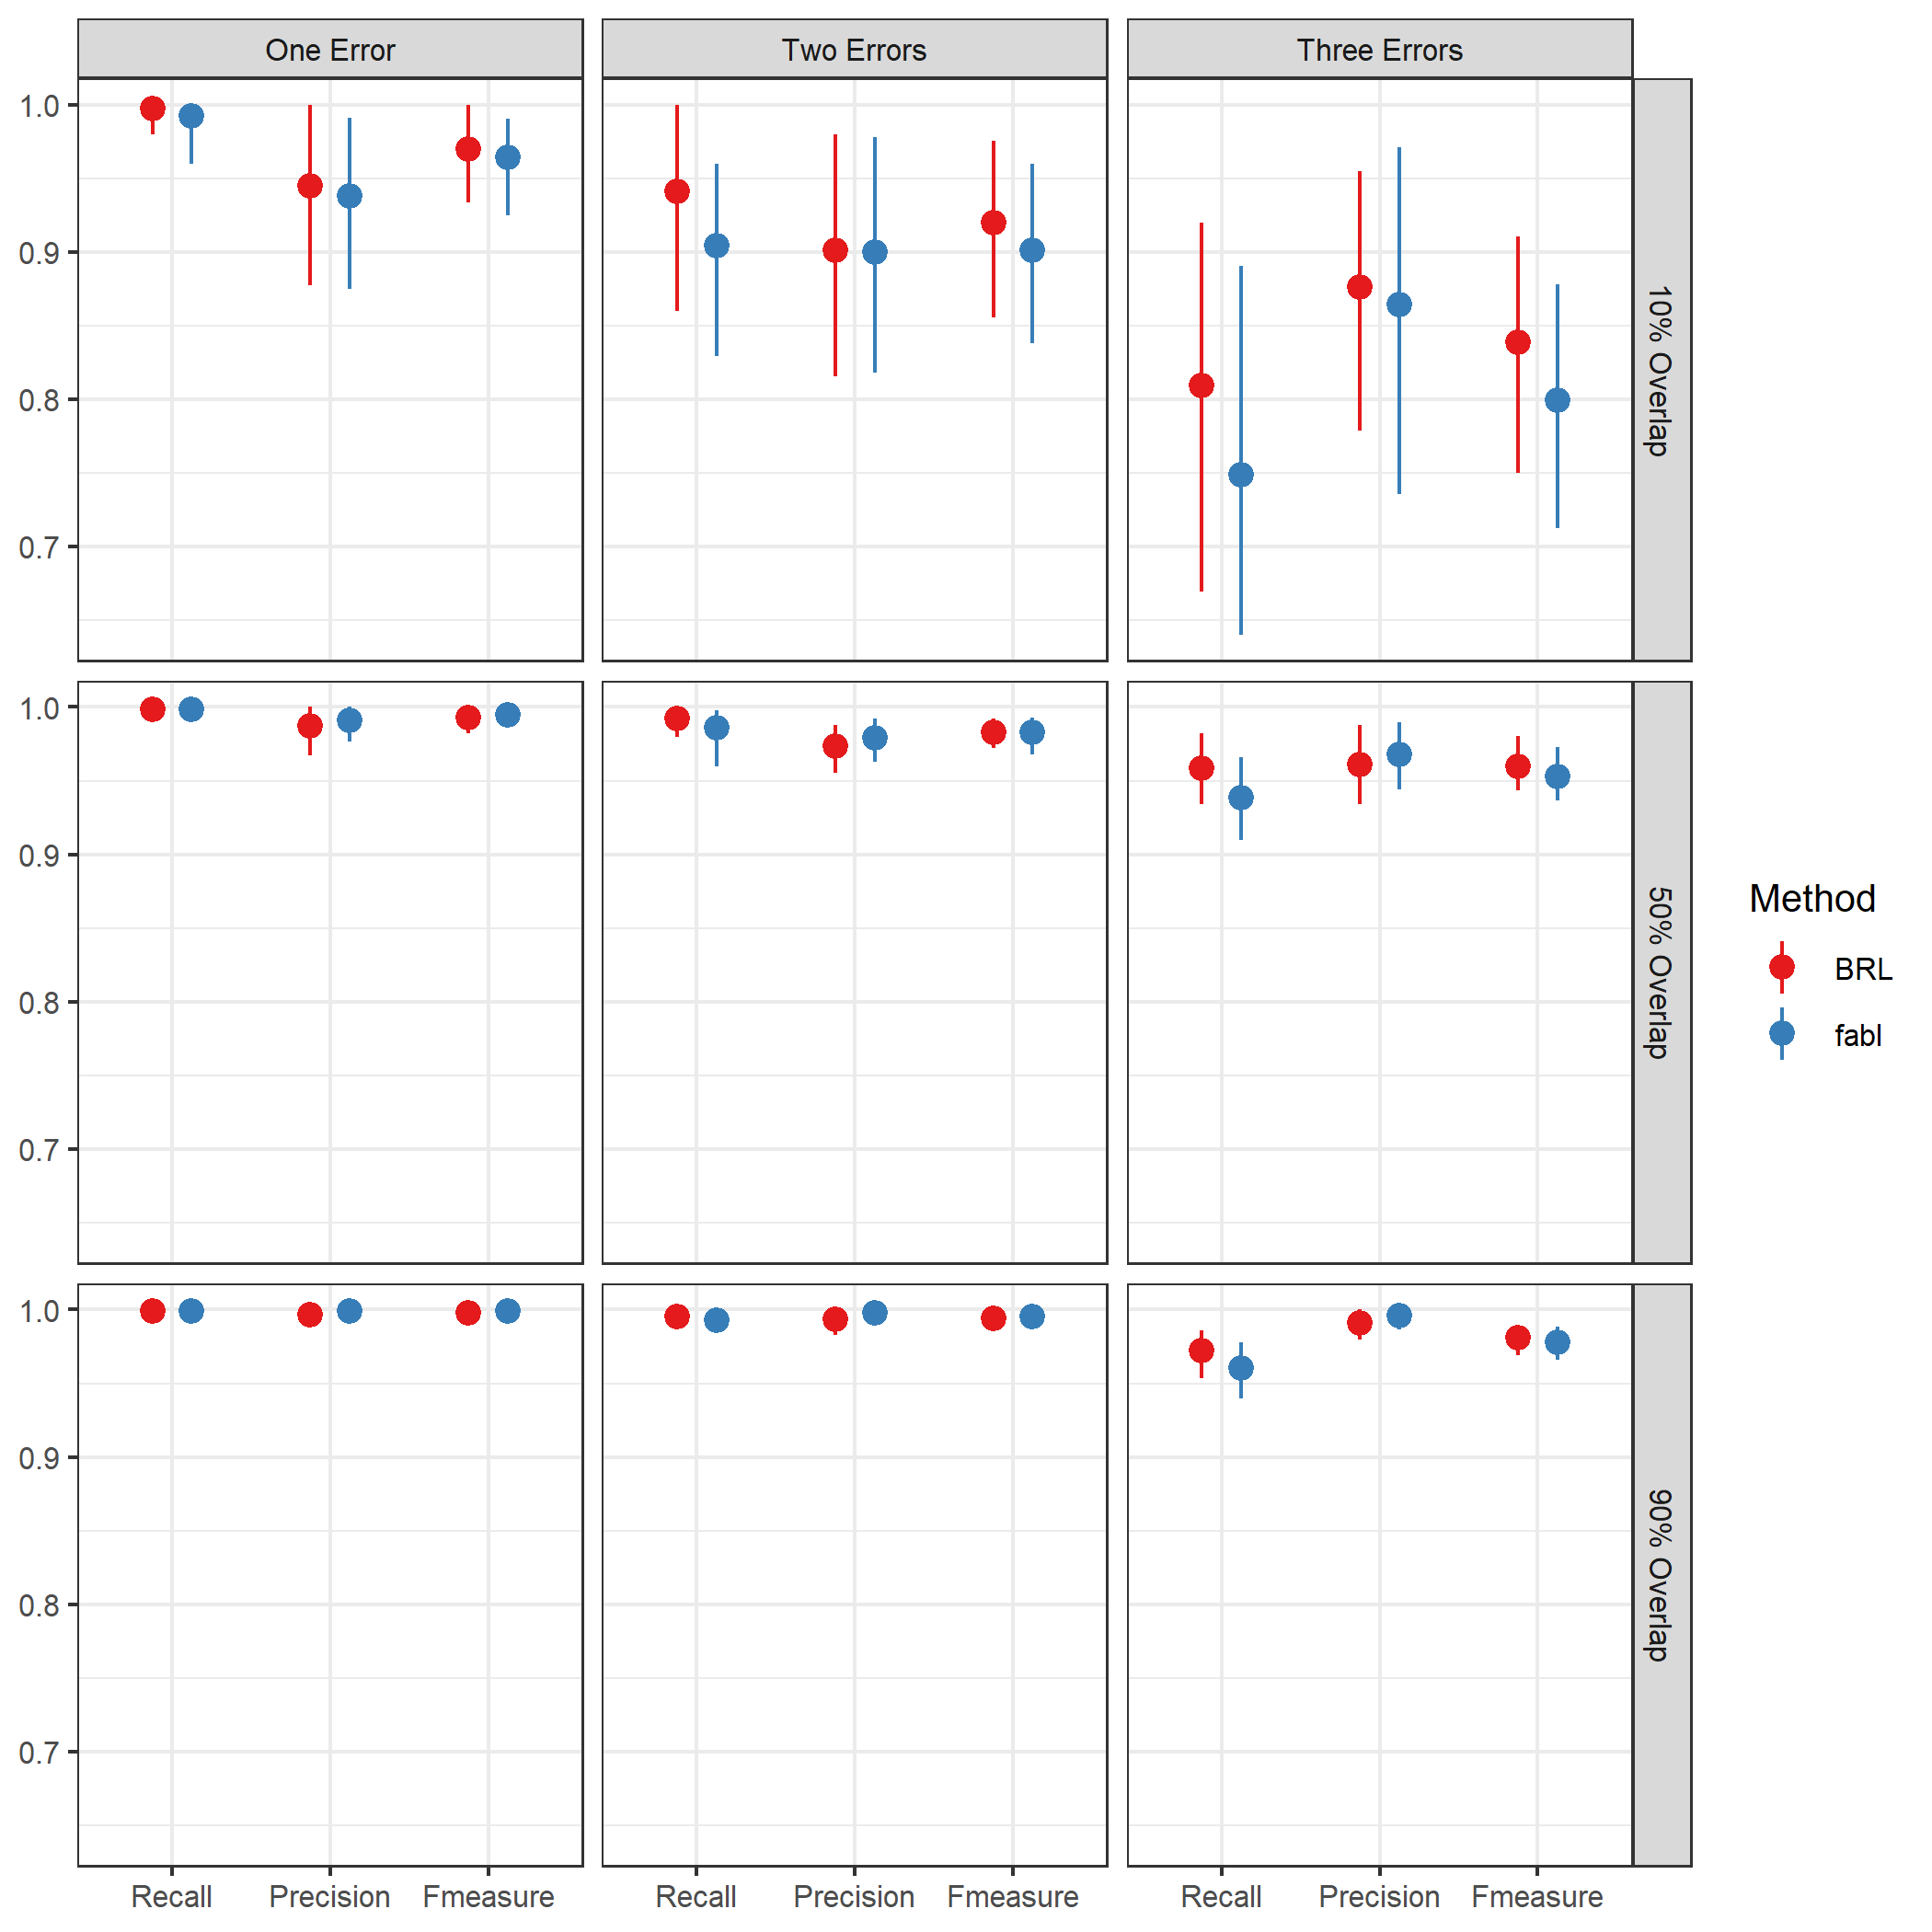
\includegraphics[width=0.6\textwidth]{../notes/figures/sadinle_sim_plot2} 
\caption{Posterior means and credible intervals for accuracy metrics under the replication of simulation study from \cite{sadinle_bayesian_2017}. For each level of overlap and each level of error, we have 100 paired sets of 500 records. We see comparable performance for all levels of error and overlap.}
\label{fig:sadinle_simulation}
	\end{center}
\end{figure}

\hypertarget{partial}{%
	\subsection{Accuracy under Partial Estimates}\label{partial}}

By leaving $\theta_{10} = \theta_{01} = 1$ and $\theta_{11} = 2$, but setting $\theta_R = 0.1$, we allow the model to decline to decide a match for certain records, with nonassignment being 10\% as costly as a false match. In this context, we are no longer focused on finding all true matches, but rather protecting against false matches. Thus, instead of recall, we use the \emph{negative predictive value} (NPV), defined as the proportion of non-links that are actual non-matches. Mathematically, $\text{NPV} = \sum_{j=1}^{n_2} I(\hat{Z}_j = Z_j = n_1 + j)$/$\sum_{j=1}^{n_2} I(\hat{Z}_j = n_1 + j)$. We continue to use the precision, which is renamed the \emph{positive predictive value} (PPV) in this context. Lastly, we also report the rejection rate (RR), or how often the model declines to make a linkage decision, defined as RR = $\sum_{j=1}^{n_2} I(\hat{Z}_j = R)$.

In Figure~\ref{fig:sadinle_simulation_partial}, we see that \texttt{fabl} maintains equivalently strong PPV as \texttt{BRL} across all linkage settings. However, with high amounts of overlap, the rejection rate under \texttt{fabl} rises, leading to a decrease in NPV. Since \texttt{fabl} does not remove previously matched records from consideration for a new record, posterior probability of matches can at times be more split across different records; in contrast, \texttt{BRL} is able to maintain higher confidence in matches in this setting. In practice, it is rare to encounter linkage tasks with 90\% overlap, so we remain confident in \texttt{fabl}'s performance. If one wishes to use partial estimates, \texttt{fabl} will possibly leave more linkages for the modeller to match by hand that would be left under \texttt{BRL}, but the decisions made by each method will have nearly equal accuracy. 

%This is reasonable because large numbers of errors blur the distinction between matched and nonmatched pairs, leading to situations where one record in $\bf{X}_2$ has multiple plausible matches in $\bf{X}_1$, so that posterior match probability is split across more records.

\begin{figure}[h!]
\begin{center}
	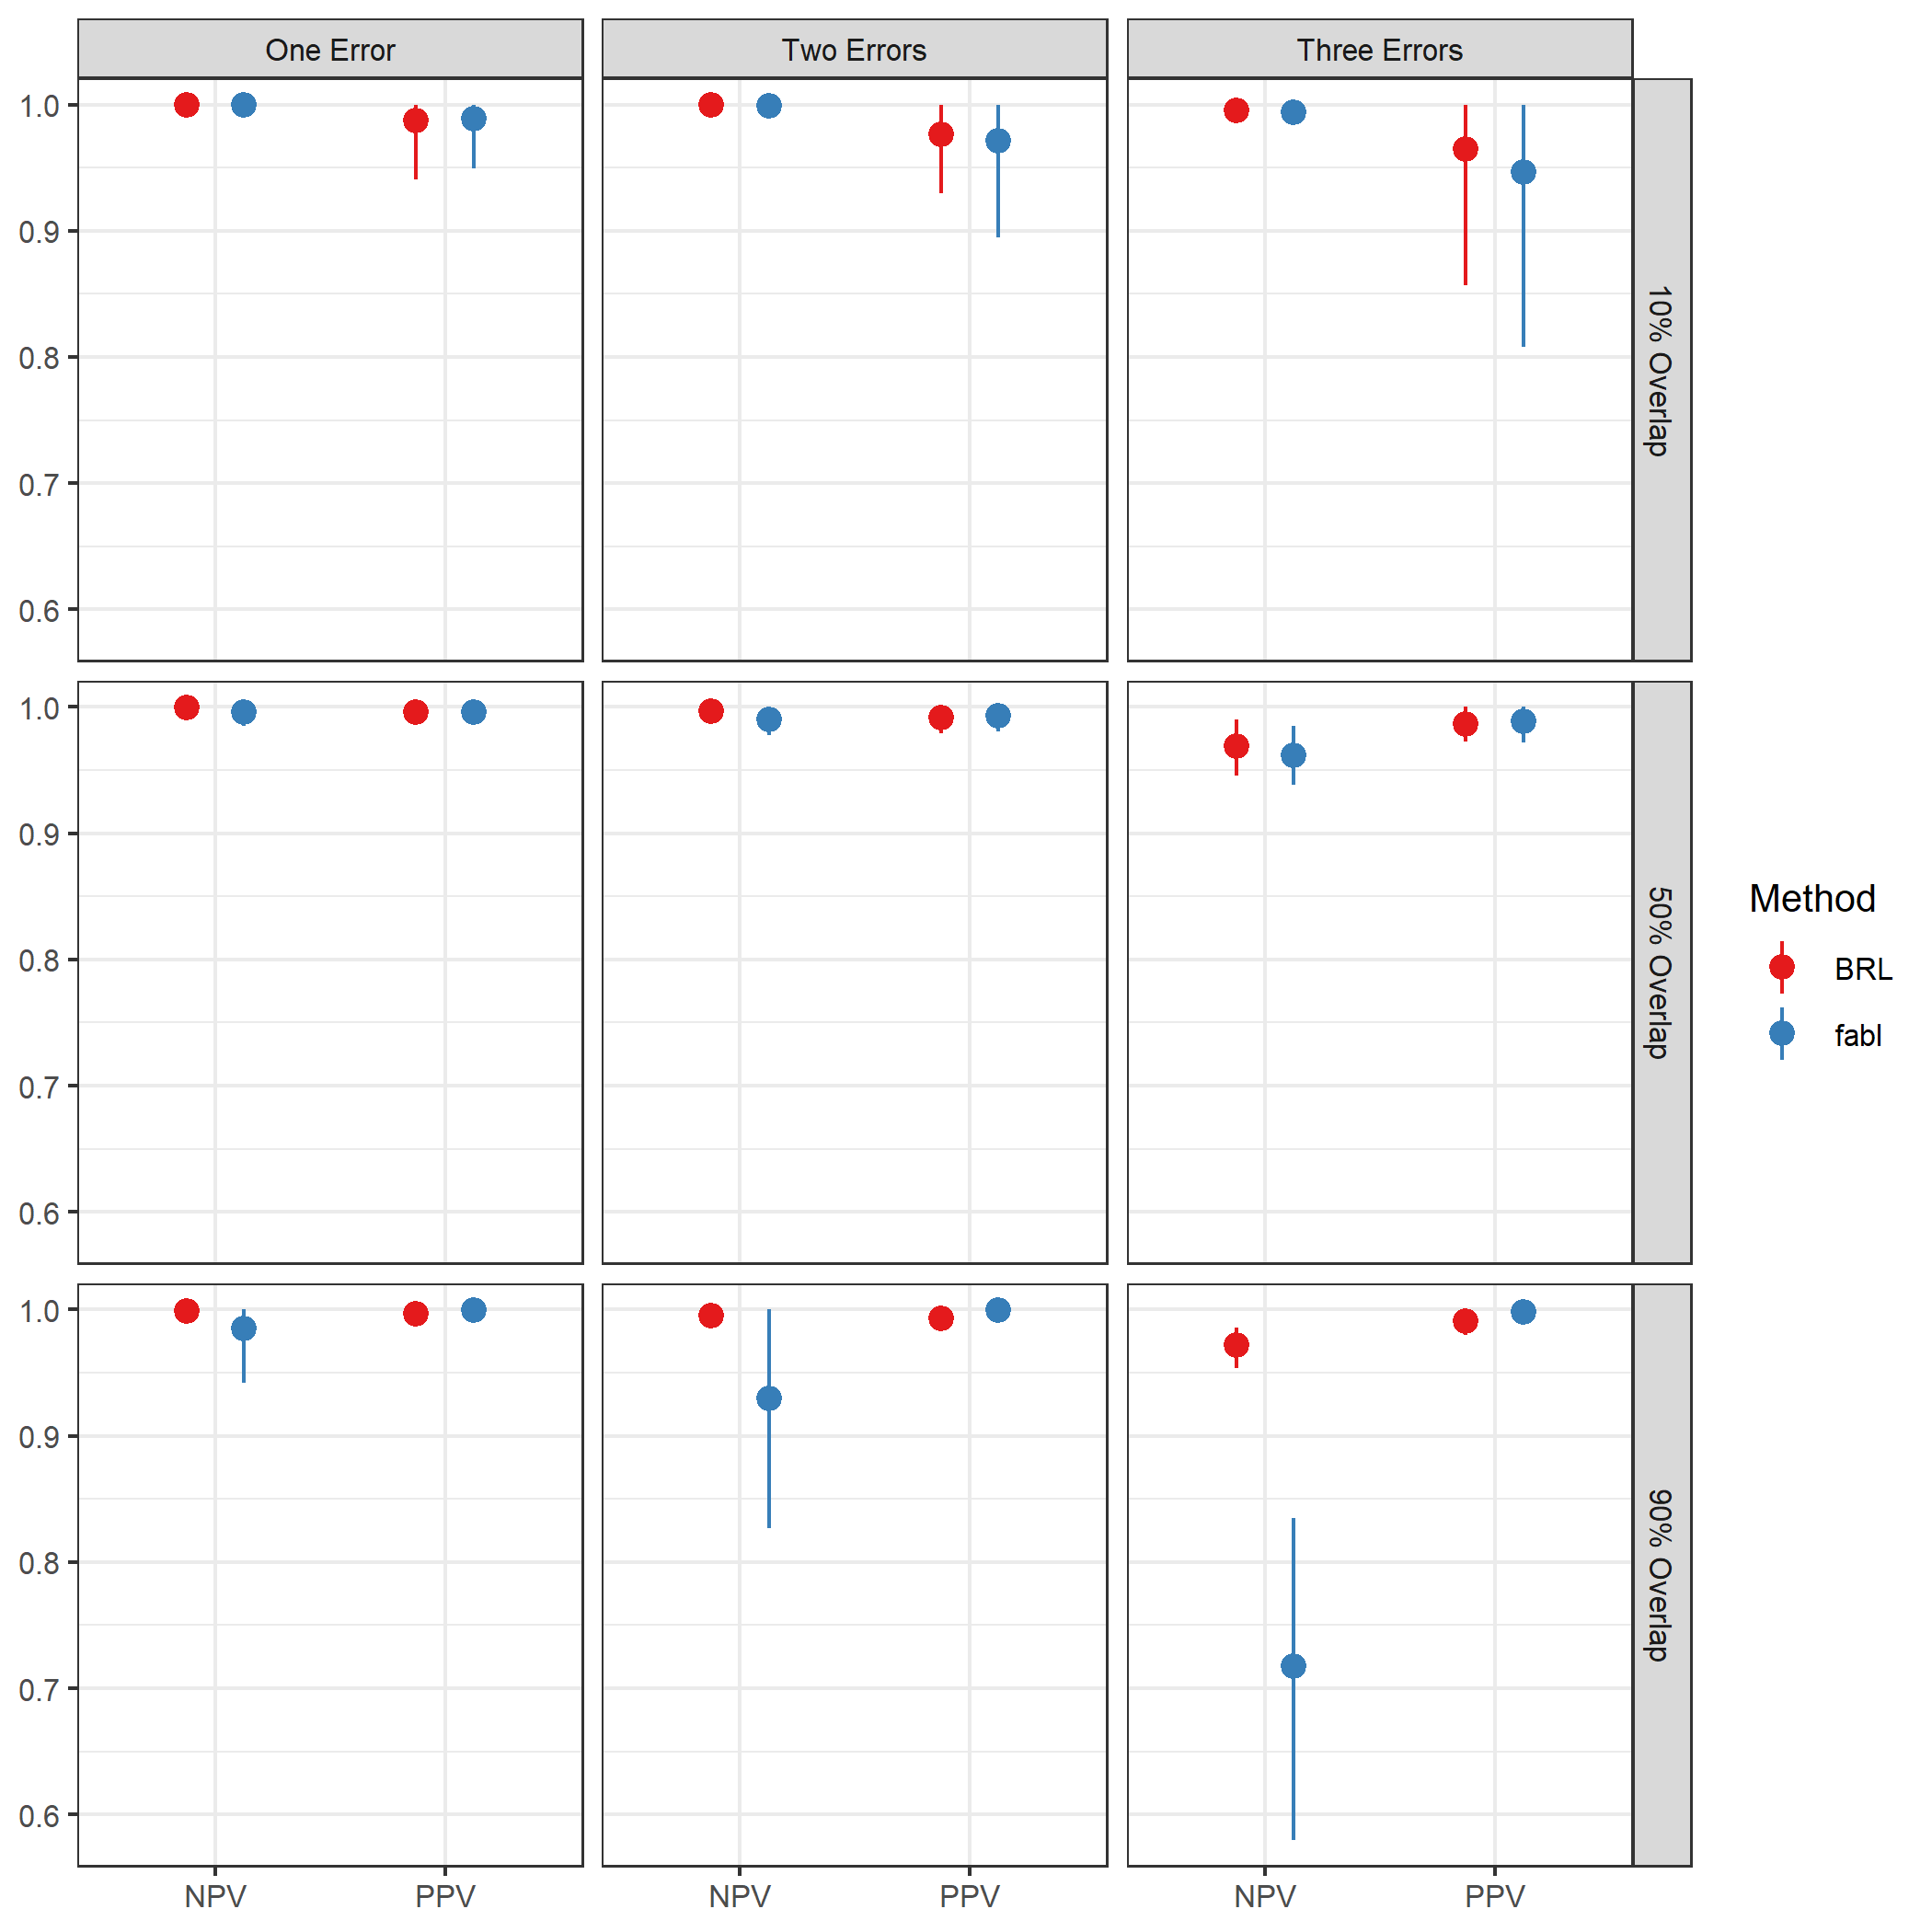
\includegraphics[width=0.6\textwidth]{../notes/figures/sadinle_sim_plot_partial} 
	\caption{Negative predictive value (NPV) and positive predictive value (PPV) on simulated datasets. We see poorer performance for \texttt{fabl} only in situations with high overlap.}
	\label{fig:sadinle_simulation_partial}
\end{center}
\end{figure}

\hypertarget{speed}{%
	\subsection{Speed}\label{speed}}

To demonstrate speed, we generate comparison vectors from pre-specified
distributions so that we can easily increase the size of the linkage
problem. The distributions used (see Table~\ref{Tab:distributions}) are meant to emulate the rates of agreement across first name, last name, day of birth, and month of birth.  For example, $u^{\text{month, agree}} = P(\text{Records have same birth-month} \mid \text{Nonmatch}) = \frac{1}{12}$. The parameters for year would vary largely by context, so we chose them here to adjust the desired difficulty of the linkage task.For simplicity, we consider only exact matching, so a vector (1, 0) corresponds to
agreement and (0, 1) to disagreement. We simulate these data for
different values of \(n_1\) and \(n_2\), and compare the run-time of
\texttt{fabl} against \texttt{BRL}. Since we have 5 binary comparison fields, the number is unique patterns \(P\) is bounded above by \(2^5 = 32\), a bound which is
consistently attained in the larger simulations.

\begin{table}[h!]
	\centering
	\begin{tabular}{rrr}
		\hline
		& m & u \\ 
		\hline
		fname & $\left(\frac{19}{20}, \frac{1}{20}\right)$ & $\left(\frac{1}{100}, \frac{99}{100}\right)$ \\ 
		lname & $\left(\frac{19}{20}, \frac{1}{20}\right)$ & $\left(\frac{1}{100}, \frac{99}{100}\right)$ \\ 
		day & $\left(\frac{19}{20}, \frac{1}{20}\right)$ & $\left(\frac{1}{30}, \frac{29}{30}\right)$ \\ 
		month & $\left(\frac{19}{20}, \frac{1}{20}\right)$ & $\left(\frac{1}{12}, \frac{11}{12}\right)$ \\ 
		year & $\left(\frac{19}{20}, \frac{1}{20}\right)$ & $\left(\frac{1}{12}, \frac{11}{12}\right)$ \\ 
		\hline
	\end{tabular}
	\caption{Distributions used for $m$ and $u$ probabilties in simulation studies}\label{Tab:distributions}
\end{table}

In Figure~\ref{fig:speed1}, we see that at low data size, \texttt{BRL} outperforms, but that
\texttt{fabl} is significantly faster at handling larger data. In
particular, run-time for \texttt{BRL} seems to grow quadratically (or
linearly with the size of both $\bm{X}_1$ and $\bm{X}_2$) while run-time for
\texttt{fabl} seems to grow linearly (in the size of $\bm{X}_2$).

\begin{figure}[h!]
	\begin{center} 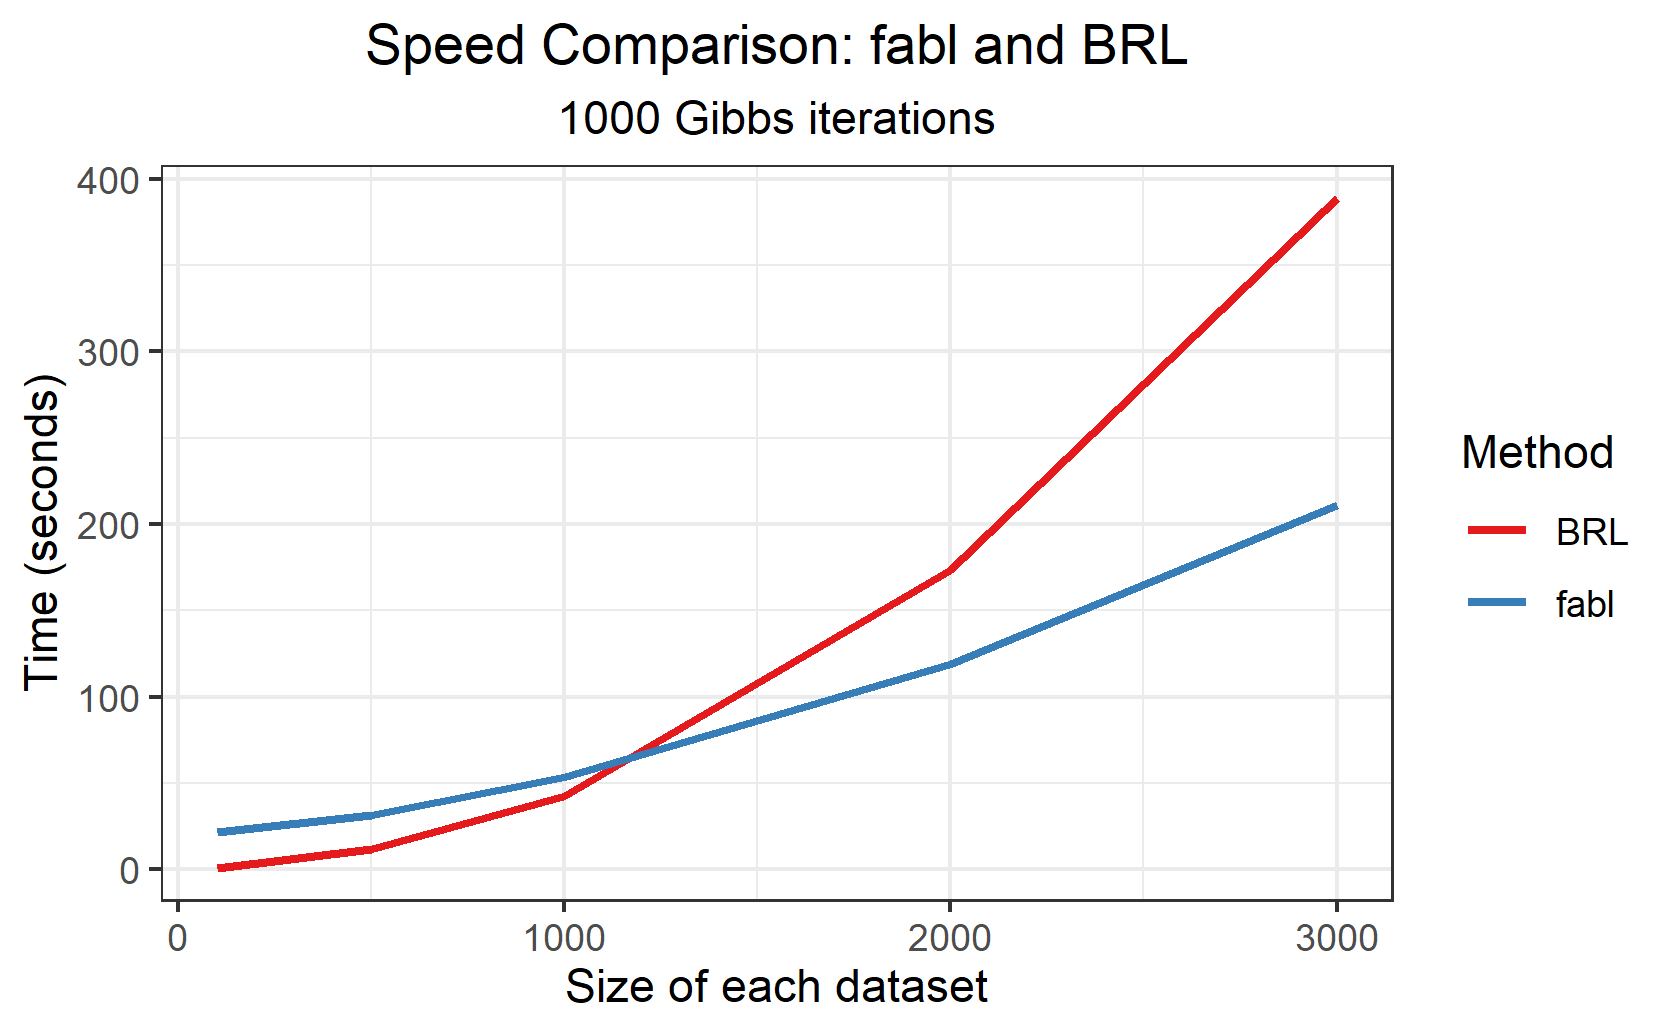
\includegraphics[width=0.6\textwidth]{../notes/figures/sadinle_speed_plot2} 
	\caption{Run-time for BRL and fabl to run 1000 Gibbs iterations, including hashing step for fabl, for increasing values of both $n_A$ and $n_B$. We see near quadratic growth in runtime for BRL, and near linear growth for fabl.}\label{fig:speed1}
	\end{center}
\end{figure}

The above discussion suggests that for fixed \(n_2\), computation time
should remain mostly constant with growing \(n_1\). Simulation study
suggests that this is true. In Figure~\ref{fig:speed2} fixing \(n_2 = 500\), we
see linear growth for the run-time under \texttt{BRL} as \(n_1\)
increases, with much more static run-time under \texttt{fabl}. The
slight increases in run-time that we do see are due primarily to the
hashing step, which again can be run in parallel for large data.

\begin{figure}[h!]
	\begin{center} 
\includegraphics[width=0.6\textwidth]{../notes/figures/speed_plot_fixed_nB} 
	\caption{Run-time for BRL and fabl to run 1000 Gibbs iterations, including hashing step for fabl, with increasing $n_A$, and $n_B$ fixed at 500. We see linear growth in runtime for BRL, and near constant runtime for fabl.}\label{fig:speed2}
	\end{center}
\end{figure}

We note here that \texttt{BRL} is coded in C, which makes for unfair
comparison against \texttt{fabl}, currently only built in R.
Additionally, although \texttt{fabl} is amenable to parallelization,
this simulation was run on a single core. Running \texttt{fabl} in C++
with paralellization for the hashing step and sampling the matching
status of the record pairs should lead to even more computational gains.

\hypertarget{scale}{%
	\subsection{Scaling to a Larger Simulation Study}\label{scale}}

To demonstrate the scale of the linkage tasks possible under \texttt{fabl}, we concatenate two sets of 40 simulated datasets from the original simulation studies of \cite{sadinle_bayesian_2017}, creating two larger files, each of 20,000 records (40,000 records total). Under standard Fellegi Sunter procedures, this would require 400,000,000 comparison vectors, each consisting for four integers, resulting in a final comparison matrix about 6.4 GB in size. Under default settings on a personal computer, \texttt{R} does not allow storing an object this size, so \texttt{BRL} is not usable on this linkage task. Through \texttt{fabl} however, using just one machine, we sequentially compare records across chunks, hash results, and then synthesize summary statistics for the entire simulation.  
 
For simplicity, we partition one dataset into 20 smaller chunks, and leave the second dataset fully intact. We compare records, hash results, and then synthesize summary statistics for all 20 chunk comparisons. The resulting data object is only 90 MB, about 1\% the size of the object required under the standard method. Executed sequentially, these comparisons and the Gibbs sampler take about one hour to run. However, this could be substantially sped up using distributed computing.

Turning to evaluation metrics, this simulation achieved 96.5\% recall and 97.7\% precision, with an overall F-measure of 97.1\% F-measure. The reader will note that this slightly worse performance than witnessed in the smaller simulation studies; this is expected because it is naturally more difficult to link more files with the same amount of information. With more linkage fields, \texttt{fabl} maintains the high accuracy in Section~\ref{accuracy}. 

\section{Application to Civilian Casualties from the El Salvadoran Civil War}
\label{sec:case-studies}

In this section, we revisit an application to the El Salvadoran Civil War, where we estimate the number of individuals recorded in both datasets. Though the data files used here are small, this study shows how the computational complexity of \texttt{fabl} depends on the number of unique agreement patterns found in the data, and how significant computational gains can be achieved by simplifying the construction of the comparison vectors. This case study also considers the ramifications of independently sampling $Z_j$ rather than strictly enforcing one-to-one matching as done by \texttt{BRL}. 

\subsection{El Salvadoran Civil War}
\label{el_salvador}

The country of El Salvador was immersed in civil war from 1980 to 1991,
and throughout the time, several organizations attempted to document
casualties of the conflict. When estimating the total number of
casualties, one cannot simply sum the numbers recorded by each
organization, as it is likely that the same individuals are recorded in
multiple casualty lists. This is an important step in estimating the total number of deaths from a conflict using multiple systems estimation \citep{lum2013applications}. We utilize lists of casualties from the war, one collected by El Rescate - Tutela
Regal (ERTL) and another from the Salvadoran Human Rights Commission (CDHES, by its
acronym in Spanish).\footnote{We thank the Human Rights Data Analysis Group (HRDAG) for granting access to this data.} The ERTL dataset consists of digitized denunciations that
had been published throughout the conflict, and the CDHES dataset consists
of casualties that had been reported directly to the organization \citep{howland2008rescate, ball2000salvadoran}. The ERTL required additional investigation before recording denunciations as human rights abuses, and reports to the CHDES were made shortly after the events occurred; thus, both datasets are thought to be fairly reliable.

There are several challenges with working with this data. Firstly, both
datasets have been automatically digitized, which inherently leads to
some degree of typographical error. Additionally, the only fields recorded are given name, last name, date of death, and place of death; it is relatively common for a
parent and child to share the same given name, resulting in
indistinguishable records for two different individuals. This last point
nearly breaks the earlier mentioned assumption that there are no
duplicates within files, and reveals a key difference between
\texttt{BRL} and our proposed method.

Following \cite{sadinle_bayesian_2017}, we utilize records that have non-missing entries for given and last name, which results in \(n_1 = 4420\) files in CHDES and \(n_2 = 1323\) files in ERTL. We standardized names to account for common misspellings and used a modified Levenstein distance when comparing names to account for the fact that second names are often omitted in Spanish. Place of death is recorded by municipality and department within that municipality; however, since department was missing in 95\% of records in CHDES and 80\% of records in ERTL, this was excluded from our analyses. Thus, we conduct record linkage using given name, last name, municipality, and day, month, and year of death. We again use flat priors for the \(\bm{m}\) and \(\bm{u}\) parameters.

To mirror the original implementation of \cite{sadinle_bayesian_2017}, we first construct the comparison vectors using four levels of agreement for each field, according to the thresholds provided in Table~\ref{Tab:el_salvador_cutoffs_1}. Gibbs sampling for these comparison vectors took 422 seconds for our proposed method, \texttt{fabl}, and 240 for \texttt{BRL}. However, we observed that posterior distributions of several levels of the \(\bm{m}\) and \(\bm{u}\) parameters were nearly identical, and that of the \(4^5 \times 2 = 2048\) possible agreement patterns, only 1173 were realized in the data. This leads us to believe that such high number of agreement levels creates unnecessary distinctions in the data and makes the comparison vectors less interpretable. 

\begin{table}
	\begin{tabular}[h!]{ll|llll}
		\hline
		\multicolumn{2}{c|}{ } & \multicolumn{4}{c}{Level of Disagreement} \\
		\cline{3-6}
		Fields & Similarity & 1 & 2 & 3 & 4\\
		\hline
		First and Last Name & Modified Levenstein & 0 & (0, .25] & (.25, .5] & (.5, 1]\\
		Year of Death & Absolute Difference & 0 & 1 & 2 & 3+\\
		Month of Death & Absolute Difference & 0 & 1 & 2-3 & 4+\\
		Day of Death & Absolute Difference & 0 & 1-2 & 3-7 & 8+\\
		Municipality & Binary & Agree & Disagree &  & \\
		\hline
	\end{tabular}
	\caption{Construction of comparison vectors for El Salvador data resembling original implementation from \citep{sadinle2018bayesian}. This set up leads to 2048 possible agreement patterns in total.}\label{Tab:el_salvador_cutoffs_1}
\end{table}

Therefore we re-ran our analysis with fewer agreement levels for each field according to Table~\ref{Tab:el_salvador_cutoffs_2}, and obtained analogous inference. With 216 possible agreement patterns, 159 were realized in the data, and our proposed method, \texttt{fabl} became much faster, finishing in 61 seconds. Meanwhile \texttt{BRL} took 239 seconds, relatively unchanged from the first implementation. This demonstrates the way that the computational complexity of our method depends on the number of unique agreement patterns, and how significant computational gains can be made by simplifying the construction of the comparison vectors. The estimates of the \(\bm{m}\) parameters under each method are very similar, as shown in Figure~\ref{fig:m-and-u}. Additionally, traceplots for parameters of interest are provided in Appendix \ref{app:appendix-es}

\begin{table}
	\centering
	\begin{tabular}[h!]{ll|lll}
		\hline
		\multicolumn{2}{c|}{ } & \multicolumn{3}{c}{Level of Disagreement} \\
		\cline{3-5}
		Fields & Similarity & 1 & 2 & 3\\
		\hline
		First and Last Name & Modified Levenstein & 0 & (0, .25] & (.25, 1]\\
		Year of Death & Binary & Agree & Disagree & \\
		Month of Death & Binary & Agree & Disagree & \\
		Day of Death & Absolute Difference & 0 & 1 & 2+\\
		Municipality & Binary & Agree & Disagree & \\
		\hline
	\end{tabular}
	\caption{Construction of comparison vectors for El Salvador for increased speed under \texttt{fabl}. This set up leads to 216 possible agreement patterns in total.}\label{Tab:el_salvador_cutoffs_2}
\end{table}

Through \texttt{fabl}, we arrive at a Bayes estimate of 179 individuals recorded in both datasets. We calcuate posterior samples of the size of the overlap across files by finding the number of matches found in each iteration of the Gibbs sampler, and subtracting the number of matches that violate one-to-one matching. The posterior 95\% credible interval for the overlap across files is (206, 238), indicating that the Bayes estimate is quite conservative. This is because there a large number of records in ERTL for which there are multiple plausible matches in CDHES; \texttt{fabl} recognizes that a match exists among the several options, but is unable to definitely declare a specific pair as a match in the Bayes estimate. We also compute a partial estimate of the linkage structure, using $\theta_{10} = \theta_{01} = 1$, $\theta_{11} = 2$, and $\theta_R = 0.1$ as in the simulation study. Here, the Bayes estimate provides 136 matches of which the model is quite confident, and 175 records to verify manually; this means that after clerical review, the number of individuals replicated across datasets would fall in the interval (136, 311), encapsulating the posterior credible interval. More or fewer records could be indentified for clerical review by decreasing or increasing $\theta_R$. 

We see similar results under \texttt{BRL}, with a Bayes estimate of 181 individuals recorded in both datasets, a posterior 95\% credible interval of (211, 244), and a range of (140, 294) after the partial estimate and clerical review. 

\begin{figure}[h!]
	\begin{center}
		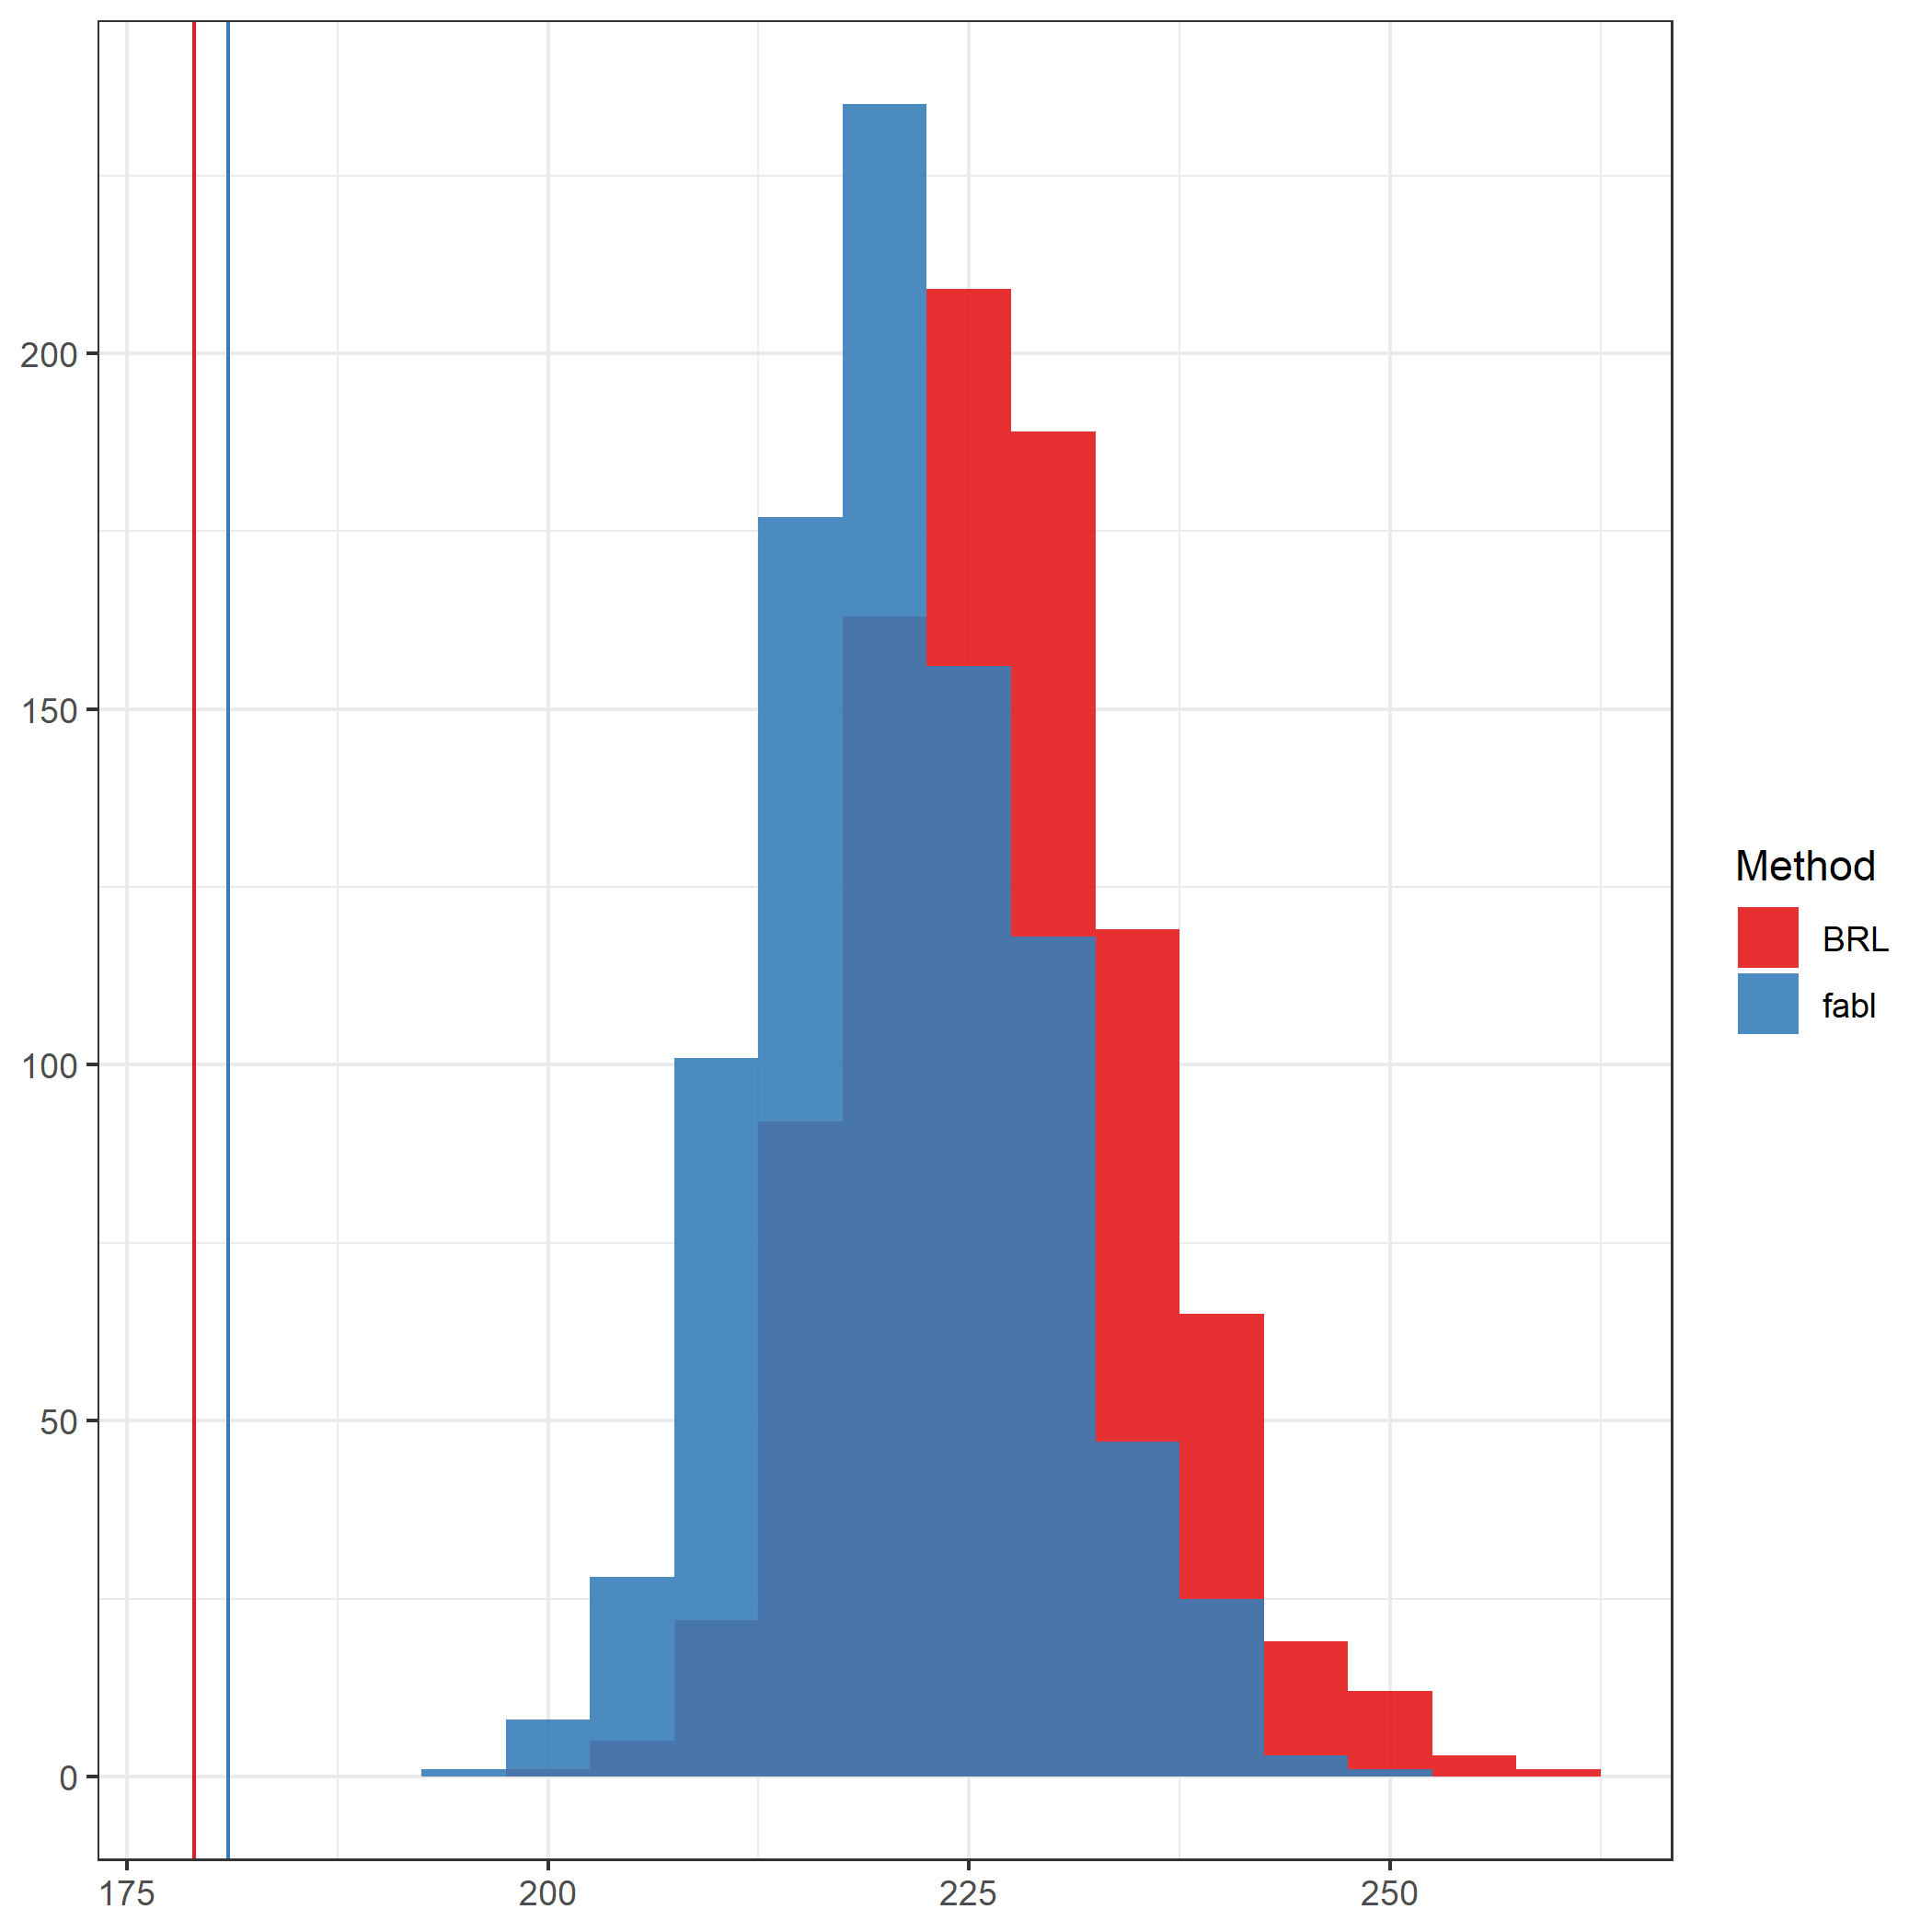
\includegraphics[width=0.6\textwidth]{../notes/figures/el_salvador/overlap_distribution_smallP_bayes}
		\caption{Posterior distribution and Bayes estimate of overlap across the two files. We note they are quite similar under both methods.}
		\label{fig:overlap-plot}
	\end{center}
\end{figure}


\begin{figure}[h!]
\begin{center}
	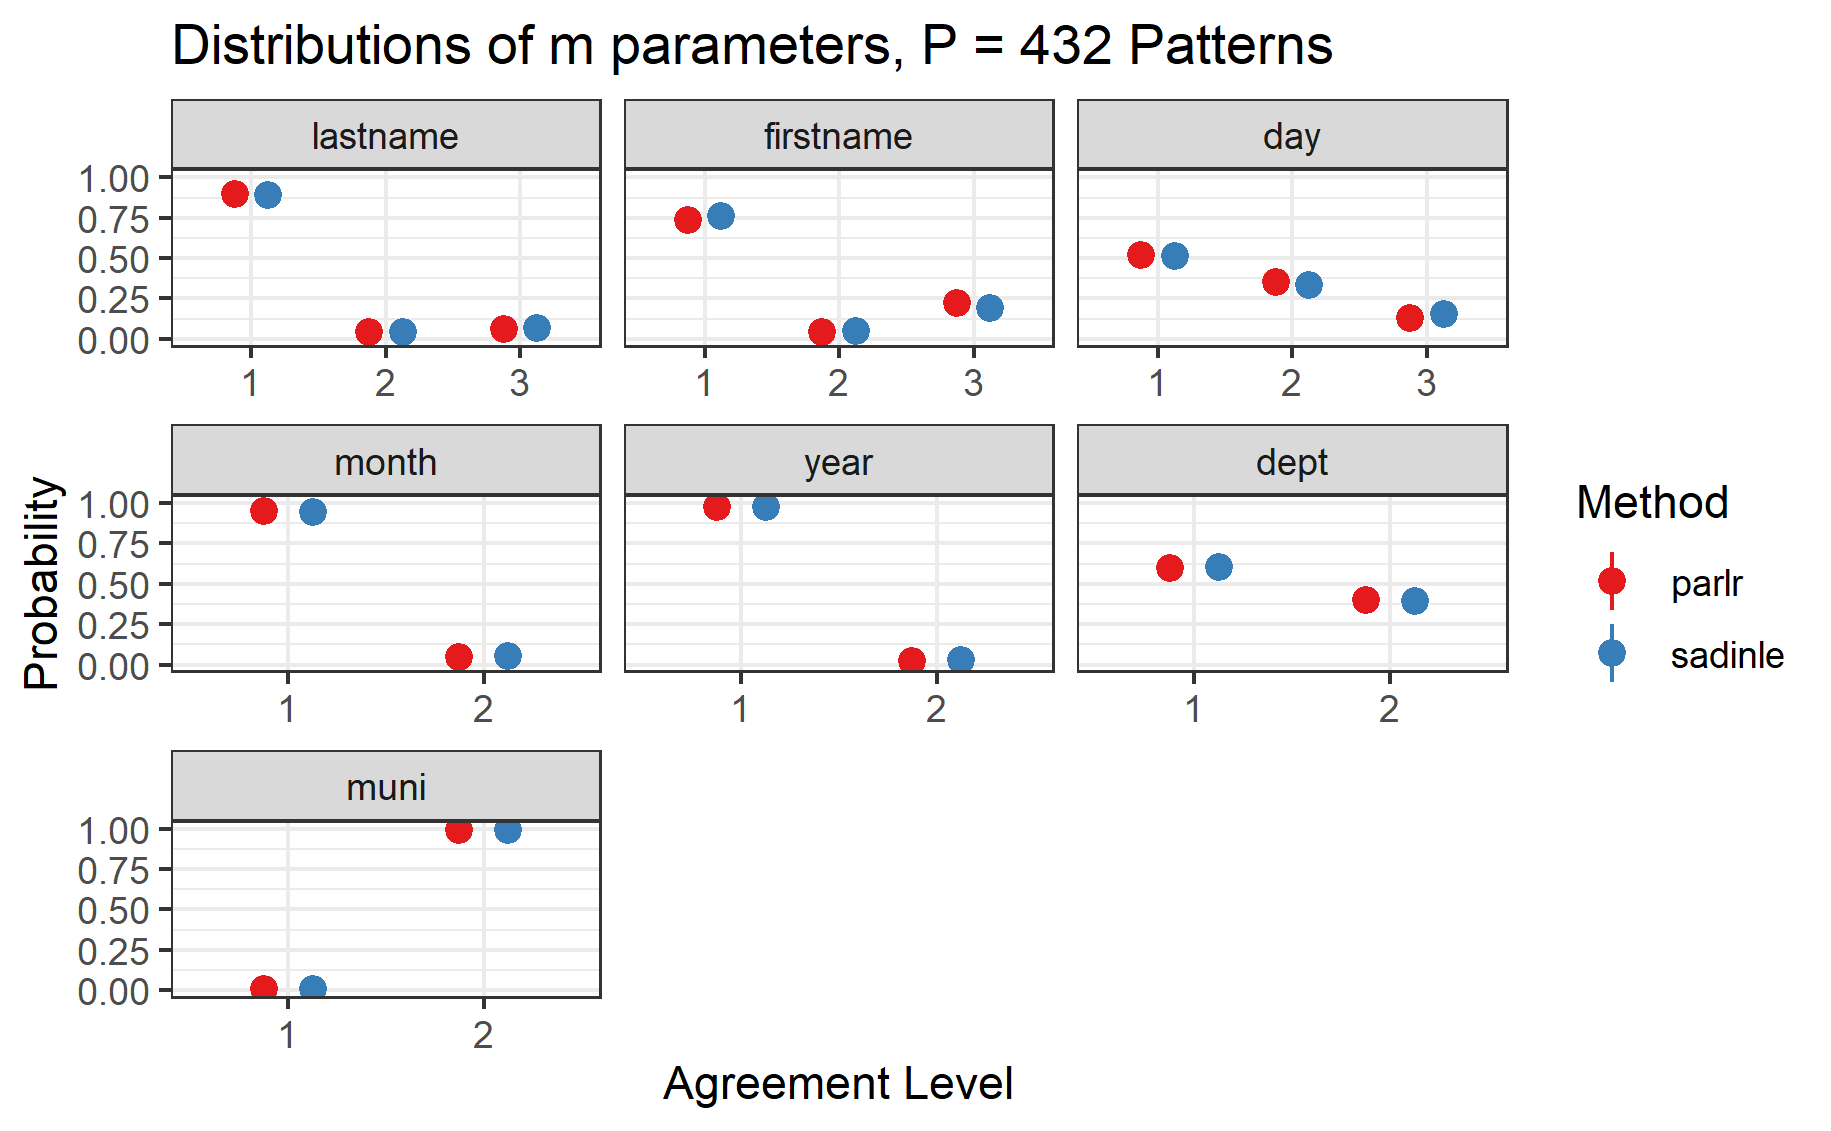
\includegraphics[width=0.6\textwidth]{../notes/figures/el_salvador/m_posterior_smallP} 
\caption{Posterior estimates of m parameters with 95\% credible intervals. We note they are quite similar across the two methods.}\label{fig:m-and-u}
\label{fig:m-and-u}
\end{center}
\end{figure}

\hypertarget{violations}{%
	\subsection{Violations of One-to-One Matching}\label{violations}}

As noted previously, the application exhibits many situations in which bipartite matching is difficult. To explore further, we calculate the number of matchings throughout the \texttt{fabl} Gibbs sampler that violate our one-to-one assumption, and find on average 26.17 matchings in violation. These matchings are impossible under the \texttt{BRL} Gibbs sampler, so examining these more closely can provide insight how each model handles situations in which one file in $\bm{X}_1$ has
multiple plausible matches in $\bm{X}_2$. 

%Figure~\ref{fig:overlap-plot} shows the posterior distribution for \(D\), the number of
%duplicates found in both databases for both \texttt{fabl} and \texttt{BRL}. We
%see that \texttt{fabl} consistently overmatches within each Gibbs
%iteration when compared to \texttt{BRL}, which is to be expected because
%\texttt{BRL} explicitly prevents matches that violate one-to-one
%matching throughout the entire sampler. Most of such matchings are due
%to the randomness in the sampling procedure, and they occur sporadically
%throughout the sampler in such a way that does not measurably influence
%the eventual Bayes estimate.

Table~\ref{Tab:rosa-maria} illustrates an example. Note that these records present a near violation of our assumption that there are no duplications within files; we continue to assume that records 825 and 826 in ERTL correspond to different individuals (most likely a mother and daughter), but their records are nearly identical. In addition, using the modified Levenstein distance, the comparison vectors \(\gamma_{2776, 825}\) and \(\gamma_{2776, 826}\) are exactly identical.

\begin{table}
	\centering
	\begin{tabular}[h!]{llllllll}
		\hline
		Record No. & Dataset & Last Name & First Name & Day & Month & Year & Dept \\
		\hline
		825 & CDHES & Pineda & Rosa & 6 & 4 & 1984 & NA\\
		826 & CDHES & Pineda & Rosa Maria & 6 & 4 & 1984 & NA\\
		2776 & ERTL & Pineda & Rosa Maria & 4 & 4 & 1984 & Cuscatlan\\
		\hline
	\end{tabular}
	\caption{Example of linkage situation in which record 2776 in ERTL has multiple plausible matches in CDHES, leading to undesirable behavior both \texttt{fabl} and \texttt{BRL}.}\label{Tab:rosa-maria}
\end{table}

Figure~\ref{fig:mixing-plot} shows the values that $Z_{825}$ and $Z_{826}$ take on throughout the Gibbs sampler, and demonstrates how each method handles this situation. Under \texttt{fabl}, both records in $\bm{X}_2$ match to the same record in $\bm{X}_1$ throughout the Gibbs process, creating consistent violations of one-to-one matching. Under \texttt{BRL}, the Gibbs process creates one matching configuration and stays there for a while. However, if one pair ``unmatches,'' then the other record has a chance to latch on. Then, the Gibbs process is stuck with that matching status for a while, resulting in a Gibbs process with poor mixing. 

Through its independent sampling,\texttt{fabl} allows the modeler to inspect records with multiple plausible matches, and if they desire, to then choose the record pairing with the highest posterior probability. \texttt{BRL} in contrast, in strictly enforcing one-to-one matching throughout the sampler, can lead to situations where none of the plausible matches reach the threshold to be identified through the Bayes estimate. Thus relaxing the one-to-one constraint has served as a useful tool for identifying model misspecification. 

\begin{figure}[h!]
\begin{center}
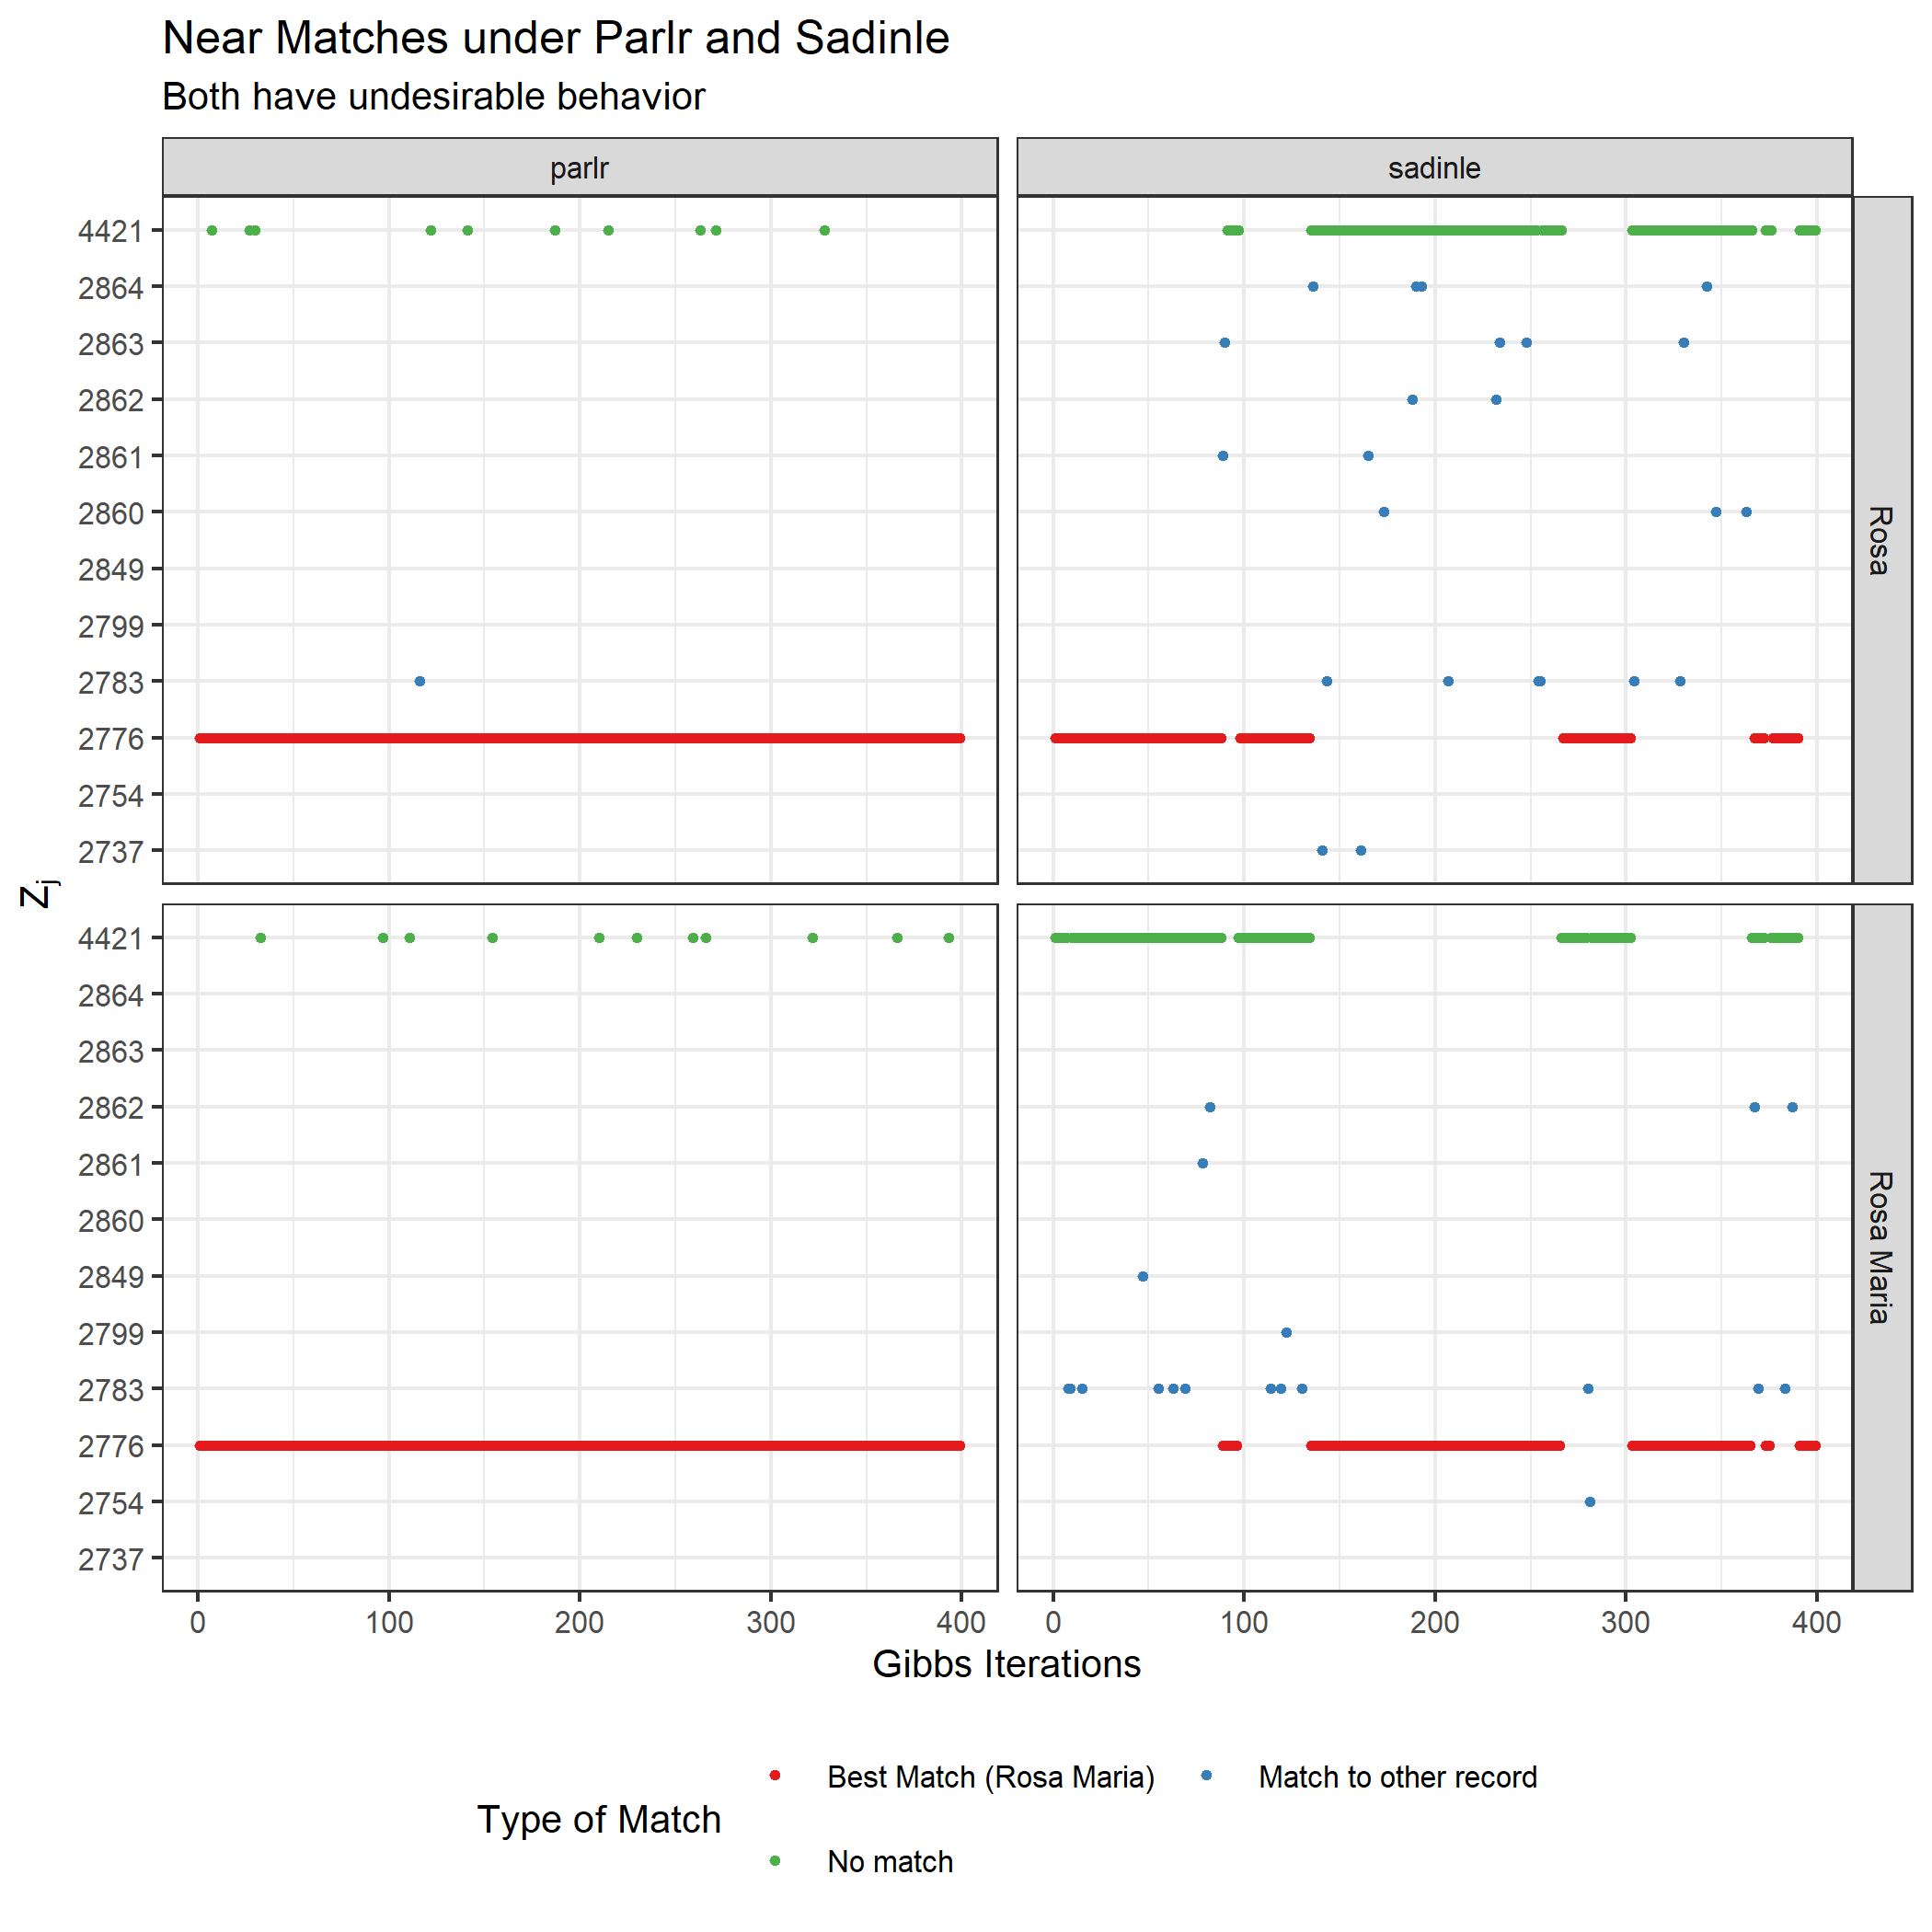
\includegraphics[width=0.6\textwidth]{../notes/figures/el_salvador/bad_mixing} 
\caption{Gibbs sampling in situation with multiple plausible matches. Under \texttt{BRL}, two records in ERTL compete for their most similar record, splitting the posterior probability. Under \texttt{fabl}, both record consistently match with their most similar record, consistently violating one-to-one matching.} \label{fig:mixing-plot}
\end{center}
\end{figure}

\section{Discussion}
\label{discussion}

\textcolor{red}{In this paper, we have proposed \texttt{fabl}, a Bayesian record linkage method that scales to large data sets. Specifically, our proposed hashing method}
%We have presented a method for Bayesian record linkage that is feasible for large datasets. In particular, our hashing procedure 
and model assumptions allow for a linkage procedure whose computational complexity does not scale with the size of the larger dataset, making our approach particularly powerful in linking records when one datafile is substantially smaller than the other.
\textcolor{red}{In our paper, we have provided details regarding derivations of conditional distributions and our proposed Gibbs sampler. In addition, we prove the computational complexity of our algorithm. In addition, we provided both simulation studies and revisited the same case study of the main methodology that we build upon.}  In our case study, we included an exploration of how to conduct record linkage when modeling assumptions are not met in practice. We explored ``one-to-many'' scenarios in which one record in $\bm{X}_2$ has multiple plausible matches in $\bm{X}_1$, and showed how both \texttt{fabl} and \texttt{BRL} demonstrated undesirable qualities. Other issues arise under ``many-to-one'' scenarios, where one record in $\bm{X}_2$ has multiple plausible matches in $\bm{X}_1$, and ``many-to-many'' scenarios in which there is duplication both across and within datasets. Extending \texttt{fabl} in such scenarios is currently investigation by the authors regarding future work. 

\textcolor{red}{Brian: could you talk about a few other directions that might be useful to take your work as this will come up in your prelim. For example, how might you extend beyond bipartite and still scale? Or what ideas do you think are the most exciting to take your work in next. This is your opportunity to talk about anything here and give a comment to the community about what you think is most important!} 

%Tuning \texttt{fabl} for use in these scenarios is one potential avenue for
%future work.

%\begin{figure}[t]
%	
%	{\centering 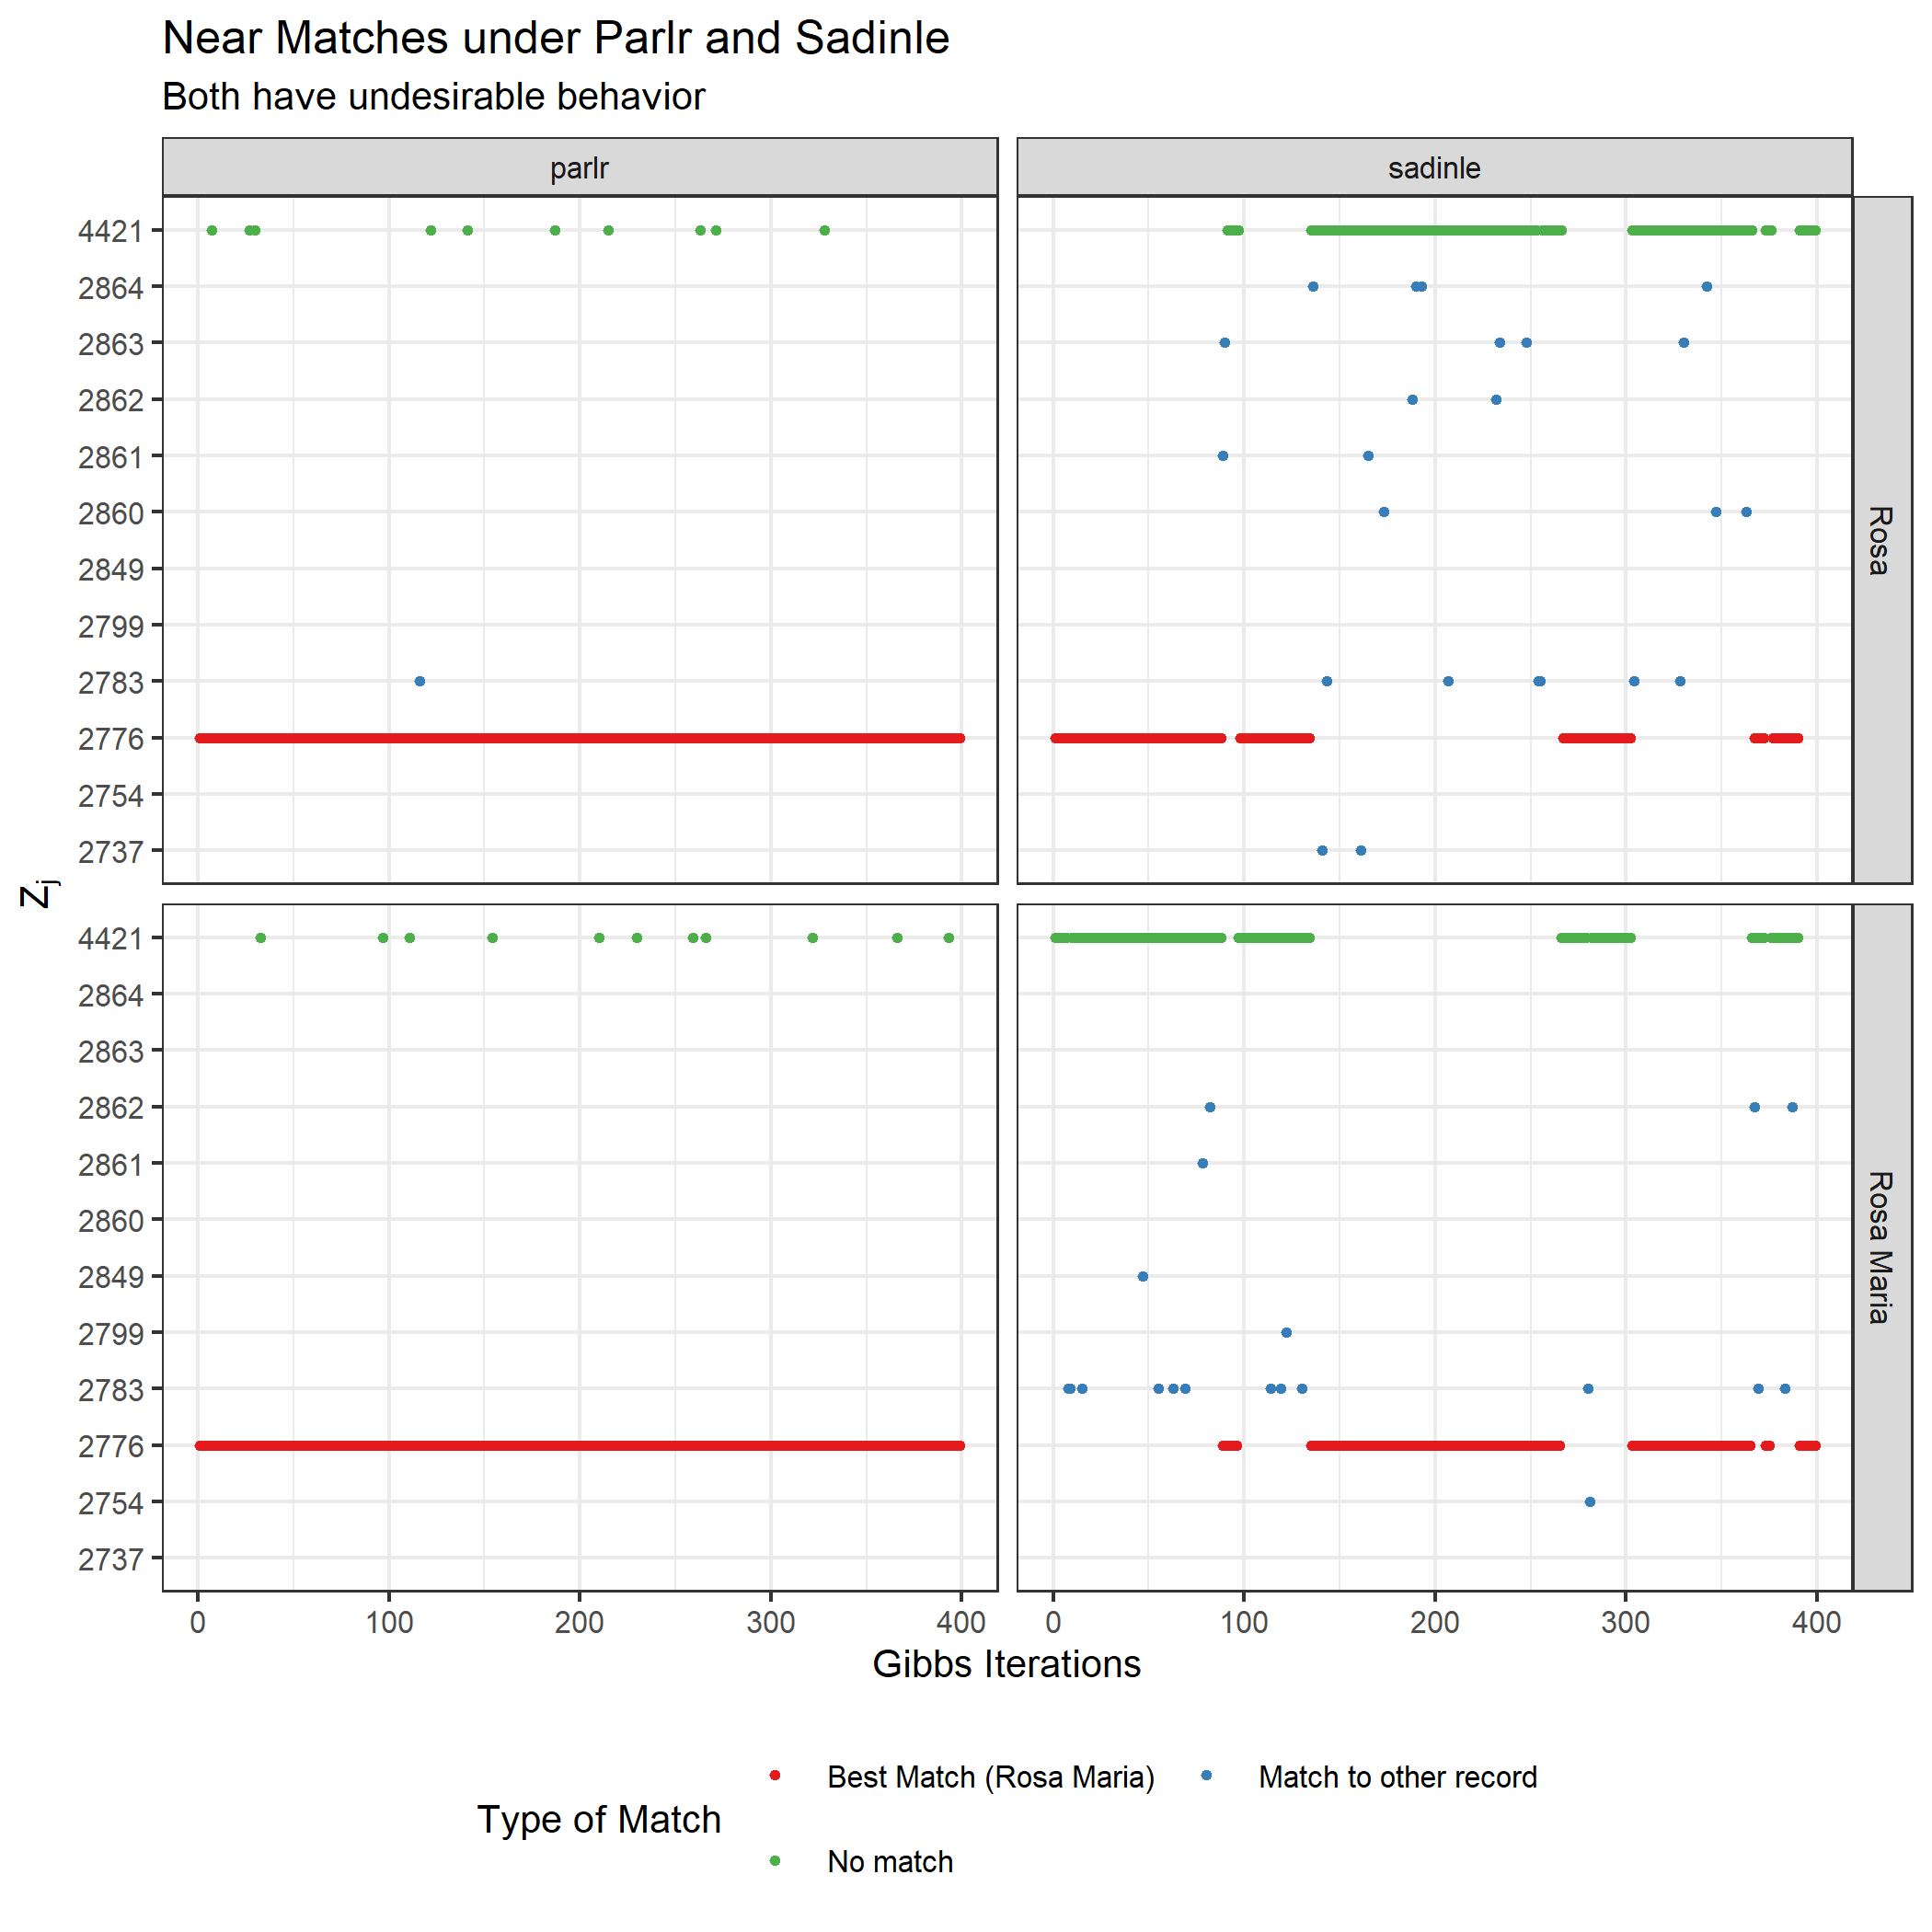
\includegraphics[width=0.6\textwidth]{../notes/figures/el_salvador/bad_mixing} 
%		
%	}
%	
%	\caption{Gibbs sampling in situation with multiple plausible matches.}\label{fig:mixing-plot}
%\end{figure}

%\subsection{National Long Term Care Survey}
%\label{nltcs} 
%
%The National Long Term Care Survey is a longitudinal study to track changes in health among Medicare recipients. It was conducted approximately every five years, and we concern ourselves here with linking records from years 1982 and 1989. The data only contains day, month, and year of birth, sex, state the individual lives in, and regional office. State and regional office have been anonymized, presented as numbers instead of their actual values. We construct the comparison vectors using only binary exact matching for each field, since there is no straightfoward way to incorporate partial matching in this context. The 1982 file contains $n_A = 20485$ records, 1989 file contains $n_B = 17466$ files, and the six linkage fields induces $2^6 = 64$ possible unique agreement patterns. We note that linkage quality is bound to be quite weak for many potential matches with such a large number of records and such limited identifying information.  
%
%With such large files, performing all-to-all comparisons under the original Fellegi-Sunter framework is infeasible. Indeed, this would require nearly 400 million comparison vectors, each containing 6 integer comparisons; the resulting data object would contain over 2 billion integers, and would require approximately 16 GBs of memory to hold. Instead, we take the partitioning approach reviewed in \ref{data-representation-hashing-and-storage}, and split each dataset into 10 smaller datasets. We use parallel computing on cluster service create the comparison vectors for each pair of data chunks, hash the results, and compress in size through storage efficient indexing. We then aggregate the results, creating a data object of just 87 MB, and proceed with the Gibbs Sampler. 
%
%Were a personal computer able to hold the 16 GB data object required by the direct approach, the Gibbs sampler under \texttt{BRL} would be tortuously slow, with computational complexity $O(n_A \times n_B \times F)$ where $n_A = 20485$. However, under \texttt{fabl} the sampler has complexity $O(P \times n_B \times F)$ where $P = 64$, so 1000 iterations of the Gibbs sampler are completed in just XX seconds. Posterior analysis yields an initial estimate of 9991 individuals linked across the the two datasets, and 8895 individuals linked once conflicts are resolved to ensure one-to-one matching. 
%
%Lastly, we comment on the significance of conducting this linkage without the use of deterministic blocking. With previous methods, one could link these two records by blocking on a certain field, and running separate Gibbs samplers on each of the separate blocks. This strategy drastically improves computation since it significantly reduces the number of comparison vectors that need to be formed and uses smaller data objects throughout the sampler. However, this computational savings comes at the cost of missing potential links, specifically in cases where the blocking variable is recorded in error. In this case, 62 of the matched pairs exhibit a disagreement in sex, 17 exhibit a disagreement in state, and 39 exhibit a disagreement in regional office. We have no way to verify that the matches found under \texttt{fabl} are indeed correct, so it is possible that matches found with such disagreements are false positives. Even if not, the modeler may conclude that, for example, 17 missed matches are a small price to pay to be able to block on state and run 50 smaller, independent linkage procedures. However, \texttt{fabl} allows the modeler to make this choice for themselves, rather than being forced to do so for computational reasons. Additionally, by running on the Gibbs sampler the entirety of both files, we achieve $m$ and $u$ parameters that are interpretale for the entire study, rather than separate parameters for each block. Although these $m$ and $u$'s are often regarded as nuisance parameters in the record linkage literature, \texttt{fabl} allows for study of these parameters that has been been possible before. 

\clearpage

\bigskip

\bibliographystyle{jasa}
\bibliography{biblio}

\clearpage

\section*{Appendix}
\label{sec:appendix}



\hypertarget{app:fabl-psuedocode}{%
	\subsection{Summary of Fast Beta Linkage Method}\label{app:fabl-psuedocode}}

\begin{algorithm}[h!]
	\begin{algorithmic}[1]
		
		\Procedure{Hashing and Preprocessing}{}
		\State Construct and enumerate set of unique patterns $\mathcal{P}$ from $F$ and $\{L_f\}$
		\State Partition files $\bm{X_1}$ and $\bm{X_1}$ into chunks $\{\bm{X_{1n}}\}$, $\{\bm{X_{2m}}\}$
		\For{each $n$, $m$}
		\State Create comparison vectors between $\bm{X_{1n}}$ and $\bm{X_{2m}}$
		\State Hash records to $\mathcal{R}_{nm}$ and calculate summary statistics $\mathcal{H}_{nm}$
		\State Use SEI to reduce memory usage; $\mathcal{R}_{nm} \to \mathcal{R}_{nm}^{\text{SEI}}$
		\EndFor
		\State Synthesize results across pairings to get $\tilde{\Gamma} = \{\mathcal{P}, \mathcal{R}, \mathcal{H} \}$
		\EndProcedure
		
		\Procedure{Gibbs Sampling}{}
		\State Initialize $m$, $u$, and $Z$ parameters
		
		\For{$t \in \{1, \ldots, T\}$} 
		\State Sample $\Phi^{t+1}|Z^{t}, \tilde{\Gamma}$
		\State Sample $h\left(Z^{t+1}\right)|\Phi^{t+1}, \tilde{\Gamma}$  \Comment{Sample agreement pattern, not record}
		\EndFor
		\State Sample $Z | h(Z), \tilde{\Gamma}$ \Comment{Fills in record label based on agreement pattern}
		
		\EndProcedure
		
	\end{algorithmic}
\end{algorithm}
\clearpage

\hypertarget{appendix-sim}{%
	\subsection{Traceplots for Simulation Study}\label{app:appendix-sim}}
Below are traceplots for one 900 linkage tasks that comprise the simulation in Section \ref{accuracy}. It is set up with one error across the linkage fields and 50 duplicates across files. 

\begin{figure}[!h]
	\begin{center}
		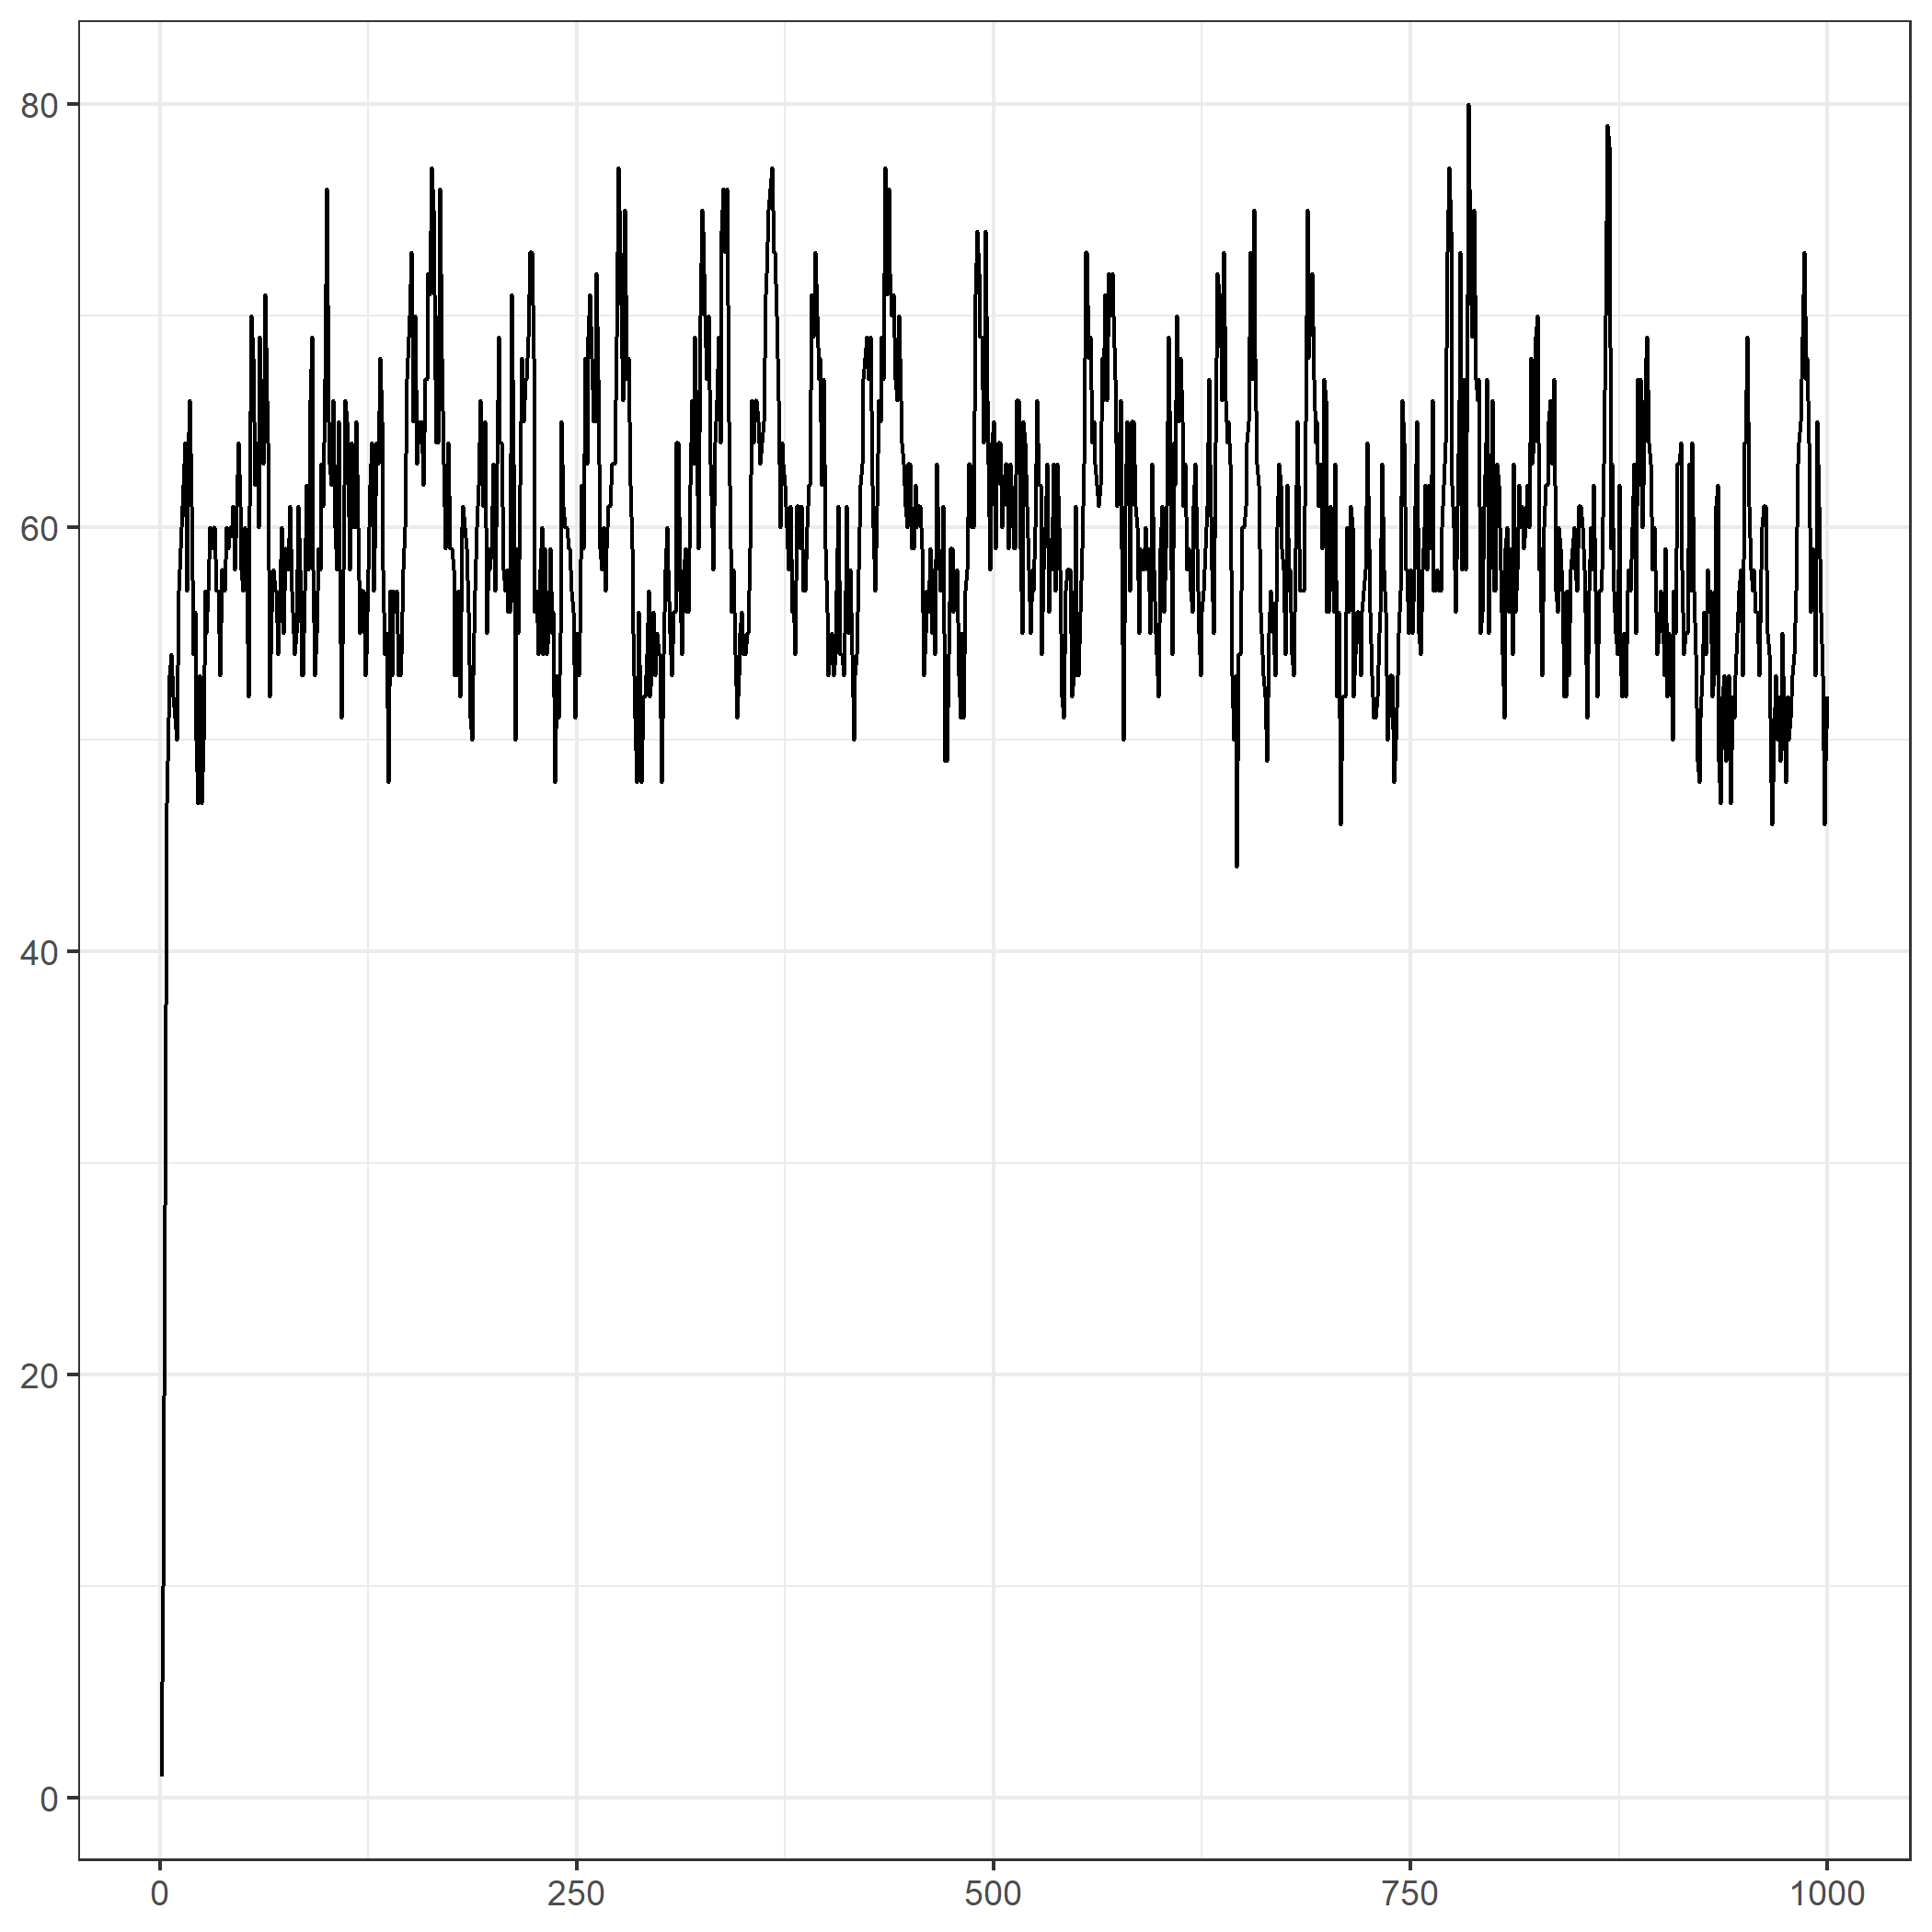
\includegraphics[width=0.6\textwidth]{../notes/figures/sim_overlap_trace} 
		\caption{Representative traceplot of overlap between files from simulation study in Section \ref{accuracy}}\label{fig:sim_overlap_trace}
	\end{center}
\end{figure}



\begin{figure}[!h]
	\begin{center}
		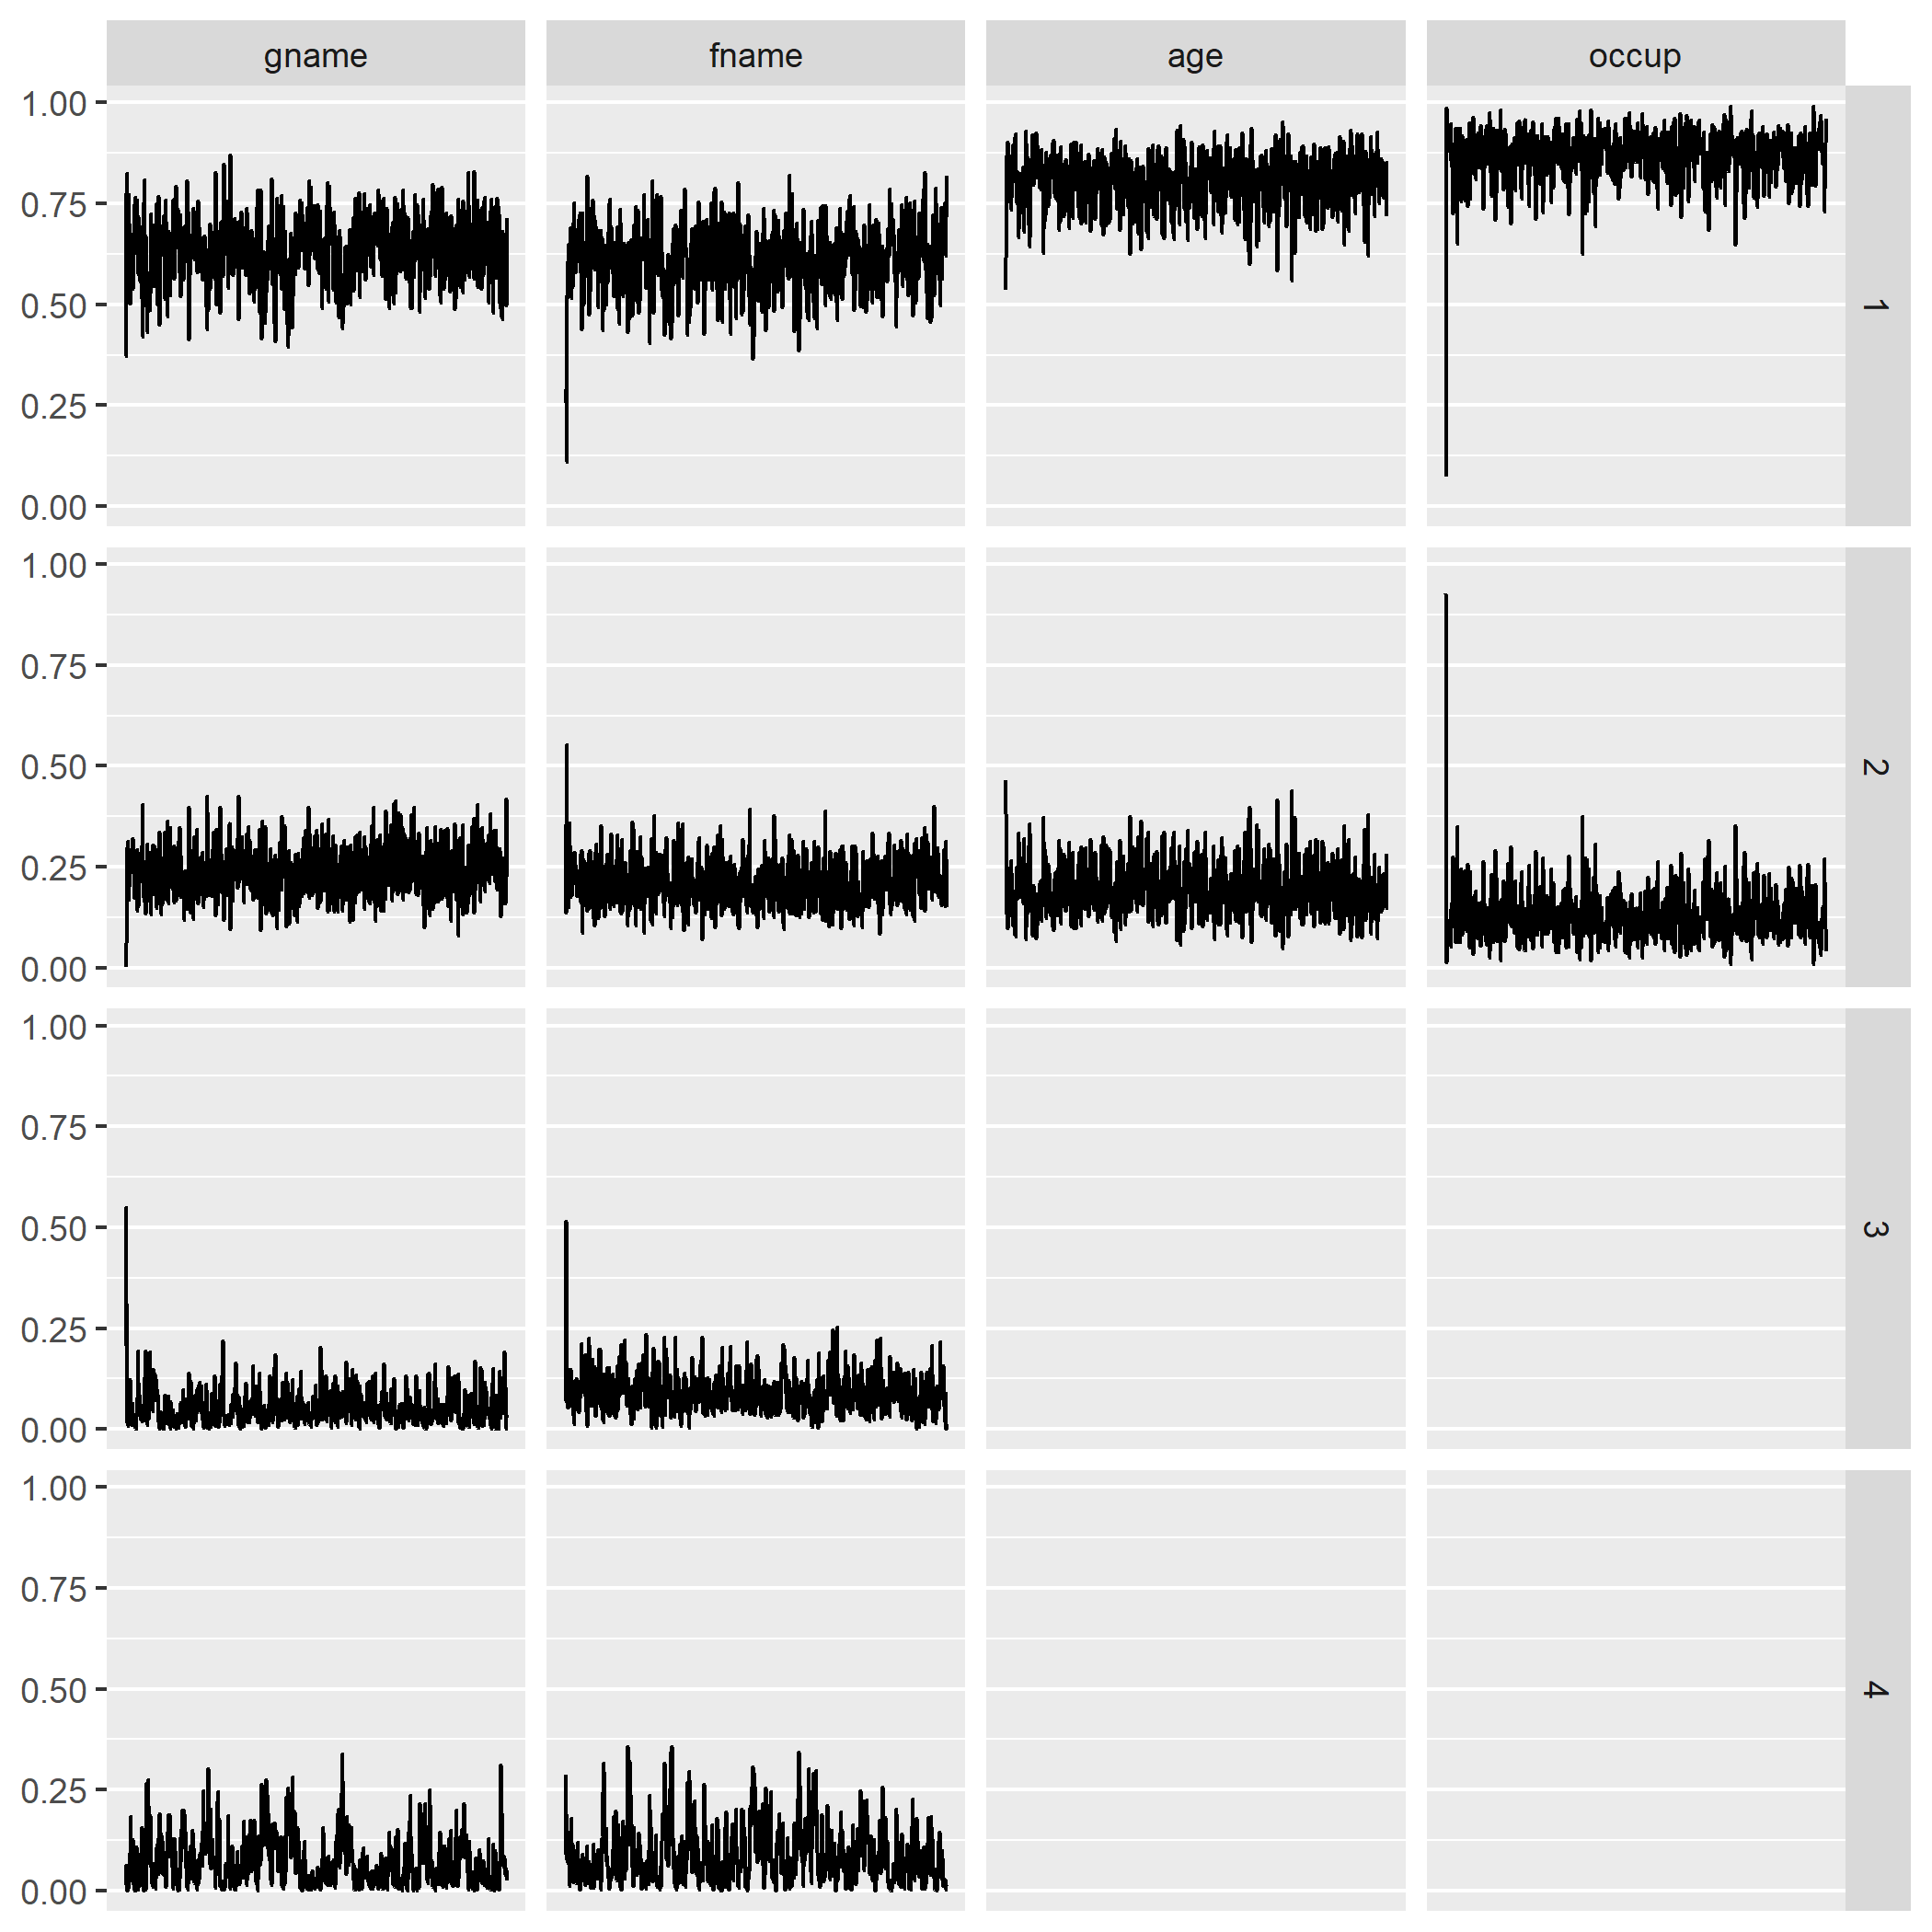
\includegraphics[width=0.6\textwidth]{../notes/figures/sim_m_trace} 
		\caption{Representative traceplot of m parameter from simulation study in Section \ref{accuracy}}\label{fig:sim_m_trace}
	\end{center}
\end{figure}

\begin{figure}[!h]
	\begin{center}
		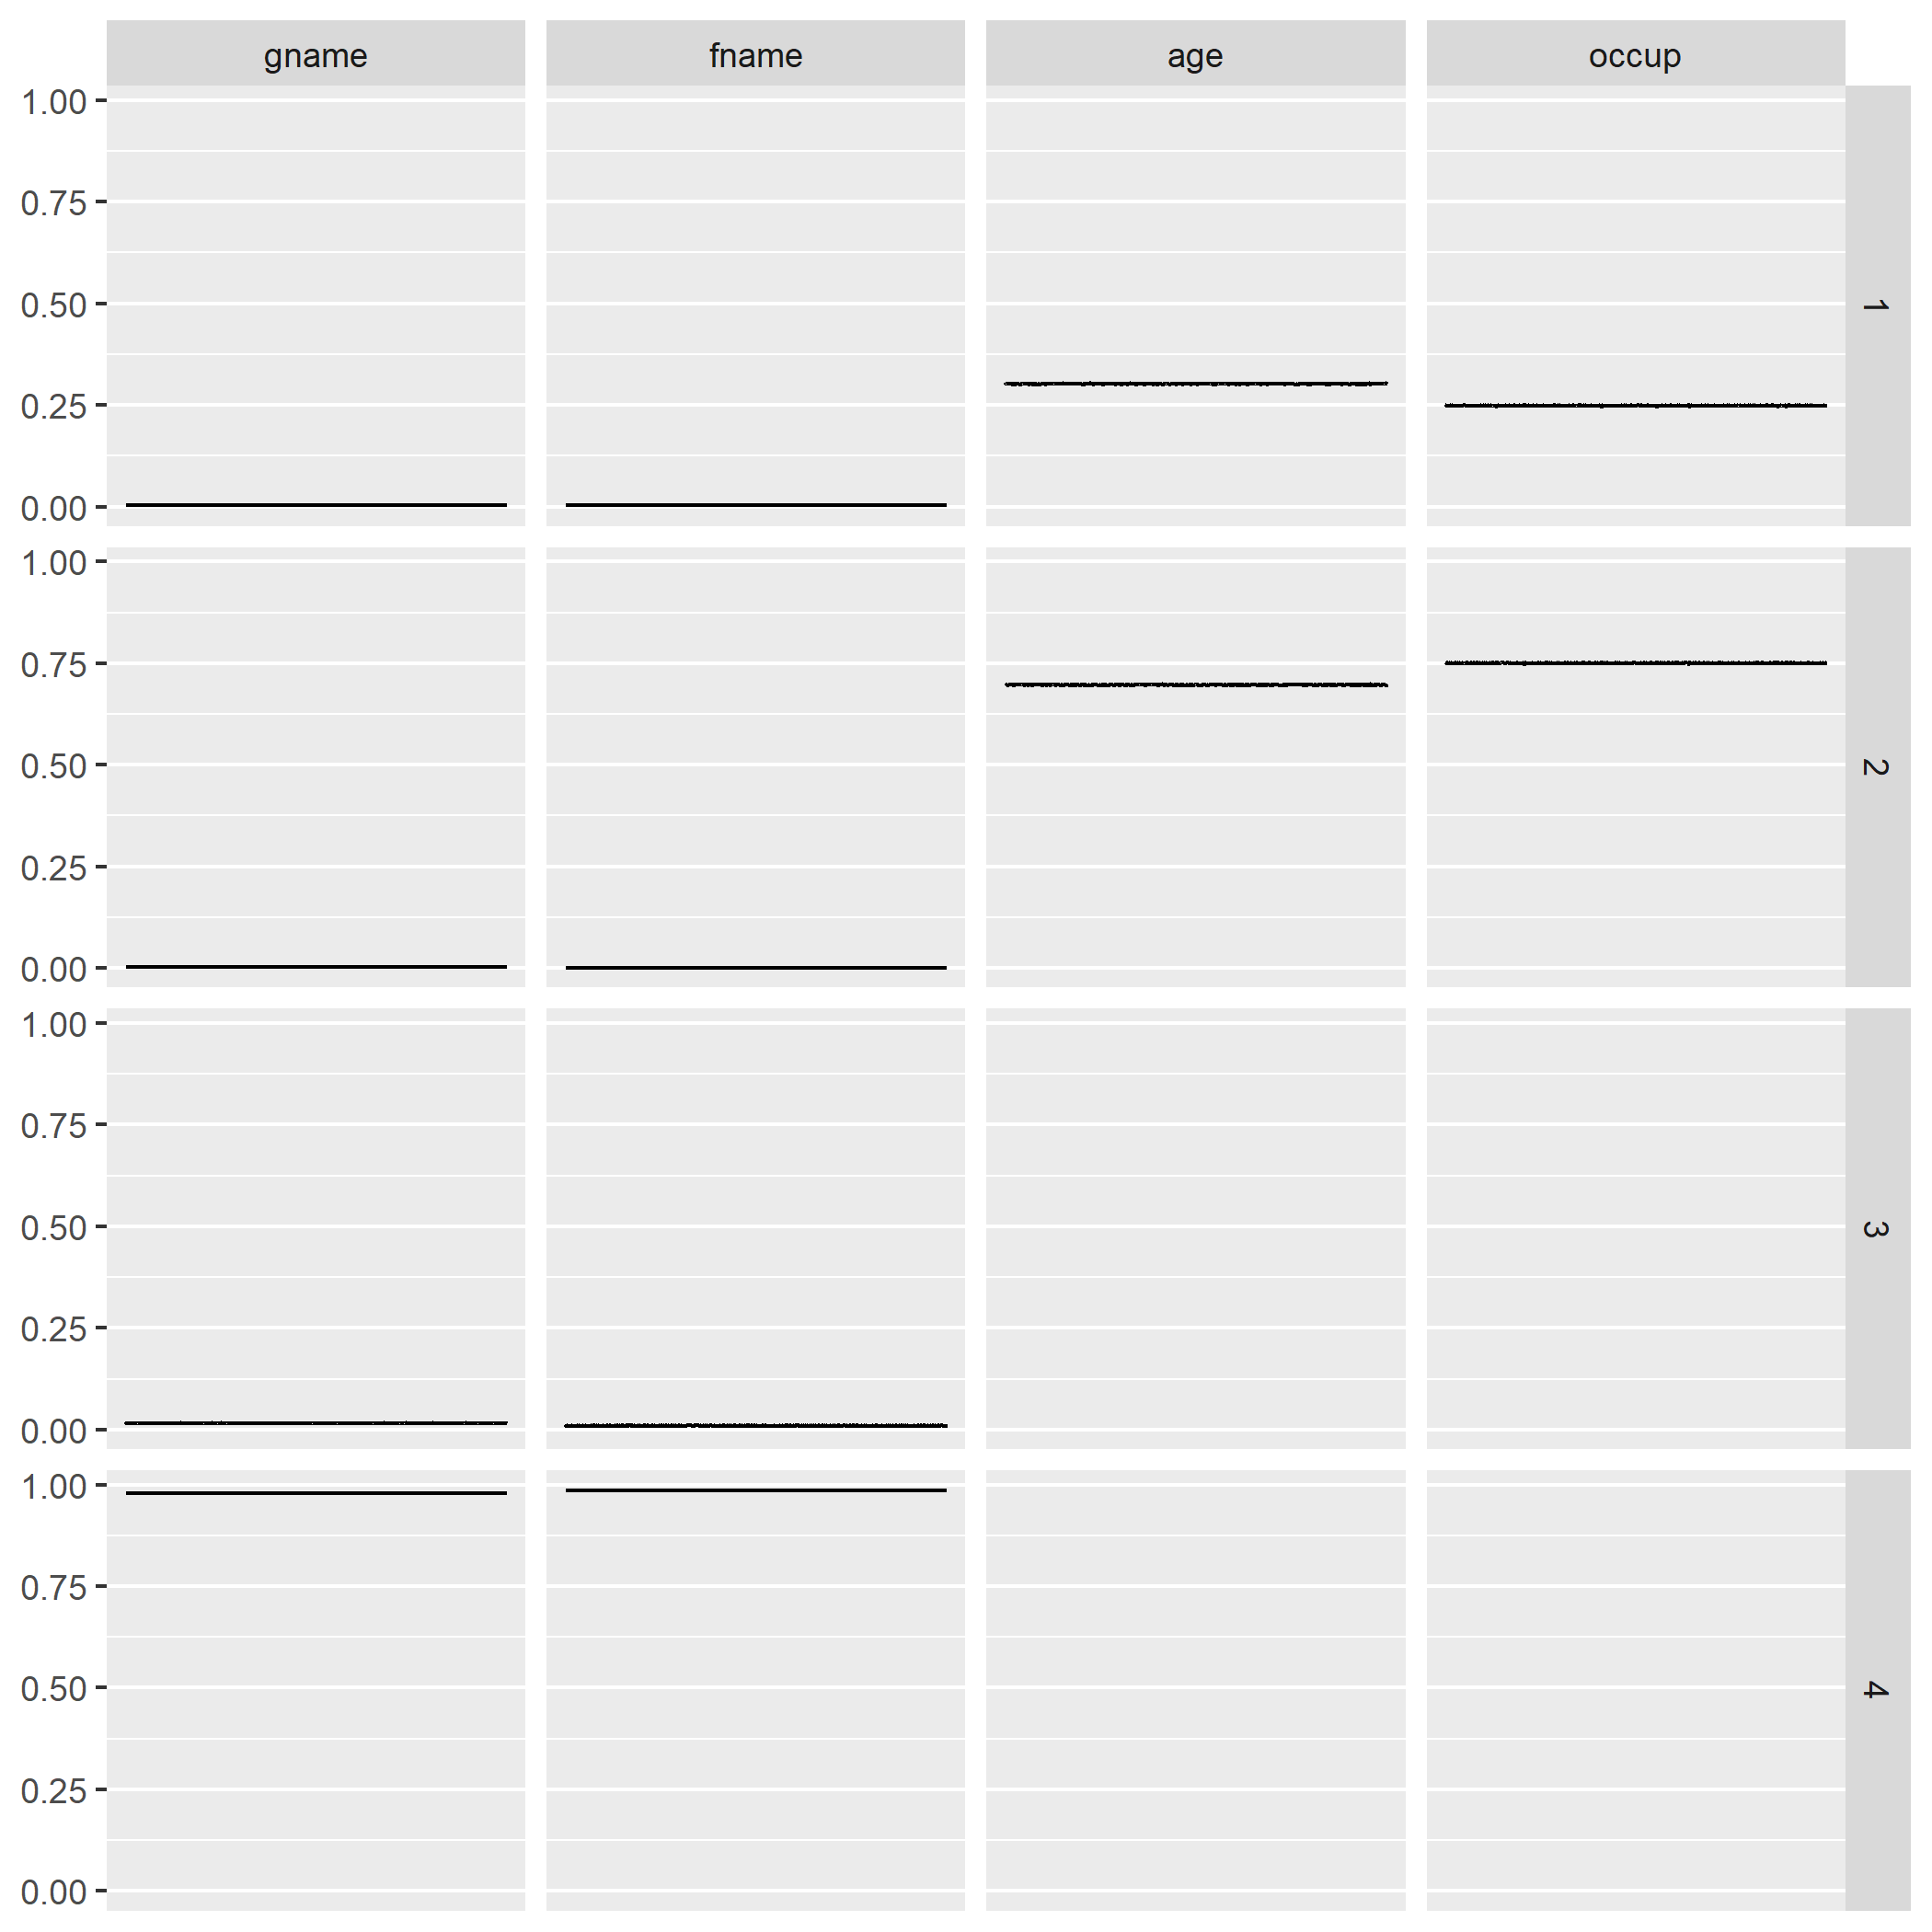
\includegraphics[width=0.6\textwidth]{../notes/figures/sim_u_trace} 
		\caption{Representative traceplot of u parameters from simulation study in Section \ref{accuracy}}\label{fig:sim_u_trace}
	\end{center}
\end{figure}

\clearpage

\hypertarget{appendix-es}{%
	\subsection{Traceplots for El Salvador Case Study}\label{app:appendix-es}}

\begin{figure}[!h]
\begin{center}
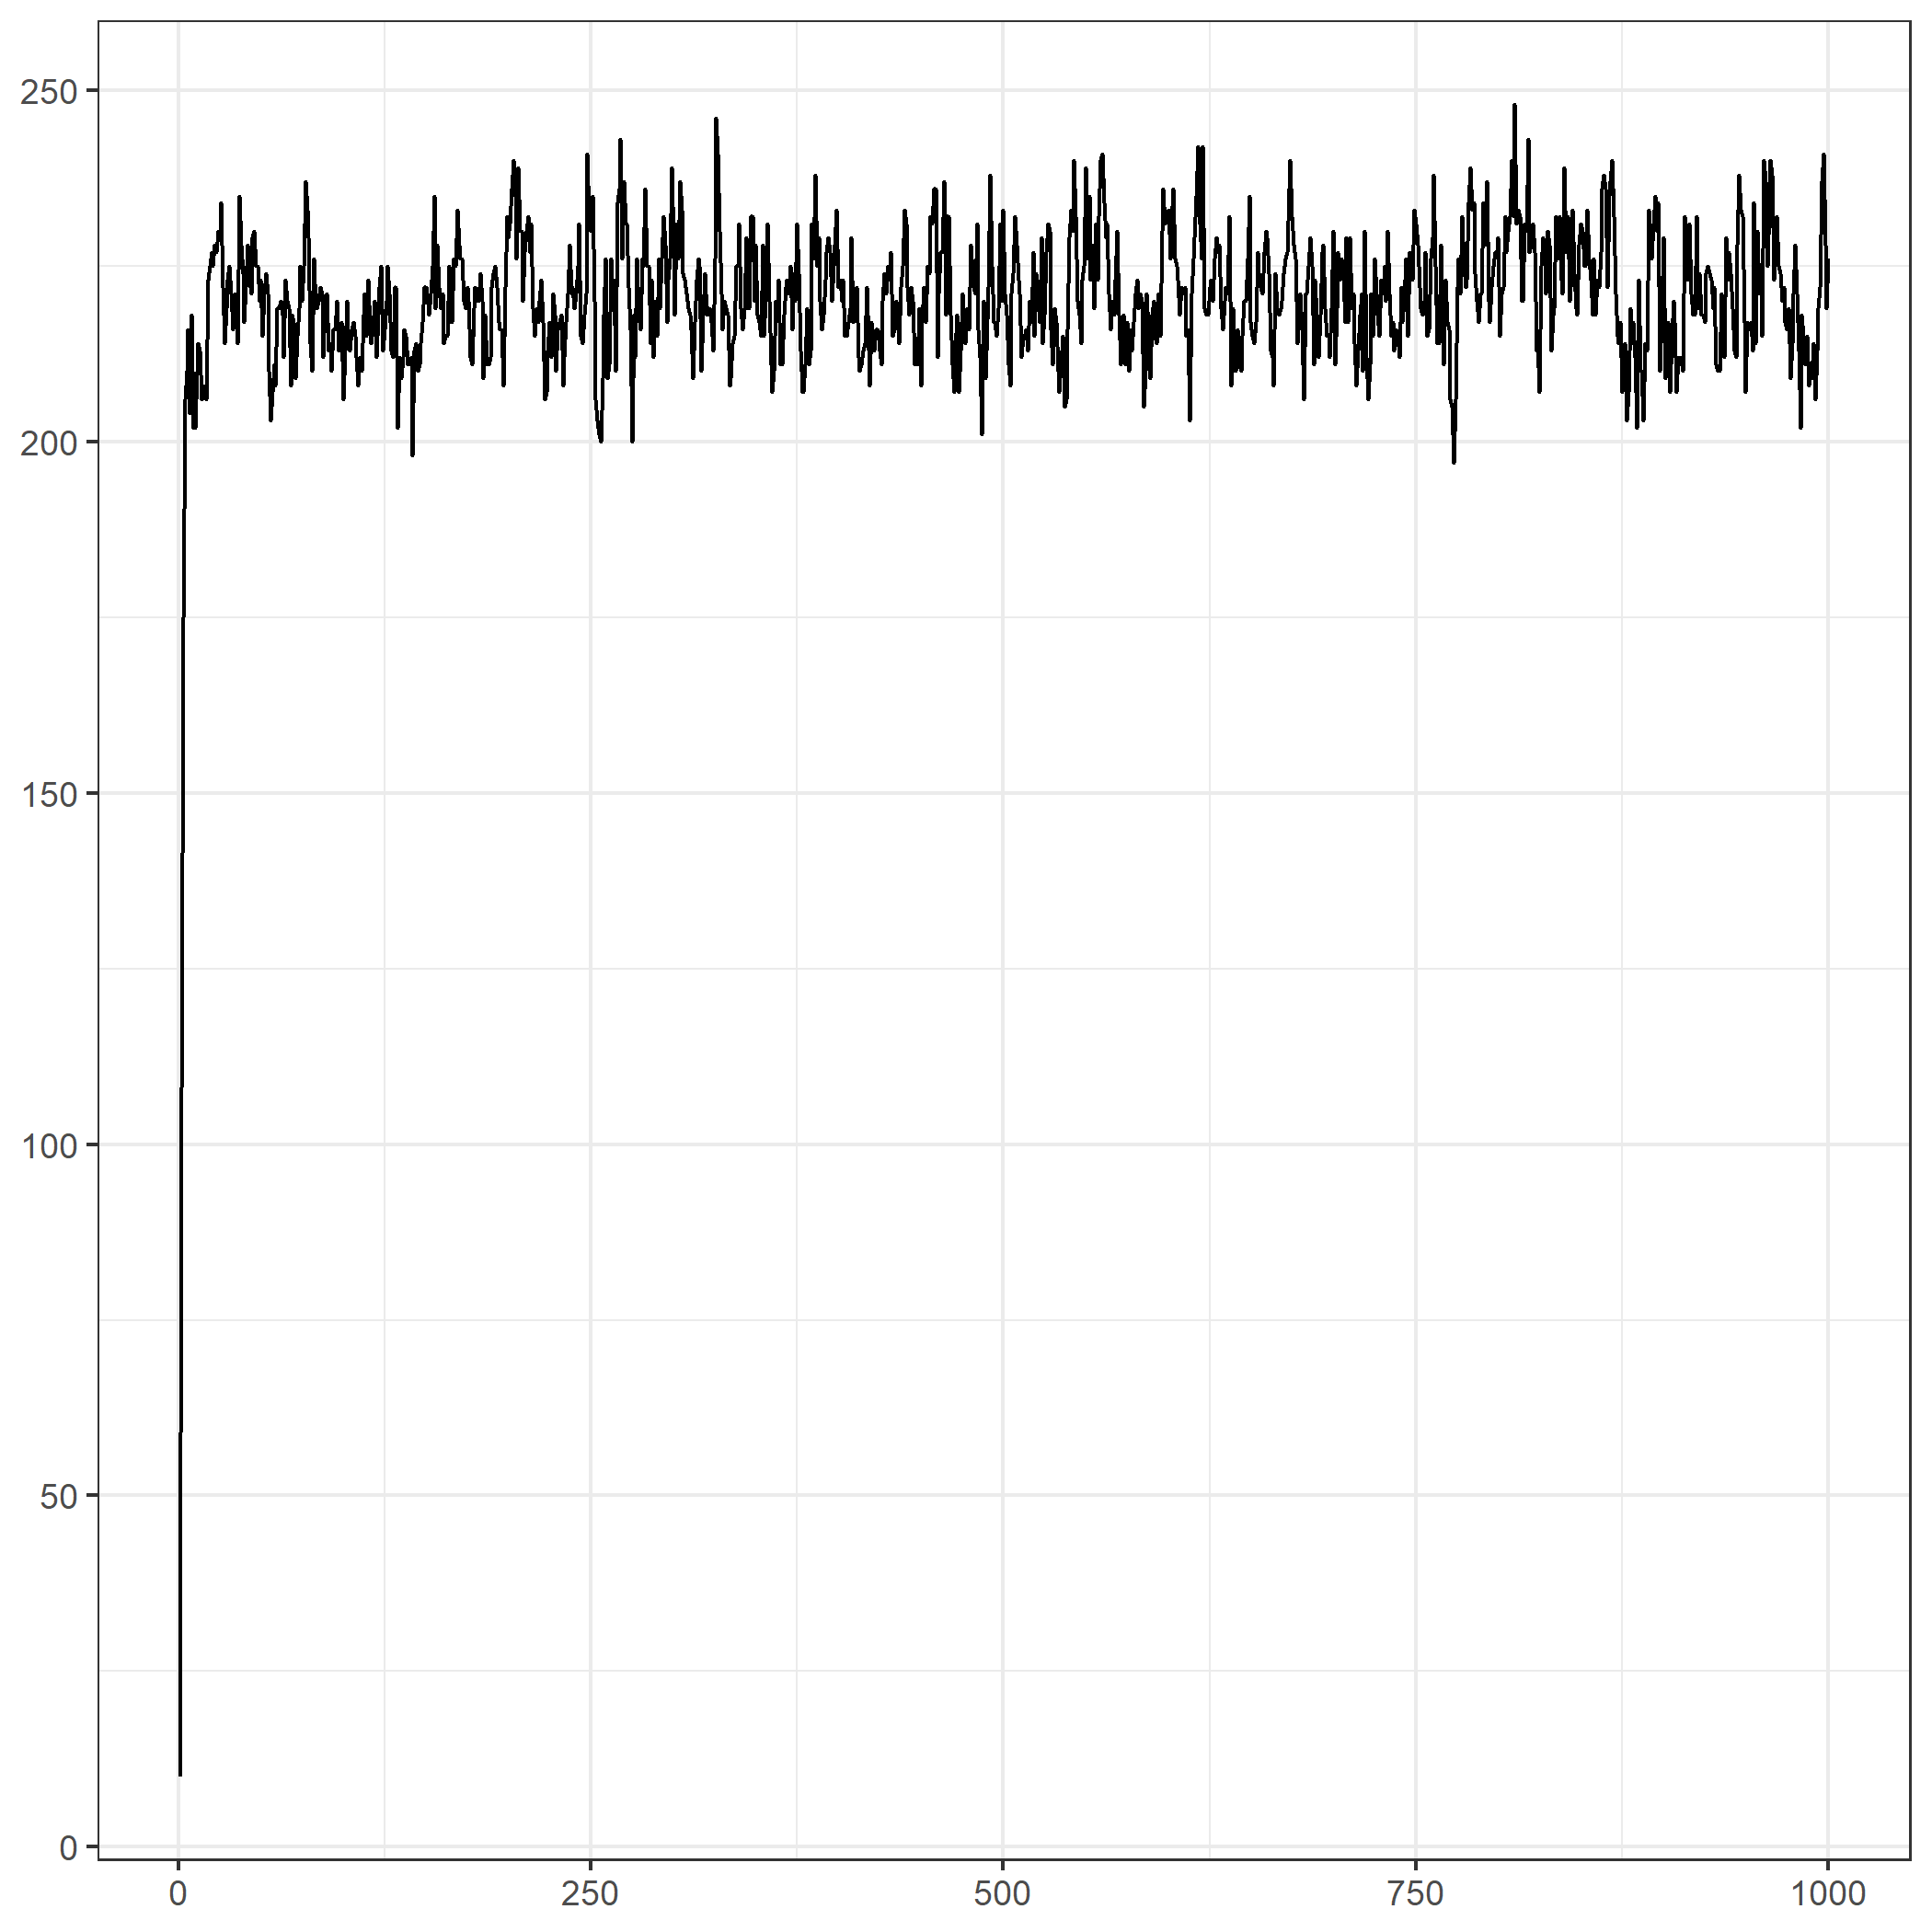
\includegraphics[width=0.6\textwidth]{../notes/figures/el_salvador/overlap_trace} 
\caption{Traceplot for number of matches found across datasets in El Salvador case study}\label{fig:overlap_trace}
\end{center}
\end{figure}

\begin{figure}[!h]
\begin{center}
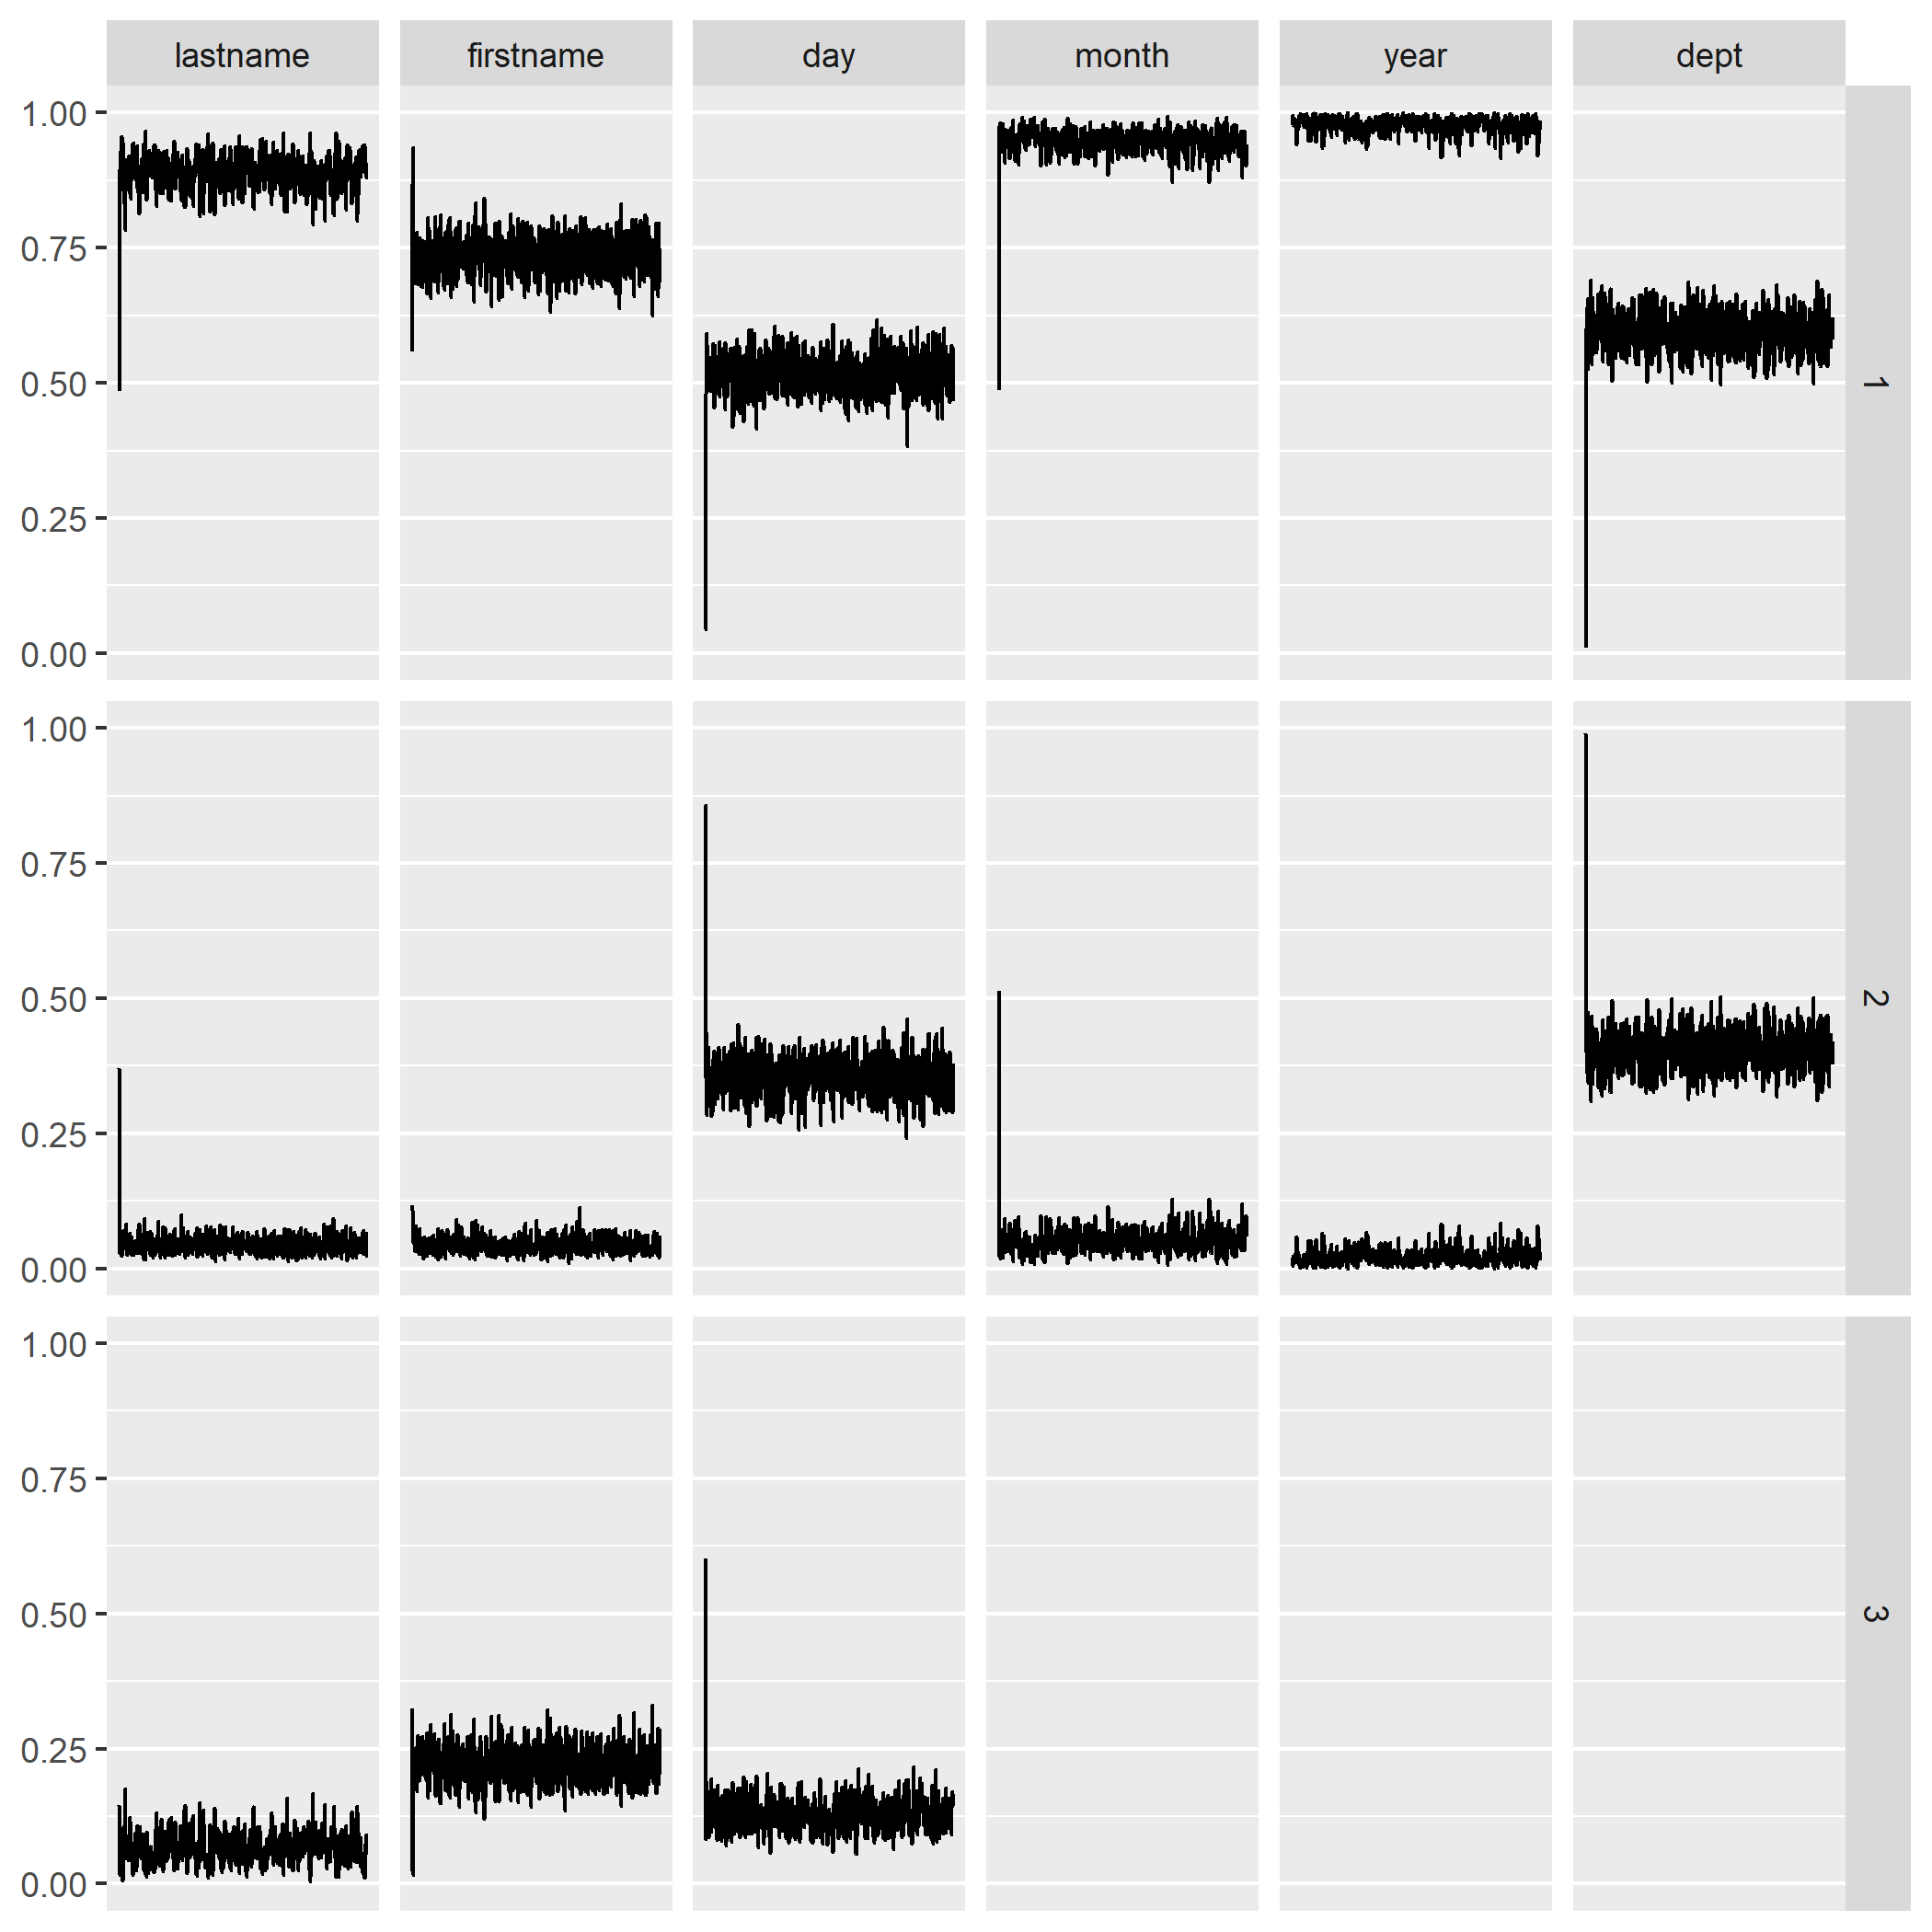
\includegraphics[width=0.6\textwidth]{../notes/figures/el_salvador/m_trace} 
\caption{Traceplot for m parameter in El Salvador case study}\label{fig:m_trace}
\end{center}
\end{figure}

\begin{figure}[!h]
\begin{center}
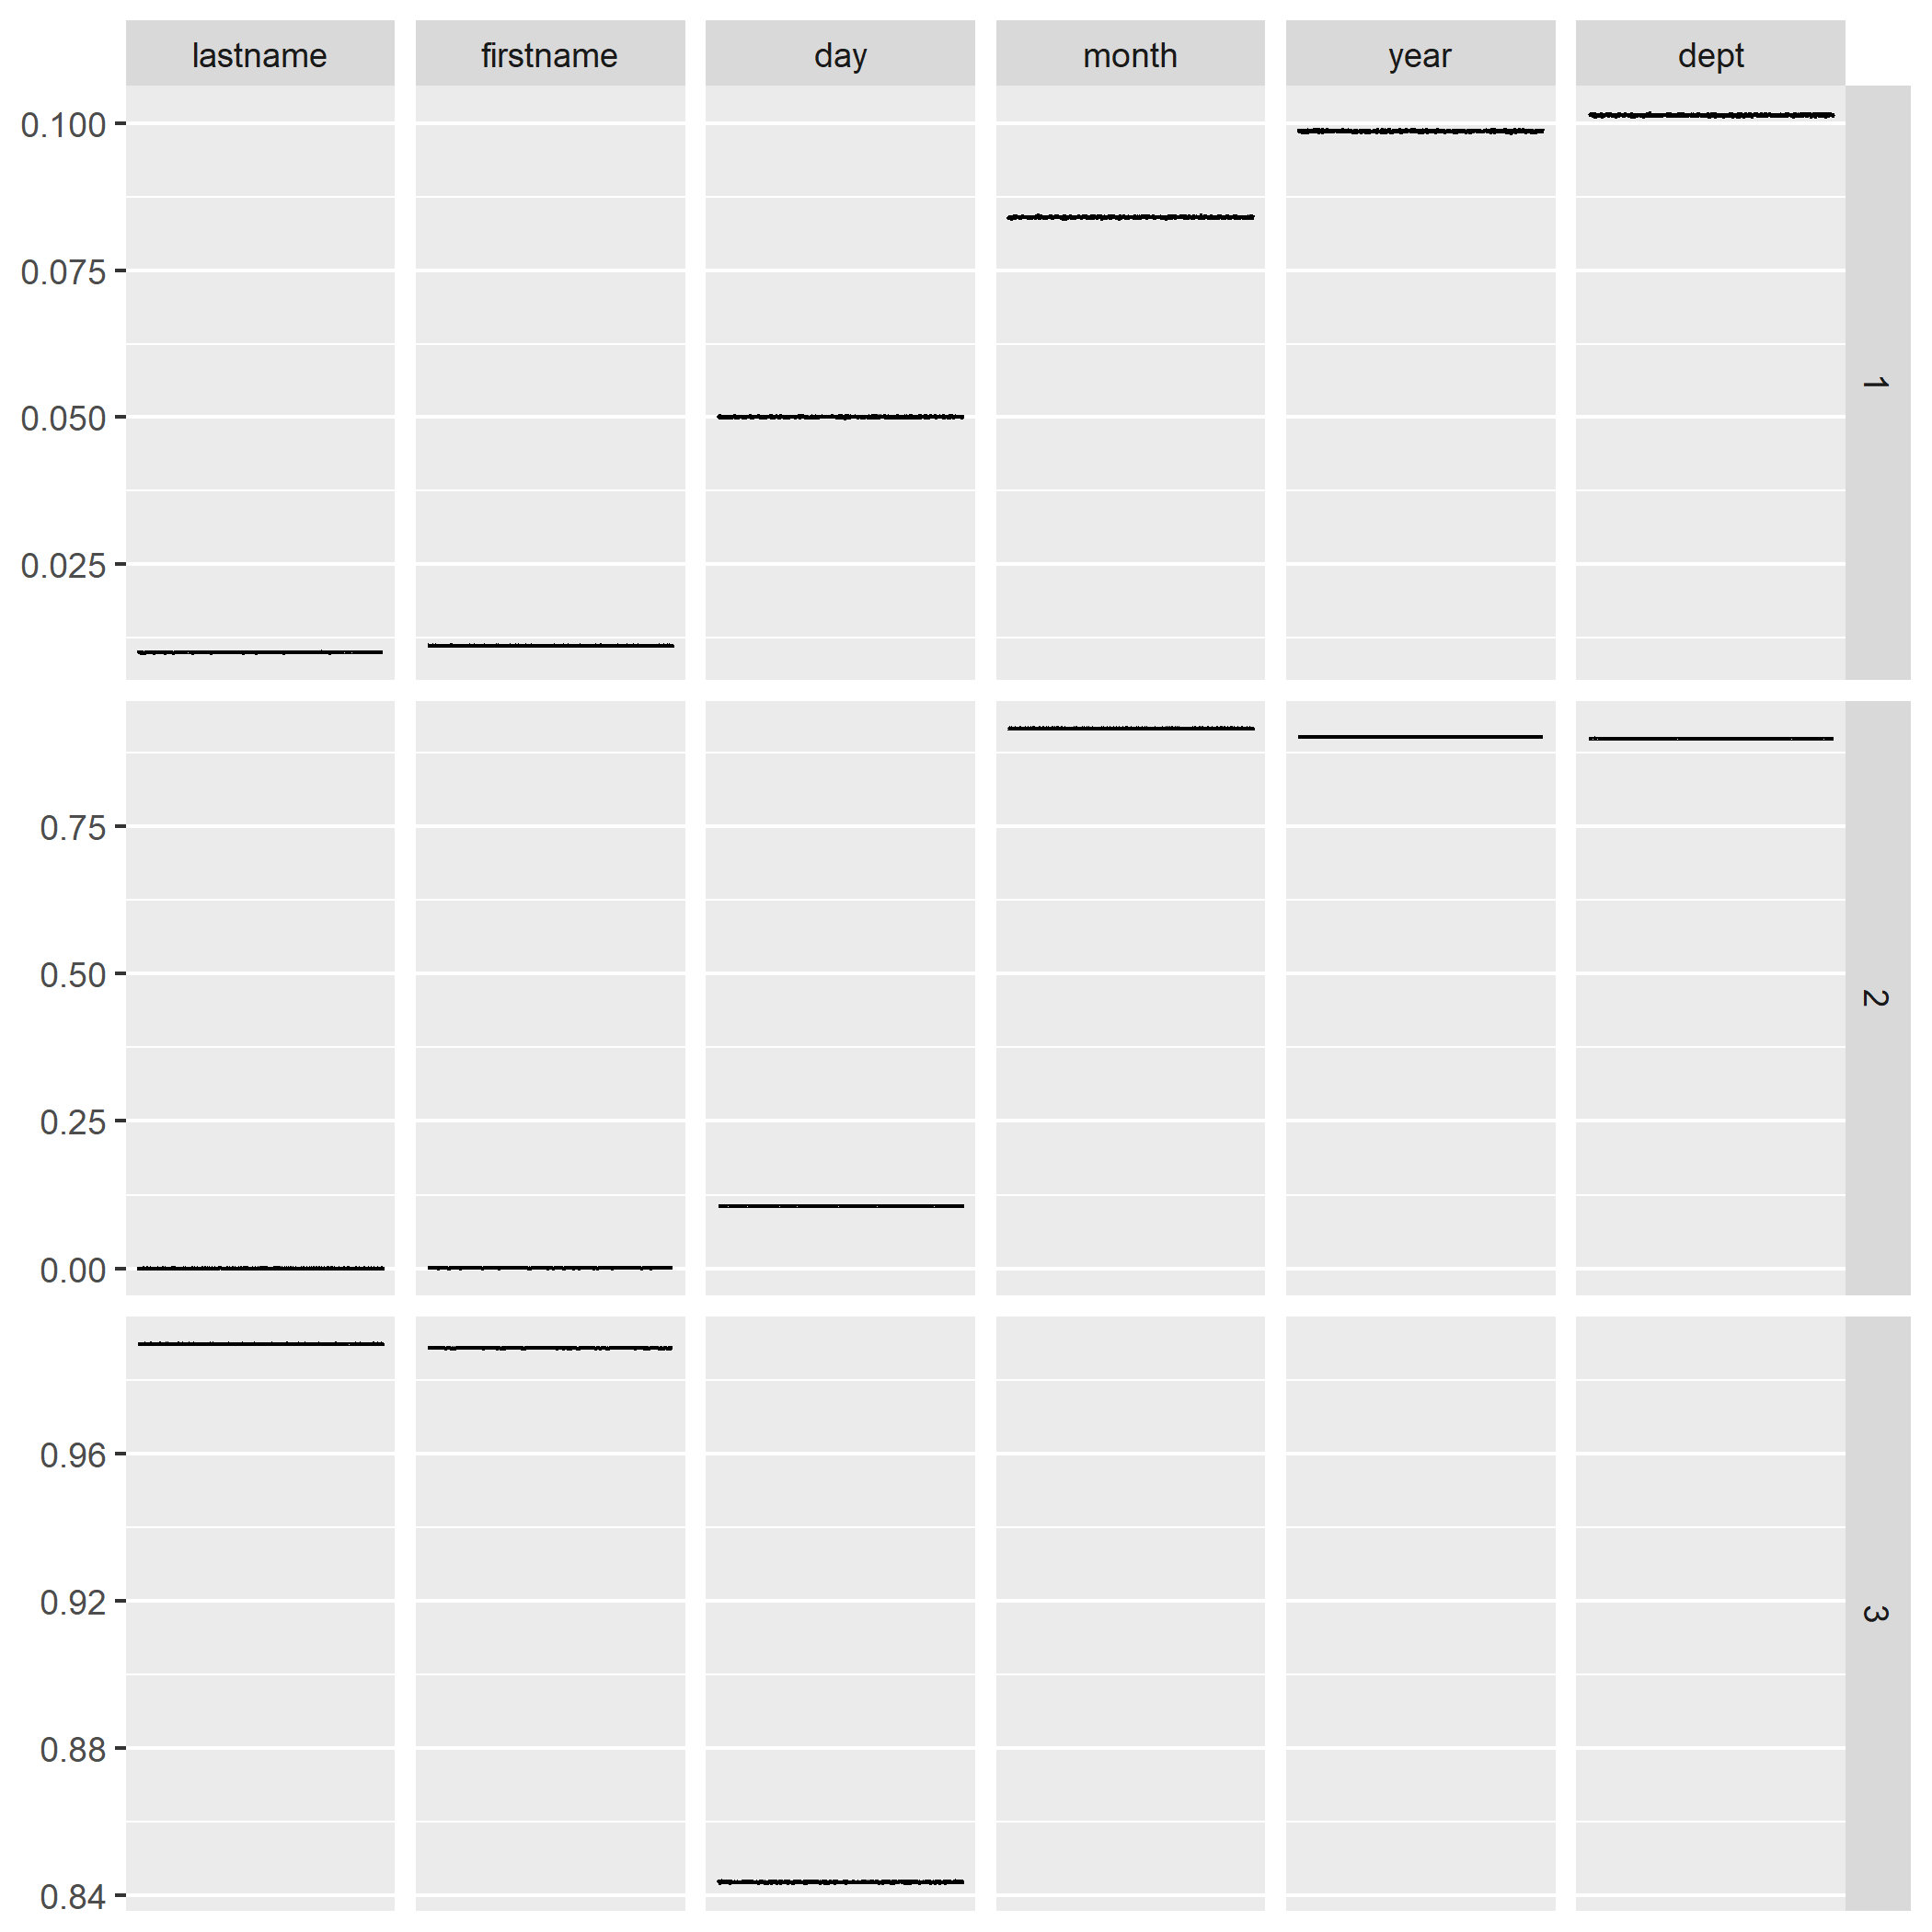
\includegraphics[width=0.6\textwidth]{../notes/figures/el_salvador/u_trace} 
\caption{Traceplot for u parameter in El Salvador case study}\label{fig:u_trace}
\end{center}
\end{figure}




\end{document}
